% Organizing document for the Infernal User's Guide
%
% SVN $Id$


\documentclass[10pt]{article}
%\usepackage{helvetic}
\usepackage{times}
\usepackage{fullpage}
\usepackage{fancybox}  % Must include fancybox *before* fancyvrb;
\usepackage{fancyvrb}  % don't know why.
\usepackage[pdftex]{graphicx}
\usepackage{url}
%\usepackage[backref,colorlinks]{hyperref}
\usepackage[authoryear]{natbib}

\usepackage{verbatim}

\setcounter{secnumdepth}{1}
\renewcommand{\familydefault}{\sfdefault}
% customizations used in the User's Guide


% Description-like environment for documenting functions/APIs.
% puts the description label in a minipage with a large hanging
% indent.
% Good christ this took a long time to develop.
% hanging indent trick stolen from Peter Wilson's hanging.sty @CTAN
% minipage allows multi-line label, and puts item on next line.
% customized list inspired by Kopka/Daly _Guide to LaTeX_ p.213
% SRE, Wed Dec 27 11:37:18 2000
%
\newenvironment{sreapi}{%
     \begin{list}{}{%
       \renewcommand{\makelabel}[1]{%
         \begin{minipage}{\textwidth}%
           \hangindent10em\hangafter1\noindent%
           {\bfseries\texttt{##1}\vspace{0.8em}}%
         \end{minipage}%
     }}}%
     {\end{list}}


% Description-like environment for producing lists like:
%
%     label  stuff, stuff, stuff
%
%    label2  more stuff, more stuff,
%            more stuff.
% \begin{sreitems}{Longest label} \item[label] stuff, ... \end{sreitems}
% SRE, Wed Dec 27 11:59:43 2000
%
\newenvironment{sreitems}[1]{%
     \begin{list}{}{%
       \settowidth{\labelwidth}{#1}%
       \setlength{\leftmargin}{\labelwidth}%
       \addtolength{\leftmargin}{\labelsep}%
       }}
     {\end{list}}
       
\DefineVerbatimEnvironment{sreoutput}{Verbatim}{fontsize=\scriptsize,xleftmargin=2.0\parindent}%
\DefineVerbatimEnvironment{tinysreoutput}{Verbatim}{fontsize=\tiny,xleftmargin=2.0\parindent}%

\makeatletter
\newcommand{\listoffaqs}{\@starttoc{faq}}
\newenvironment{srefaq}[1]
{\addcontentsline{faq}{faq}{#1}\begin{sloppypar}\noindent\slshape\small\begin{quote}\textbf{$\triangleright$ #1}}
{\end{quote}\end{sloppypar}}
\newcommand{\l@faq}[2]{\@dottedtocline{0}{0pt}{0pt}{#1}{#2}}
\makeatother

% Consistent font styles
%   \software{} for the name of a software package
%   \database{} for the name of a database
%   \prog{}     for a program or file name
%   \emprog{}   for an emphasized program or file name
%   \user{}     for a typed user command
%   \response{} for an output line following a \user command
%   \ccode{}    for an inlined C code phrase
\newcommand{\software}[1]{\textsc{#1}}
\newcommand{\database}[1]{\textsc{#1}}
\newcommand{\prog}[1]{{\small\texttt{#1}}}
\newcommand{\emprog}[1]{{\small\bfseries\texttt{#1}}}
\newcommand{\user}[1]{\indent\indent{\small\bfseries\texttt{> #1}}}
\newcommand{\response}[1]{\indent\indent{\small\bfseries\texttt{#1}}}
\newcommand{\ccode}[1]{{\small\texttt{#1}}}

\DefineVerbatimEnvironment{cchunk}{Verbatim}{fontsize=\scriptsize,xleftmargin=2.0\parindent}%

% The ``wideitem'' environment is mostly obsolete, but
% it gets used in converted manpages.
% 
\newenvironment{wideitem}{\begin{list} 
     {}
     { \setlength{\labelwidth}{2in}\setlength{\leftmargin}{1.5in}}}
     {\end{list}}

% The following are used as temp vars in how man pages are 
% converted into LaTeX w/ rman; see ``make manpages'' in Makefile.
%
\newlength{\sresavei}
\newlength{\sresaves}

\def\argmax{\mathop{\mathrm{argmax}}\limits}
\def\argmin{\mathop{\mathrm{argmin}}\limits}

% The sidebar environment, for inserting ``asides''.
% Requires the ``fancybox'' package.
% Example:
%   \usepackage{fancybox}
%   ...
%   \begin{sidebar}
%   \sidebarhead{An aside on string theory.}
%   String theory is not mentioned in this document.
%   \end{sidebar}
%
% SRE, Sun Nov  6 14:45:32 2005
%
\newenvironment{sidebar}%
  {\begin{Sbox}\begin{minipage}{\textwidth}\setlength{\parskip}{0.5em}}%
  {\end{minipage}\end{Sbox}%
   \begin{figure}[htp]\shadowbox{\TheSbox}\end{figure}%
   \setlength{\parskip}{0em}}
\newcommand{\sidebarhead}[1]{{\bfseries{#1}}\vspace{0.3em}}


\begin{document}

\bibliographystyle{apalike}

\begin{titlepage}
{\Large

\vspace*{\fill}

\noindent
{\Huge{Easel}} \\ 
\rule[2pt]{\textwidth}{1pt} \\
\hspace*{\fill} {\large {A library of C functions for
    biological sequence analysis} \\ }

\vspace*{\fill}

\begin{center}
\url{http://bioeasel.org/}\\
Version 0.3dev; February 2016 \\ 

\vspace*{\fill}

Sean R. Eddy\\
HHMI/Harvard University\\
Dept. of Molecular and Cellular Biology\\
Biological Laboratories 1008B\\
16 Divinity Avenue\\
Cambridge, Massachusetts 02138\\
\url{http://eddylab.org/}\\
\end{center}

\vspace*{\fill}
}
\end{titlepage}

\vspace*{\fill}
\begin{flushleft}
Copyright (C) 2016 Howard Hughes Medical Institute.

\vspace{2em} 

Easel is open source.  Easel's source code and documentation are
freely redistributable and modifiable under the terms of the Berkeley
Software Distribution License (BSD 2 Clause;
\url{https://opensource.org/licenses/BSD-2-Clause}).

\end{flushleft}









\newpage
\tableofcontents

\newpage
\section{Introduction}
\setcounter{footnote}{0}

HMMER is used to search sequence databases for homologs of protein
or DNA sequences, and to make sequence alignments. HMMER can be used
to search sequence databases with single query sequences but it
becomes particularly powerful when the query is an alignment of multiple
instances of a sequence family. HMMER makes a \emph{profile}
of the query that assigns a position-specific scoring system for
substitutions, insertions, and deletions. HMMER profiles are
probabilistic models called ``profile hidden Markov models'' (profile
HMMs) \citep{Krogh94,Eddy98,Durbin98}.

Compared to BLAST, FASTA, and other sequence alignment and database
search tools based on older scoring methodology, HMMER aims to be
significantly more accurate and more able to detect remote homologs,
because of the strength of its underlying probability models. In the
past, this strength came at a significant computational cost, with
profile HMM implementations running about 100x slower than comparable
BLAST searches for protein search, and about 1000x slower than BLAST
searches for DNA search. With HMMER3.1, HMMER is now essentially as 
fast as BLAST for protein search, and roughly 5-10x slower than BLAST 
in DNA search\footnote{NCBI blastn with \texttt{--wordsize 7}; 
default wordsize of 11 is $\sim$10x faster, but much less sensitive.}.

\subsection{How to avoid reading this manual}

We hate reading documentation. If you're like us, you're sitting here
thinking, \pageref{manualend} pages of documentation, you must be
joking! I just want to know that the software compiles, runs, and
gives apparently useful results, before I read some 
\pageref{manualend} exhausting pages of someone's documentation. For
cynics that have seen one too many software packages that don't
work:

\begin{itemize}
\item Follow the quick installation instructions on page
      \pageref{section:installation}. An automated test suite
      is included, so you will know immediately if something
      went wrong.\footnote{Nothing should go wrong.}
\item Go to the tutorial section on page
\pageref{section:tutorial}, which walks you through some examples of
using HMMER on real data.
\end{itemize}

Everything else, you can come back and read later.



\subsection{How to avoid using this software (links to similar software)}

Several implementations of profile HMM methods and related
position-specific scoring matrix methods are available. 

\begin{center}
\begin{tabular}{lp{5in}l}
Software  &   URL \\ \hline
HMMER     & \url{http://hmmer.org/}\\
SAM       & \url{http://www.cse.ucsc.edu/research/compbio/sam.html}\\
PSI-BLAST & \url{http://www.ncbi.nlm.nih.gov/Education/BLASTinfo/psi1.htm}\\
PFTOOLS   & \url{http://www.isrec.isb-sib.ch/profile/profile.html}\\
\end{tabular}
\end{center}

The UC Santa Cruz SAM software is the closest relative of HMMER.


\subsection{What profile HMMs are}

Profile HMMs are statistical models of multiple sequence alignments,
or even of single sequences. They capture position-specific information about
how conserved each column of the alignment is, and which 
residues\footnote{In some circles, ``residue" is used to refer specifically in
reference to amino acids, but here we allow the term to alternately refer
to nucleotides.} are likely. Anders Krogh, David Haussler, and co-workers at UC
Santa Cruz introduced profile HMMs to computational biology \citep{Krogh94}, 
adopting HMM techniques which have been used for years in speech recognition.
HMMs had been used in biology before the Krogh/Haussler work, notably by Gary
Churchill \citep{Churchill89}, but the Krogh paper had a dramatic impact
because HMM technology was so well-suited to the popular ``profile'' methods
for searching databases using multiple sequence alignments instead of single
query sequences.

``Profiles'' had been introduced by Gribskov and colleagues
\citep{Gribskov87,Gribskov90}, and several other groups introduced
similar approaches at about the same time, such as ``flexible
patterns'' \citep{Barton90}, and
``templates''\citep{Bashford87,Taylor86}. The term ``profile'' has
stuck.\footnote{There has been agitation in some quarters to call all
  such models ``position specific scoring matrices'', PSSMs, but
  certain small nocturnal North American marsupials have a prior claim
  on the name.}  All profile methods (including PSI-BLAST
\citep{Altschul97}) are more or less statistical descriptions of the
consensus of a multiple sequence alignment. They use
\emph{position-specific} scores for amino acids or nucleotides (residues)
and position specific penalties for opening and extending an insertion or
deletion.  Traditional pairwise alignment (for example, BLAST
\citep{Altschul90}, FASTA \citep{Pearson88}, or the Smith/Waterman
algorithm \citep{Smith81}) uses position-{\em independent} scoring
parameters. This property of profiles captures important information
about the degree of conservation at various positions in the multiple
alignment, and the varying degree to which gaps and insertions are
permitted.

The advantage of using HMMs is that HMMs have a formal probabilistic
basis. We use probability theory to guide how all the scoring
parameters should be set. Though this might sound like a purely
academic issue, this probabilistic basis lets us do things that more
heuristic methods cannot do easily. One of the most important is that
HMMs have a consistent theory for setting position-specific gap and
insertion scores. The methods are consistent and therefore highly
automatable, allowing us to make libraries of hundreds of profile HMMs
and apply them on a very large scale to whole genome analysis.  One
such database of protein domain models is Pfam
\citep{Sonnhammer97,Finn10}, which is a significant part of the
Interpro protein domain annotation system \citep{Mulder03}. The
construction and use of Pfam is tightly tied to the HMMER software
package.

Profile HMMs do have important limitations. One is that HMMs do not
capture any higher-order correlations.  An HMM assumes that the
identity of a particular position is independent of the identity of
all other positions.\footnote{This is not strictly true. There is a
  subtle difference between an HMM's state path (a first order Markov
  chain) and the sequence described by an HMM (generated from the
  state path by independent emissions of symbols at each state).}
Profile HMMs are often not good models of structural RNAs, for
instance, because an HMM cannot describe base pairs.



\subsection{Applications of profile HMMs}

HMMER can be used to replace BLASTP and PSI-BLAST for searching protein
databases with single query sequences. HMMER includes two
programs for searching protein databases with single query sequences:
\prog{phmmer} and \prog{jackhmmer}, where \prog{jackhmmer} is an
iterative search akin to PSI-BLAST.

Another application of HMMER is when you are working on a 
sequence family, and you have carefully constructed a multiple
sequence alignment. Your family, like most protein (or DNA) families, has 
a number of strongly (but not absolutely) conserved key amino acids
(or nucleotides), separated by characteristic spacing. You wonder if there 
are more members of your family in the sequence databases, but the family is 
so evolutionarily diverse, a BLAST search with any individual sequence
doesn't even find the rest of the sequences you already know
about. You're sure there are some distantly related sequences in the
noise. You spend many pleasant evenings scanning weak BLAST alignments
by eye to find ones with the right key residues are in the right
places, but you wish there was a computer program that did this a
little better.

Another application is the automated annotation of the domain
structure of proteins. Large databases of curated alignments and HMMER
models of known domains are available, including Pfam \citep{Finn10}
and SMART \citep{Letunic06} in the Interpro database consortium
\citep{Mulder03}. (Many ``top ten protein domains'' lists, a standard
table in genome analysis papers, rely heavily on HMMER annotation.)
Say you have a new sequence that, according to a BLAST analysis, shows
a slew of hits to receptor tyrosine kinases. Before you decide to call
your sequence an RTK homologue, you suspiciously recall that RTK's
are, like many proteins, composed of multiple functional domains, and
these domains are often found promiscuously in proteins with a wide
variety of functions. Is your sequence really an RTK? Or is it a novel
sequence that just happens to have a protein kinase catalytic domain
or fibronectin type III domain?

Another application is the automated construction and maintenance
of large multiple alignment databases.  It is useful to organize
sequences into evolutionarily related families. But there are
thousands of 
sequence families, some of which comprise tens of
thousands of sequences -- and the primary sequence databases continue
to double every year or two. This is a hopeless task for manual
curation; but on the other hand, manual curation is still necessary
for high-quality, biologically relevant multiple alignments. Databases
like Pfam \citep{Finn10} and Dfam \citep{Wheeler13} are constructed by
distinguishing between a stable curated ``seed'' alignment of a small number
of representative sequences, and ``full'' alignments of all detectable
homologs; HMMER is used to make a model of the seed, search the database for
homologs, and can automatically produce the full alignment by aligning every
sequence to the seed consensus.

You may find other applications as well. Using hidden Markov models to
make a linear consensus model of a bunch of related strings is a
pretty generic problem, and not just in biological sequence analysis.
HMMER3 has been used to model mouse song [Elena Rivas, personal
  communication] and in the past HMMER has reportedly been used to
model music, speech, and even automobile engine
telemetry.\footnote{True. We told the company that did it that we now
  live in fear of our own error messages showing up on our car's
  dashboard.}  If you use it for something particularly strange, we'd
be curious to hear about it.


\subsection{Design goals of HMMER3}

In the past, profile HMM methods were considered to be too
computationally expensive, and BLAST has remained the main workhorse
of sequence similarity searching. The main objective of the HMMER3
project (begun in 2004) is to combine the power of probabilistic
inference with high computational speed. We aim to upgrade some of
molecular biology's most important sequence analysis applications to
use more powerful statistical inference engines, without sacrificing
computational performance.

Specifically, HMMER3 has three main design features:

\begin{description}
\item[\textbf{Explicit representation of alignment uncertainty.}]
  Most sequence alignment analysis tools report only a single
  best-scoring alignment. However, sequence alignments are uncertain,
  and the more distantly related sequences are, the more uncertain
  alignments become. HMMER3 calculates complete posterior alignment
  ensembles rather than single optimal alignments. Posterior ensembles
  get used for a variety of useful inferences involving alignment
  uncertainty. For example, any HMMER sequence alignment is
  accompanied by posterior probability annotation, representing the
  degree of confidence in each individual aligned residue.

\item[\textbf{Sequence scores, not alignment scores.}]  Alignment
  uncertainty has an important impact on the power of sequence
  database searches.  It's precisely the most remote homologs -- the
  most difficult to identify and potentially most interesting
  sequences -- where alignment uncertainty is greatest, and where the
  statistical approximation inherent in scoring just a single best
  alignment breaks down the most. To maximize power to discriminate
  true homologs from nonhomologs in a database search, statistical
  inference theory says you ought to be scoring sequences by
  integrating over alignment uncertainty, not just scoring the single
  best alignment. HMMER3's log-odds scores are sequence scores, not
  just optimal alignment scores; they are integrated over the
  posterior alignment ensemble.
  
\item[\textbf{Speed.}] A major limitation of previous profile HMM
  implementations (including HMMER2) was their slow performance. HMMER3
  implements a heuristic acceleration algorithm. For most protein 
  queries, it's about as fast as BLAST, while for DNA queries it's 
  typically less than 10x slower than sensitive settings for BLAST. 
\end{description}

Individually, none of these points is new. As far as alignment
ensembles and sequence scores go, pretty much the whole reason why
hidden Markov models are so theoretically attractive for sequence
analysis is that they are good probabilistic models for explicitly
dealing with alignment uncertainty. The SAM profile HMM software from
UC Santa Cruz has always used full probabilistic inference (the HMM
Forward and Backward algorithms) as opposed to optimal alignment
scores (the HMM Viterbi algorithm). HMMER2 had the full HMM inference
algorithms available as command-line options, but used Viterbi
alignment by default, in part for speed reasons. Calculating alignment
ensembles is even more computationally intensive than calculating
single optimal alignments.

One reason why it's been hard to deploy sequence scores for practical
large-scale use is that we haven't known how to accurately calculate
the statistical significance of a log-odds score that's been
integrated over alignment uncertainty. Accurate statistical
significance estimates are essential when one is trying to
discriminate homologs from millions of unrelated sequences in a large
sequence database search. The statistical significance of optimal
alignment scores can be calculated by Karlin/Altschul statistics
\citep{Karlin90,KarlinAltschul93}. Karlin/Altschul statistics are one
of the most important and fundamental advances introduced by BLAST.
However, this theory doesn't apply to integrated log-odds sequence
scores (HMM ``Forward scores'').  The statistical significance
(expectation values, or E-values) of HMMER3 sequence scores is
determined by using recent theoretical conjectures about the
statistical properties of integrated log-odds scores which have been
supported by numerical simulation experiments \citep{Eddy08}.

And as far as speed goes, there's really nothing new about HMMER3's
speed either. Besides Karlin/Altschul statistics, the main reason
BLAST has been so useful is that it's so fast.  Our design goal in
HMMER3 was to achieve rough speed parity between BLAST and more formal
and powerful HMM-based methods.  The acceleration algorithm in HMMER3
is a new heuristic. It seems likely to be more sensitive than BLAST's
heuristics on theoretical grounds. It certainly benchmarks that way in
practice, at least in our hands. Additionally, it's very well suited
to modern hardware architectures. We expect to be able to take good
advantage of GPUs and other parallel processing environments in the
near future.

\subsection{What's different in HMMER3, compared to HMMER2}

If you're upgrading from using HMMER2, you will notice these main
issues, among many lesser ones:

\paragraph{Speed.} Did we mention, HMMER3 is 100-1000x faster? No more
coffee breaks waiting for results.

\paragraph{No model calibration: hmmcalibrate is gone.} If you're looking for the
\prog{hmmcalibrate} program, it's not there any more. We understand
the statistics of HMMER scores well enough now that a
compute-intensive calibration step is unnecessary. There's still a
model statistics calibration step but it's tiny by comparison to what
HMMER2 had to do, so now it's built into \prog{hmmbuild}, and into
single sequence searches like \prog{phmmer} and \prog{jackhmmer}.

\paragraph{Local alignments, not glocal alignments.} We only
understand the statistics of HMMER \emph{local} Forward scores, so
HMMER3 (for now) only does local alignment. HMMER2 used glocal
alignment by default (global with respect to the query profile, local
in the target sequence), and had an option for doing local alignment.
Whereas we used to build two HMMER2 models for each Pfam domain (a
glocal mode one and a local mode one) now we build just one HMMER3
model.  Because HMMER3 does local alignment, you'll notice more
ragged-ended annotations of Pfam domains, for example. In a few cases
of short domains, such as zinc fingers, HMMER3 can be less sensitive
than HMMER2, because even though HMMER3's parameterization is more
sensitive than HMMER2's, glocal alignment (when a complete domain is
in fact present) is more sensitive than local. No, we're not happy
about it either, but the benefits greatly outweigh the costs.


\subsection{What's new in HMMER3.1, compared to HMMER 3.0}

\paragraph{DNA sequence comparison.} HMMER now includes tools that are
specifically designed for DNA/DNA comparison: \prog{nhmmer} and
\prog{nhmmscan}. These give the ability to search long
(e.g. chromosome length) target sequences.

\paragraph{More sequence input formats.} HMMER now handles a wide variety of
input sequence file formats, both aligned (Stockholm, Aligned FASTA, Clustal,
NCBI PSI-BLAST, PHYLIP, Selex, UCSC SAM A2M) and unaligned (FASTA, EMBL,
Genbank), usually with autodetection.

\paragraph{MSV stage of HMMER acceleration pipeline now even faster.}
 Bjarne Knudsen, chief scientific officer of CLCbio, contributed an
 important optimization of the MSV filter (the first stage in the
 accelerated "filter pipeline") that increases overall HMMER3 speed by
 about two-fold. 

\paragraph{Faster DNA search using FM-index methods.} This beta release includes a new
option for increasing the speed of searching DNA sequence files. A
binary file is created in a preprocessing step, using the tool
\prog{makehmmerdb}. The tool \prog{nhmmer} then utilizes this binary
format to support a fast new seed-finding stage. Using default
settings in \prog{nhmmer}, we have observed a roughly 10-fold
acceleration with small loss of sensitivity on benchmarks. (This
method has been tested, but should still be treated as somewhat
experimental.)


\subsection{What's still missing in HMMER3.1}

Even though this is a stable public release that we consider suitable
for large-scale production work (genome annotation, Pfam analysis,
whatever), at the same time, HMMER is a work in progress. We think the
codebase is a suitable foundation for development of a number of
significantly improved approaches to classically important problems in
sequence analysis. Some of the more important ``holes'' for us are:

\paragraph{Translated comparisons.} We'd of course love to have the HMM
equivalents of BLASTX, TBLASTN, and TBLASTX. They'll come.

\paragraph{Profile/profile comparison.} A number of pioneering papers and
software packages have demonstrated the power of profile/profile
comparison for even more sensitive remote homology detection. We will
aim to develop profile HMM methods in HMMER with improved detection
power, and at HMMER3 speed.

\vspace{2em}

We also have some technical and usability issues we will be addressing
Real Soon Now:

\paragraph{More alignment modes.} As mentioned above, HMMER3 \emph{only} does local
alignment. HMMER2 also could do glocal alignment (align a complete
model to a subsequence of the target) and global alignment (align a
complete model to a complete target sequence). The E-value statistics
of glocal and global alignment remain poorly understood. HMMER3 relies
on accurate significance statistics, far more so than HMMER2 did,
because HMMER3's acceleration pipeline works by filtering out
sequences with poor P-values.

\paragraph{More speed.} Even on x86 platforms, HMMER3's acceleration
algorithms are still on a nicely sloping bit of their asymptotic
optimization curve. We still think we can accelerate the code by another 
two-fold or so, perhaps more for DNA search. Additionally, for a small number
of HMMs ($<1$\% of Pfam models), the acceleration core is performing relatively
poorly, for reasons we pretty much understand (having to do with biased
composition; most of these pesky models are hydrophobic membrane proteins), but
which are nontrivial to work around. This'll produce an annoying behavior that
you may notice: if you look systematically, sometimes you'll see a model that
runs at something more like HMMER2 speed, 100x or so slower than an average
query. This, needless to say, Will Be Fixed.

\paragraph{More processor support.} One of the attractive features of the
HMMER3 ``MSV'' acceleration algorithm is that it is a very tight and
efficient piece of code, which ought to be able to take advantage of
recent advances in using massively parallel GPUs (graphics processing
units), and other specialized processors such as the Cell processor,
or FPGAs. We have prototype work going on in a variety of processors,
but none of this is far along as yet. But this work (combined with the
parallelization) is partly why we expect to wring significantly more
speed out of HMMER in the future.

\paragraph{Better parallelization.} HMMER3 is so fast that it's often
input-bound, rather than CPU-bound: that is, it takes longer to get at
the sequences than it takes to compare them to a profile. That's
taxing the simple parallelization methods we use. HMMER3's
multithreaded parallelization really doesn't scale well beyond 2-4
processors, on most machines; and possibly worse, if you're on a slow
filesystem (for example, if you're reading data from a network
filesystem instead of from local disk). We need to do a lot more work
on our parallelization and our data input.


\subsection{How to learn more about profile HMMs}

\textbf{Cryptogenomicon} (\url{http://cryptogenomicon.org/}) is a blog
where we will be talking about issues as they arise in HMMER3, and
where you can comment or follow the discussion.

Reviews of the profile HMM literature have been written by us
\citep{Eddy96,Eddy98} and by Anders Krogh \citep{Krogh98}.

For details on how profile HMMs and probabilistic models are used in
computational biology, see the pioneering 1994 paper from Krogh et
al. \citep{Krogh94} or our book \emph{Biological Sequence Analysis:
Probabilistic Models of Proteins and Nucleic Acids} \citep{Durbin98}.

For details on many aspects of the inner workings
of HMMER3, see recent papers by us \citep{Eddy09b,Eddy11}.

To learn more about HMMs from the perspective of the speech
recognition community, an excellent tutorial introduction has been
written by Rabiner \citep{Rabiner89}.

\begin{srefaq}{How do I cite HMMER?}
There is still no ``real'' paper on HMMER. If you're writing for an
enlightened (url-friendly) journal, the best reference is
\url{http://hmmer.org/}.
If you must use a paper reference, the best one to use is our 1998
profile HMM review \citep{Eddy98}.
\end{srefaq}















  











\newpage
\section{Installation}
\label{section:installation}
\setcounter{footnote}{0}

\subsection{Quick installation instructions}

Download \prog{hmmer-3.1b2.tar.gz} from \url{http://hmmer.org/};
%, or
%directly from the ftp
%\url{ftp://selab.janelia.org/pub/software/hmmer3/3.1b2/hmmer-3.1b2.tar.gz};
unpack it:

\user{wget ftp://selab.janelia.org/pub/software/hmmer3/3.1b2/hmmer-3.1b2.tar.gz}\\
\user{tar xf hmmer-3.1b2.tar.gz}\\
\user{cd hmmer-3.1b1}

If you have downloaded a variant "with binaries", the pre-compiled binaries are 
found in the directory \prog{./binaries}. You may copy these into a directory of 
your choosing, or simply run them from here (for example, by adding this directory 
to your \prog{PATH} variable).

If you have downloaded the HMMER source code, you'll need to compile the software
with configure and make:

\user{./configure}\\ 
\user{make}

To compile and run a test suite to make sure all is well, you can
optionally do:

\user{make check}

All these tests should pass.

You don't have to install HMMER programs to run them. The newly
compiled binaries are now in the \prog{src} directory. You can run
them from there. To install the programs and man pages somewhere on
your system, do:

\user{make install} 

By default, programs are installed in \prog{/usr/local/bin} and man
pages in \prog{/usr/local/share/man/man1/}. You can change the
\prog{/usr/local} prefix to any directory you want using the
\prog{./configure --prefix} option, as in \prog{./configure --prefix
  /the/directory/you/want}.

Optionally, you can install the Easel library package as well,
including its various ``miniapplications'', in addition to its library
and header files. We don't do this by default, in case you already
have a copy of Easel separately installed:

\user{cd easel; make install} 

That's it.  You can keep reading if you want to know more about
customizing a HMMER installation, or you can skip ahead to the next
chapter, the tutorial.

\subsection{System requirements}

\paragraph{Operating system:} HMMER is designed to run on
POSIX-compatible platforms, including UNIX, Linux and MacOS/X. The
POSIX standard essentially includes all operating systems except
Microsoft Windows.\footnote{There are add-on products available for
  making Windows more POSIX-compliant and more compatible with GNU-ish
  configures and builds. One such product is Cygwin,
  \url{http:www.cygwin.com}, which is freely available. Although we do
  not test on Windows platforms, we understand HMMER builds fine in a
  Cygwin environment on Windows.}  We have tested most extensively on
Linux and on MacOS/X, because these are the machines we develop on. 

\paragraph{Processor:} HMMER depends on vector parallelization methods
that are supported on most modern processors. H3 requires either an
x86-compatible (IA32, IA64, or Intel64) processor that supports the
SSE2 vector instruction set, or a PowerPC processor that supports the
Altivec/VMX instruction set. SSE2 is supported on Intel processors
from Pentium 4 on, and AMD processors from K8 (Athlon 64) on; we
believe this includes almost all Intel processors since 2000 and AMD
processors since 2003. Altivec/VMX is supported on Motorola G4, IBM
G5, and IBM PowerPC processors starting with the Power6, which we
believe includes almost all PowerPC-based desktop systems since 1999
and servers since 2007.

If your platform does not support one of these vector instruction
sets, the configure script will revert to an unoptimized
implementation called the ``dummy'' implementation. \textbf{The dummy
  implementation is two orders of magnitude slower.} It will enable
you to see H3's scientific features on a much wider range of
processors, but is not suited for real production work.

We do aim to be portable to all modern processors. The acceleration
algorithms are designed to be portable despite their use of
specialized SIMD vector instructions. We hope to add support for the
Sun SPARC VIS instruction set, for example. We believe that the code
will be able to take advantage of GP-GPUs and FPGAs in the future.

\paragraph{Compiler:} The source code is C conforming to POSIX and ANSI
C99 standards. It should compile with any ANSI C99 compliant compiler,
including the GNU C compiler \prog{gcc}. We test the code using both
the \prog{gcc} and \prog{icc} compilers. We find that \prog{icc}
produces somewhat faster code at present.

\paragraph{Libraries and other installation requirements:} HMMER includes
a software library called Easel, which it will automatically compile
during its installation process.  By default, HMMER3 does not require
any additional libraries to be installed by you, other than standard
ANSI C99 libraries that should already be present on a system that can
compile C code. Bundling Easel instead of making it a separate
installation requirement is a deliberate design decision to simplify
the installation process.\footnote{If you install more than one
  package that uses the Easel library, it may become an annoyance;
  you'll have multiple instantiations of Easel lying around. The Easel
  API is not yet stable enough to decouple it from the applications
  that use it, like HMMER and Infernal.}

Configuration and compilation use several UNIX utilities. Although
these utilities are available on all UNIX/Linux/MacOS systems, old
versions may not support all the features the \ccode{./configure}
script and Makefiles are hoping to find. We aim to build on anything,
even old Ebay'ed junk, but if you have an old system, you may want to
hedge your bets and install up-to-date versions of GNU tools such as
GNU make and GNU grep.


\subsection{Multithreaded parallelization for multicores is the default}

The six search programs and \prog{hmmbuild} support multicore
parallelization using POSIX threads. By default, the configure script
will identify whether your platform supports POSIX threads (almost all
platforms do), and will automatically compile in multithreading
support.

If you want to disable multithreading at compile time, recompile from
source after giving the \ccode{--disable-threads} flag to
\ccode{./configure}.

By default, our multithreaded programs will use all available cores on
your machine. You can control the number of cores each HMMER process
will use for computation with the \ccode{--cpu <x>} command line
option or the \ccode{HMMER\_NCPU} environment variable. Even with a
single processing thread (\ccode{--cpu 1}), HMMER will devote a second
execution thread to database input, resulting in possible speedup
over serial execution.

If you specify \ccode{--cpu 0}, the program will run in serial-only
mode, with no threads. This might be useful if you suspect something
is awry with the threaded parallel implementation.

\subsection{MPI parallelization for clusters is optional}

MPI (Message Passing Interface) parallelization on clusters is now
supported in hmmbuild and all search programs except nhmmer and 
nhmmscan. To use MPI, you first need to have an MPI library installed, 
such as OpenMPI (\url{www.open-mpi.org}). We use Intel MPI at Janelia.

MPI support is not enabled by default, and it is not compiled into the
precompiled binaries that we supply with HMMER. To enable MPI support
at compile time, give the \ccode{--enable-mpi} option to the
\ccode{./configure} command.

To use MPI parallelization, each program that has an MPI-parallel mode
has an \ccode{--mpi} command line option. This option activates a
master/worker parallelization mode. (Without the \ccode{--mpi} option,
if you run a program under \ccode{mpirun} on N nodes, you'll be
running N independent duplicate commands, not a single MPI-enabled
command. Don't do that.)

The MPI implementation for \prog{hmmbuild} scales well up to hundreds
of processors, and \prog{hmmsearch} scales all right. The other search
programs (\prog{hmmscan}, \prog{phmmer}, and \prog{jackhmmer}) scale
poorly, and probably shouldn't be used on more than tens of processors
at most. Improving MPI scaling is one of our goals.


\subsection{Using build directories}

The configuration and compilation process from source supports using
separate build directories, using the GNU-standard VPATH
mechanism. This allows you to maintain separate builds for different
processors or with different configuration/compilation options. All
you have to do is run the configure script from the directory you want
to be the root of your build directory.  For example:

\user{mkdir my-hmmer-build}\\
\user{cd my-hmmer-build}\\
\user{/path/to/hmmer/configure}\\
\user{make}

This assumes you have a \ccode{make} that supports VPATH. If your
system's \ccode{make} does not, you can always install GNU make.

\subsection{Makefile targets}

\begin{sreitems}{\emprog{distclean}}

\item[\emprog{all}]
  Builds everything. Same as just saying \ccode{make}.

\item[\emprog{check}]
  Runs automated test suites in both HMMER and the Easel library.

\item[\emprog{clean}]
  Removes all files generated by compilation (by
  \ccode{make}). Configuration (files generated by
  \ccode{./configure}) is preserved.

\item[\emprog{distclean}]
  Removes all files generated by configuration (by \ccode{./configure})
  and by compilation (by \ccode{make}). 

  Note that if you want to make a new configuration (for example, to
  try an MPI version by \ccode{./configure --enable-mpi; make}) you
  should do a \ccode{make distclean} (rather than a \ccode{make
    clean}), to be sure old configuration files aren't used
  accidentally.
\end{sreitems}

\subsection{Why is the output of 'make' so clean?}

Because we're hiding what's really going on with the compilation with
a pretty wrapper.  If you want to see what the command lines really
look like, in all their ugly glory, pass a \ccode{V=1} option (V for
``verbose'') to \ccode{make}, as in:

\user{make V=1}

\subsection{What gets installed by 'make install', and where?}

HMMER's 'make install' generally follows the GNU Coding Standards and
the Filesystem Hierarchy Standard. The top-level Makefile has
variables that specify five directories where \ccode{make install}
will install things:

\begin{tabular}{ll}
Variable             & What                 \\ \hline
\ccode{bindir}       & All HMMER programs   \\
\ccode{libdir}       & \ccode{libhmmer.a}   \\
\ccode{includedir}   & \ccode{hmmer.h}      \\
\ccode{man1dir}      & All HMMER man pages  \\
\ccode{pdfdir}       & \ccode{Userguide.pdf}\\ \hline
\end{tabular}

These variables are constructed from some other variables, in
accordance with the GNU Coding Standards.  All of these variables are
at the top of the top-level Makefile.  Their defaults are as follows:

\begin{tabular}{ll}
Variable              & Default                     \\ \hline
\ccode{prefix}        & \ccode{/usr/local}          \\
\ccode{exec\_prefix}  & \ccode{\${prefix}}          \\
\ccode{bindir}        & \ccode{\${exec\_prefix}/bin}\\
\ccode{libdir}        & \ccode{\${exec\_prefix}/lib}\\
\ccode{includedir}    & \ccode{\${prefix}/include}  \\
\ccode{datarootdir}   & \ccode{\${prefix}/share}    \\
\ccode{mandir}        & \ccode{\${datarootdir}/man} \\
\ccode{man1dir}       & \ccode{\${mandir}/man1}     \\ \hline
\end{tabular}

The best way to change these defaults is when you use
\ccode{./configure}, and the most important variable to consider
changing is \ccode{--prefix}. For example, if you want to install
HMMER in a directory hierarchy all of its own, you might want to do
something like:

\user{./configure --prefix /usr/local/hmmer}

That would keep HMMER out of your system-wide directories like
\ccode{/usr/local/bin}, which might be desirable. Of course, if you do
it that way, you'd also want to add \ccode{/usr/local/hmmer/bin} to
your \ccode{\$PATH}, \ccode{/usr/local/hmmer/share/man} to your
\ccode{\$MANPATH}, etc.

These variables only affect \ccode{make install}. HMMER executables
have no pathnames compiled into them.

\subsection{Staged installations in a buildroot, for a packaging system}

HMMER's \ccode{make install} supports staged installations, accepting
the traditional \ccode{DESTDIR} variable that packagers use to specify
a buildroot. For example, you can do:

\user{make DESTDIR=/rpm/tmp/buildroot install}





\subsection{Workarounds for some unusual configure/compilation problems}

\paragraph{Configuration or compilation fails when trying to use a
  separate build directory.}  If you try to build in a build tree
(other than the source tree) and you have any trouble in configuration
or compilation, try just building in the source tree instead. Some
\ccode{make} versions don't support the VPATH mechanism needed to use
separate build trees. Another workaround is to install GNU make.

\paragraph{Configuration fails, complaining that the CFLAGS don't
  work.} Our configure script uses an Autoconf macro,
  \ccode{AX\_CC\_MAXOPT}, that tries to guess good optimization flags
  for your compiler. In very rare cases, we've seen it guess wrong.
  You can always set \ccode{CFLAGS} yourself with something like:

\user{./configure CFLAGS=-O}

\paragraph{Configuration fails, complaining ``no acceptable grep could
  be found''.} We've seen this happen on our Sun Sparc/Solaris
machine. It's a known issue in GNU autoconf. You can either install
GNU grep, or you can insist to \ccode{./configure} that the Solaris
grep (or whatever grep you have) is ok by explicitly setting
\ccode{GREP}:

\user{./configure GREP=/usr/xpg4/bin/grep}

\paragraph{Configuration warns that it's using the ``dummy''
implementation and H3 is going to be very slow.} This is what you get if
your system has a processor that we don't yet support with a fast
vector-parallel implementation. We currently support Intel/AMD
compatible processors and PowerPC compatible processors.  H3 will
revert to a portable but slow version on other processors.

\paragraph{Many 'make check' tests fail.} We have one report of a
system that failed to link multithread-capable system C libraries
correctly, and instead linked to one or more serial-only
libraries.\footnote{The telltale phenotype of this failure is to
  configure with debugging flags on and recompile, run one of the
  failed unit test drivers (such as \ccode{easel/easel\_utest})
  yourself and let it dump core; and use a debugger to examine the
  stack trace in the core. If it's failed in
  \ccode{\_\_errno\_location()}, it's linked a non-thread-capable
  system C library.} We've been unable to reproduce the problem here,
and are not sure what could cause it -- we optimistically believe it's
a messed-up system instead of our fault. If it does happen, it screws
all kinds of things up with the multithreaded implementation. A
workaround is to shut threading off:

\user{./configure --disable-threads}

This will compile code won't parallelize across multiple cores, of
course, but it will still work fine on a single processor at a time
(and MPI, if you build with MPI enabled).



\newpage

\section{Tutorial}
\label{section:tutorial}
\setcounter{footnote}{0}

Here's a tutorial walk-through of some small projects with
HMMER. This should suffice to get you started on work of your own,
and you can (at least temporarily) skip the rest of the Guide,
such as all the nitty-gritty details of available command line
options.

\subsection {The programs in HMMER}

\begin{tabular}{ll}

\multicolumn{2}{c}{\textbf{Build models and align sequences (DNA or protein)}}
\\ & \\ 
\textbf{hmmbuild}  & Build a profile HMM from an input multiple alignment.\\  
\textbf{hmmalign}  & Make a multiple alignment of many sequences to a common profile HMM.\\ 
& \\

\multicolumn{2}{c}{\textbf{Search protein queries against protein database}} \\ 
& \\ 
\textbf{phmmer}    & Search a single protein sequence against a protein sequence database. (BLASTP-like) \\
\textbf{jackhmmer} & Iteratively search a protein sequence against a protein sequence database. (PSIBLAST-like) \\ 
\textbf{hmmsearch} & Search a protein profile HMM against a protein sequence database.\\ 
\textbf{hmmscan}   & Search a protein sequence against a protein profile HMM database.\\
\textbf{hmmpgmd}   & Search daemon used for hmmer.org website.\\ 
& \\ 

\multicolumn{2}{c}{\textbf{Search DNA queries against DNA database}} \\ 
& \\ 
\textbf{nhmmer}    & Search a DNA sequence, alignment, or profile HMM against a DNA sequence database. (BLASTN-like)\\ 
\textbf{nhmmscan}  & Search a DNA sequence against a DNA profile HMM database.\\ 
& \\

\multicolumn{2}{c}{\textbf{Other utilities}}\\ 
 & \\ 
\textbf{alimask}    & Modify alignment file to mask column ranges.\\
\textbf{hmmconvert} & Convert profile formats to/from HMMER3 format.\\ 
\textbf{hmmemit}    & Generate (sample) sequences from a profile HMM.\\
\textbf{hmmfetch}   & Get a profile HMM by name or accession from an HMM database.\\
\textbf{hmmpress}   & Format an HMM database into a binary format for \prog{hmmscan}.\\
\textbf{hmmstat}    & Show summary statistics for each profile in an HMM database.\\ 
\end{tabular} \\
\\

The quadrumvirate of \prog{hmmbuild/hmmsearch/hmmscan/hmmalign} is the
core functionality for protein domain analysis and annotation
pipelines, for instance using profile databases like Pfam or
SMART. 

The \prog{phmmer} and \prog{jackhmmer} programs search a single protein
sequence against a protein sequence database, akin to BLASTP and PSIBLAST,
respectively. (Internally, they just produce a profile HMM from the query
sequence, then run HMM searches.)

The pair \prog{nhmmer/nhmmscan} are new to HMMER3.1. The program \prog{nhmmer}
can search against a DNA sequence database with a query of a prebuilt HMM (built
using \prog{hmmbuild}), a multiple sequence alignment, or a single sequence. The
program \prog{nhmmscan} can search an HMM database with a DNA sequence query.

The program \prog{hmmpgmd} is also new to HMMER3.1.  It is the daemon that 
we use internally for the hmmer.org web server, and essentially
stands in front of the protein search tools \prog{phmmer}, \prog{hmmsearch},
and \prog{hmmscan}. As a daemon, it starts up, loads the target database into
memory, then performs searches against that database as requested by client 
programs.

In the Tutorial section, we'll show examples of running each of these
programs, using examples in the \ccode{tutorial/} subdirectory of the
distribution.

\subsection{Supported formats}

HMMER can usually automatically detect the format of a multiple sequence
alignment, for example given to \prog{hmmbuild} or as the query to
\prog{nhmmer}. To override autodetection, specify \ccode{--informat afa} on the
command line of any program that reads an input alignment.

HMMER can also usually detect the format of an unaligned  
sequence file, for example given as the target database to one of the search
programs, or as input to \prog{hmmalign}. Autodetection can be overridden with
program-specifc flags, for example specifying \ccode{--tformat afa} on
the command line of search programs.

See man-pages for program-specific lists of accepted formats. 

%\begin{tabular}{ll}
%& \\
%\multicolumn{1}{l}{\textbf{Alignment formats supported by HMMER}} \\ 
%& \\ 
%Stockholm  (preferred)       \\
%Aligned FASTA                \\ 
%Clustal                      \\
%NCBI PSI-BLAST               \\
%PHYLIP                       \\
%Selex                        \\
%UCSC SAM A2M                 \\
%& \\
%\multicolumn{1}{l}{\textbf{Unaligned sequence formats supported by HMMER}} \\ 
%& \\ 
%FASTA        \\
%EMBL         \\ 
%Genbank      \\
%\end{tabular} \\
%\\
 

\subsection{Files used in the tutorial}

The subdirectory \prog{/tutorial} in the HMMER distribution contains the
files used in the tutorial, as well as a number of examples of various
file formats that HMMER reads. The important files for the tutorial
are:

\begin{sreitems}{\emprog{minifam.h3\{m,i,f,p\}}}
\item[\emprog{globins4.sto}] An example alignment of four globin sequences, in
  Stockholm format. This alignment is a subset of a famous old
  published structural alignment from Don Bashford \citep{Bashford87}.
%
\item[\emprog{globins4.hmm}] An example profile HMM file, built from
  \prog{globins4.sto}, in HMMER3 ASCII text format.
%
\item[\emprog{globins4.out}] An example \prog{hmmsearch} output file that results
  from searching the \prog{globins4.hmm} against UniProt 15.7.
%
\item[\emprog{globins45.fa}] A FASTA file containing 45 unaligned globin
sequences.
%
\item[\emprog{fn3.sto}] An example alignment of 106 fibronectin type III
  domains. This is the Pfam 22.0 \prog{fn3} seed alignment. It provides an
  example of a Stockholm format with more complex annotation. We'll also use
  it for an example of \prog{hmmsearch} analyzing sequences containing multiple
  domains.
%
\item[\emprog{fn3.hmm}] A profile HMM created from \prog{fn3.sto} by
  \prog{hmmbuild}.
%
\item[\emprog{7LESS\_DROME}] A FASTA file containing the sequence of
  the \emph{Drosophila} Sevenless protein, a receptor tyrosine kinase
  whose extracellular region is thought to contain seven fibronectin
  type III domains. 
%
\item[\emprog{fn3.out}] Output of \prog{hmmsearch fn3.hmm 7LESS\_DROME}.
%
\item[\emprog{Pkinase.sto}] The Pfam 22.0 {Pkinase} seed alignment of
  protein kinase domains.
%
\item[\emprog{Pkinase.hmm}] A profile HMM created from \prog{Pkinase.sto} by
  \prog{hmmbuild}.
%
\item[\emprog{minifam}] An example HMM flatfile database, containing
  three models: \prog{globins4}, \prog{fn3}, and \prog{Pkinase}.
%
\item[\emprog{minifam.h3\{m,i,f,p\}}] Binary compressed files
  corresponding to \prog{minifam}, produced by \prog{hmmpress}.
%
\item[\emprog{HBB\_HUMAN}] A FASTA file containing the sequence of
  human $\beta-$hemoglobin, used as an example query for \prog{phmmer}
  and \prog{jackhmmer}.
%
\item[\emprog{MADE1.sto}] An example alignment of 1997 instances of the
MADE1 transposable element family. This is the Dfam 1.1 \prog{MADE1} seed
alignment. We'll use it for an example of using \prog{nhmmer} to search a DNA
database.
%
\item[\emprog{MADE1.hmm}] A profile HMM created from \prog{MADE1.sto} by
  \prog{hmmbuild} with default parameters (note: this model differs from the
  MADE1 model found in DFAM, which is built with more.
%
\item[\emprog{dna\_target.fa}] A FASTA file containing 330000 bases extracted
from human chromosome 1, in which four MADE1 instances are found. This is used
as the example database for \prog{nhmmer} and \prog{nhmmscan}.
\end{sreitems}


\subsection{Searching a protein sequence database with a single protein profile HMM}

\subsubsection{Step 1: build a profile HMM with hmmbuild}

HMMER starts with a multiple sequence alignment file that you
provide. The format can usually be autodetected, with
accepted formats described above. The file \prog{tutorial/globins4.sto} is an
example of a simple Stockholm file. It looks like this:

\begin{samepage}
\begin{sreoutput}
# STOCKHOLM 1.0

HBB_HUMAN   ........VHLTPEEKSAVTALWGKV....NVDEVGGEALGRLLVVYPWTQRFFESFGDLSTPDAVMGNPKVKAHGKKVL
HBA_HUMAN   .........VLSPADKTNVKAAWGKVGA..HAGEYGAEALERMFLSFPTTKTYFPHF.DLS.....HGSAQVKGHGKKVA
MYG_PHYCA   .........VLSEGEWQLVLHVWAKVEA..DVAGHGQDILIRLFKSHPETLEKFDRFKHLKTEAEMKASEDLKKHGVTVL
GLB5_PETMA  PIVDTGSVAPLSAAEKTKIRSAWAPVYS..TYETSGVDILVKFFTSTPAAQEFFPKFKGLTTADQLKKSADVRWHAERII

HBB_HUMAN   GAFSDGLAHL...D..NLKGTFATLSELHCDKL..HVDPENFRLLGNVLVCVLAHHFGKEFTPPVQAAYQKVVAGVANAL
HBA_HUMAN   DALTNAVAHV...D..DMPNALSALSDLHAHKL..RVDPVNFKLLSHCLLVTLAAHLPAEFTPAVHASLDKFLASVSTVL
MYG_PHYCA   TALGAILKK....K.GHHEAELKPLAQSHATKH..KIPIKYLEFISEAIIHVLHSRHPGDFGADAQGAMNKALELFRKDI
GLB5_PETMA  NAVNDAVASM..DDTEKMSMKLRDLSGKHAKSF..QVDPQYFKVLAAVIADTVAAG.........DAGFEKLMSMICILL

HBB_HUMAN   AHKYH......
HBA_HUMAN   TSKYR......
MYG_PHYCA   AAKYKELGYQG
GLB5_PETMA  RSAY.......
//
\end{sreoutput}
\end{samepage}

Most popular alignment formats are similar block-based formats, and
can be turned into Stockholm format with a little editing or
scripting. Don't forget the \prog{\# STOCKHOLM 1.0} line at the start
of the alignment, nor the \prog{//} at the end. Stockholm alignments
can be concatenated to create an alignment database flatfile
containing many alignments.

The \prog{hmmbuild} command builds a profile HMM from an alignment (or
HMMs for each of many alignments in a Stockholm file), and saves the
HMM(s) in a file. For example, type:

\user{hmmbuild globins4.hmm tutorial/globins4.sto}

and you'll see some output that looks like:

% tutorial regression: glb-build.out
\begin{samepage}
\begin{sreoutput}
# hmmbuild :: profile HMM construction from multiple sequence alignments
# HMMER 3.1 (February 2013); http://hmmer.org/
# Copyright (C) 2011 Howard Hughes Medical Institute.
# Freely distributed under the GNU General Public License (GPLv3).
# - - - - - - - - - - - - - - - - - - - - - - - - - - - - - - - - - - - -
# input alignment file:             globins4.sto
# output HMM file:                  globins4.hmm
# - - - - - - - - - - - - - - - - - - - - - - - - - - - - - - - - - - - -

# idx name                  nseq  alen  mlen eff_nseq re/pos description
#---- -------------------- ----- ----- ----- -------- ------ -----------
1     globins4                 4   171   149     0.96  0.589 

# CPU time: 0.24u 0.00s 00:00:00.24 Elapsed: 00:00:00.27
\end{sreoutput}
\end{samepage}

If your input file had contained more than one alignment, you'd get
one line of output for each model. For instance, a single
\prog{hmmbuild} command suffices to turn a Pfam seed alignment
flatfile (such as \prog{Pfam-A.seed}) into a profile HMM flatfile
(such as \prog{Pfam.hmm}).

The information on these lines is almost self-explanatory. The
\prog{globins4} alignment consisted of 4 sequences with 171 aligned
columns. HMMER turned it into a model of 149 consensus positions,
which means it defined 22 gap-containing alignment columns to be
insertions relative to consensus. The 4 sequences were only counted as
an ``effective'' total sequence number (\prog{eff\_nseq}) of 0.96. The
model ended up with a relative entropy per position ((\prog{re/pos};
information content) of 0.589 bits.

%This output format is rudimentary.  HMMER3 knows quite a bit more
%information about what it's done to build this HMM. Some of this
%information is likely to be useful to you, the user. As H3 testing and
%development proceeds, we're likely to expand the amount of data that
%\prog{hmmbuild} reports.

The new HMM was saved to \prog{globins4.hmm}. If you were to look at
this file (and you don't have to -- it's intended for HMMER's
consumption, not yours), you'd see something like:

% tutorial regression: globins4.hmm, edited down
\begin{samepage}
\begin{sreoutput}
HMMER3/f [3.1 | February 2013]
NAME  globins4
LENG  149
ALPH  amino
RF    no
MM    no
CONS  yes
CS    no
MAP   yes
DATE  Thu Feb 14 16:44:36 2013
NSEQ  4
EFFN  0.964844
CKSUM 2027839109
STATS LOCAL MSV       -9.9014  0.70957
STATS LOCAL VITERBI  -10.7224  0.70957
STATS LOCAL FORWARD   -4.1637  0.70957
HMM          A        C        D        E        F        G        H        I        K        L        M        N        P        Q        R        S        T        V        W        Y
            m->m     m->i     m->d     i->m     i->i     d->m     d->d
  COMPO   2.36553  4.52577  2.96709  2.70473  3.20818  3.02239  3.41069  2.90041  2.55332  2.35210  3.67329  3.19812  3.45595  3.16091  3.07934  2.66722  2.85475  2.56965  4.55393  3.62921
          2.68640  4.42247  2.77497  2.73145  3.46376  2.40504  3.72516  3.29302  2.67763  2.69377  4.24712  2.90369  2.73719  3.18168  2.89823  2.37879  2.77497  2.98431  4.58499  3.61525
          0.57544  1.78073  1.31293  1.75577  0.18968  0.00000        *
      1   1.70038  4.17733  3.76164  3.36686  3.72281  3.29583  4.27570  2.40482  3.29230  2.54324  3.63799  3.55099  3.93183  3.61602  3.56580  2.71897  2.84104  1.67328  5.32720  4.10031      9 v - - -
          2.68618  4.42225  2.77519  2.73123  3.46354  2.40513  3.72494  3.29354  2.67741  2.69355  4.24690  2.90347  2.73739  3.18146  2.89801  2.37887  2.77519  2.98518  4.58477  3.61503
          0.03156  3.86736  4.58970  0.61958  0.77255  0.34406  1.23405
...
    149   2.92198  5.11574  3.28049  2.65489  4.47826  3.59727  2.51142  3.88373  1.57593  3.35205  4.19259  3.10178  3.96579  2.72398  1.84611  2.91372  3.10363  3.55066  5.42147  4.18835    165 k - - -
          2.68634  4.42241  2.77536  2.73098  3.46370  2.40469  3.72511  3.29370  2.67757  2.69331  4.24706  2.90363  2.73756  3.18097  2.89817  2.37903  2.77536  2.98535  4.58493  3.61418
          0.22163  1.61553        *  1.50361  0.25145  0.00000        *
//
\end{sreoutput}
\end{samepage}

The HMMER ASCII save file format is defined in
Section~\ref{section:formats}.

%If you're used to HMMER2, you may now be expecting to calibrate the
%model with H2's \prog{hmmcalibrate} program. HMMER3 models no longer
%need a separate calibration step. We've figured out how to calculate
%the necessary parameters rapidly, bypassing the need for costly
%simulation \citep{Eddy08}. The determination of the statistical
%parameters is part of \prog{hmmbuild}. These are the parameter values
%on the three lines marked \prog{STATS}.

%You also may be expecting to need to configure the model's alignment
%mode, as in HMMER2's \prog{hmmbuild -f} option for building local
%``fragment search'' alignment models, for example. HMMER3's
%\prog{hmmbuild} does not have these options. \prog{hmmbuild} builds a
%``core profile'', which the search and alignment programs configure as
%they need to. And at least for the moment, they always configure for
%local alignment.


\subsubsection{Step 2: search the sequence database with hmmsearch}

Presumably you have a sequence database to search. Here we'll use the
UniProt 2013\_02 Swiss-Prot FASTA format flatfile (not provided in the
tutorial, because of its large size), \prog{uniprot\_sprot.fasta}.  If
you don't have a sequence database handy, run your example search
against \prog{tutorial/globins45.fa} instead, which is a FASTA format
file containing 45 globin sequences.

\prog{hmmsearch} accepts any FASTA file as target database input. It also
accepts EMBL/UniProt text format, and Genbank format. It will automatically
determine what format your file is in; you don't have to say. An example of
searching a sequence database with our \prog{globins4.hmm} model would look
like:

\user{hmmsearch globins4.hmm uniprot\_sprot.fasta > globins4.out}

Depending on the database you search, the output file
\prog{globins4.out} should look more or less like the example of a
UniProt search output provided in \prog{tutorial/globins4.out}.

The first section is the \emph{header} that tells you what program you
ran, on what, and with what options:

% tutorial regression: globins4.out
\begin{sreoutput}
# hmmsearch :: search profile(s) against a sequence database
# HMMER 3.1 (February 2013); http://hmmer.org/
# Copyright (C) 2011 Howard Hughes Medical Institute.
# Freely distributed under the GNU General Public License (GPLv3).
# - - - - - - - - - - - - - - - - - - - - - - - - - - - - - - - - - - - -
# query HMM file:                  globins4.hmm
# target sequence database:        uniprot\_sprot.fasta
# per-seq hits tabular output:     globins4.tbl
# per-dom hits tabular output:     globins4.domtbl
# number of worker threads:        2
# - - - - - - - - - - - - - - - - - - - - - - - - - - - - - - - - - - - -

Query:       globins4  [M=149]
Scores for complete sequences (score includes all domains):
\end{sreoutput}

The second section is the \emph{sequence top hits} list. It is a list
of ranked top hits (sorted by E-value, most significant hit first),
formatted in a BLAST-like style:

% tutorial regression: globins4.out
\begin{samepage}
\begin{sreoutput}
   --- full sequence ---   --- best 1 domain ---    -#dom-
    E-value  score  bias    E-value  score  bias    exp  N  Sequence              Description
    ------- ------ -----    ------- ------ -----   ---- --  --------              -----------
    6.5e-65  222.7   3.2    7.2e-65  222.6   3.2    1.0  1  sp|P02185|MYG_PHYMC    Myoglobin OS=Physeter macrocephalus GN
    3.3e-63  217.2   0.1    3.7e-63  217.0   0.1    1.0  1  sp|P02024|HBB_GORGO    Hemoglobin subunit beta OS=Gorilla gor
    4.9e-63  216.6   0.0    5.4e-63  216.5   0.0    1.0  1  sp|P68871|HBB_HUMAN    Hemoglobin subunit beta OS=Homo sapien
    4.9e-63  216.6   0.0    5.4e-63  216.5   0.0    1.0  1  sp|P68872|HBB_PANPA    Hemoglobin subunit beta OS=Pan paniscu
    4.9e-63  216.6   0.0    5.4e-63  216.5   0.0    1.0  1  sp|P68873|HBB_PANTR    Hemoglobin subunit beta OS=Pan troglod
      7e-63  216.1   3.0    7.7e-63  216.0   3.0    1.0  1  sp|P02177|MYG_ESCGI    Myoglobin OS=Eschrichtius gibbosus GN=
 ...      
\end{sreoutput}
\end{samepage}

The last two columns, obviously, are the name of each target sequence
and optional description.

The most important number here is the first one, the \emph{sequence
E-value}. This is the statistical significance of the match to this
sequence: the number of hits we'd expect to score this highly in a
database of this size if the database contained only nonhomologous
random sequences. The lower the E-value, the more significant the hit.

The E-value is based on the \emph{sequence bit score}, which is the
second number. This is the log-odds score for the complete sequence.
Some people like to see a bit score instead of an E-value, because the
bit score doesn't depend on the size of the sequence database, only on
the profile HMM and the target sequence.

The next number, the \emph{bias}, is a correction term for biased
sequence composition that has been applied to the sequence bit
score.\footnote{The method that HMMER uses to compensate for biased
  composition is unpublished. We will write
  it up when there's a chance.} For instance, for the top hit
\prog{MYG\_PHYCA} that scored 222.7 bits, the bias of 3.2 bits means
that this sequence originally scored 225.9 bits, which was adjusted by
the slight 3.2 bit biased-composition correction. The only time you
really need to pay attention to the bias value is when it's large, on
the same order of magnitude as the sequence bit score. Sometimes
(rarely) the bias correction isn't aggressive enough, and allows a
non-homolog to retain too much score. Conversely, the bias correction
can be too aggressive sometimes, causing you to miss homologs. You can
turn the biased-composition score correction off with the
\prog{--nonull2} option (and if you're doing that, you may also want
to set \prog{--nobias}, to turn off another biased composition step
called the bias filter, which affects which sequences get scored at
all).

The next three numbers are again an E-value, score, and bias, but only
for the single best-scoring domain in the sequence, rather than the
sum of all its identified domains. The rationale for this isn't
apparent in the globin example, because all the globins in this
example consist of only a single globin domain. So let's set up a
second example, using a model of a single domain that's commonly found
in multiple domains in a single sequence. Build a fibronectin type III
domain model using the \prog{tutorial/fn3.sto} alignment (this happens
to be a Pfam seed alignment; it's a good example of an alignment with
complex Stockholm annotation). Then use that model to analyze the
sequence \prog{tutorial/7LESS\_DROME}, the \emph{Drosophila} Sevenless
receptor tyrosine kinase:

\user{hmmbuild fn3.hmm tutorial/fn3.sto} \\
\user{hmmsearch fn3.hmm tutorial/7LESS\_DROME > fn3.out}

An example of what that output file will look like is provided in
\prog{tutorial/fn3.out}. The sequence top hits list says:

% tutorial regression: fn3.out
\begin{samepage}
\begin{sreoutput}
   --- full sequence ---   --- best 1 domain ---    -#dom-
    E-value  score  bias    E-value  score  bias    exp  N  Sequence    Description
    ------- ------ -----    ------- ------ -----   ---- --  --------    -----------
    1.9e-57  178.0   0.4    1.2e-16   47.2   0.9    9.4  9  7LESS_DROME  RecName: Full=Protein sevenless;
\end{sreoutput}
\end{samepage}

OK, now let's pick up the explanation where we left off. The total
sequence score of 178.0 sums up \emph{all} the fibronectin III domains
that were found in the \prog{7LESS\_DROME} sequence. The ``single best
dom'' score and E-value are the bit score and E-value as if the target
sequence only contained the single best-scoring domain, without this
summation.

The idea is that we might be able to detect that a sequence is a
member of a multidomain family because it contains multiple
weakly-scoring domains, even if no single domain is solidly
significant on its own.  On the other hand, if the target sequence
happened to be a piece of junk consisting of a set of identical
internal repeats, and one of those repeats accidentially gives a weak
hit to the query model, all the repeats will sum up and the sequence
score might look ``significant'' (which mathematically, alas, is the
correct answer: the null hypothesis we're testing against is that the
sequence is a \emph{random} sequence of some base composition, and a
repetitive sequence isn't random).

So operationally:
\begin{itemize}
\item if both E-values are significant ($<<1$), the sequence is likely
      to be homologous to your query.
\item if the full sequence E-value is significant but the single best domain
      E-value is not, the target sequence is probably a multidomain remote 
      homolog; but be wary, and watch out for the case where it's just a repetitive
      sequence.
\end{itemize}

OK, the sharp eyed reader asks, if that's so, then why in the globin4
output (all of which have only a single domain) do the full sequence
bit scores and best single domain bit scores not exactly agree? For
example, the top ranked hit, \prog{MYG\_PHYCA} (sperm whale myoglobin,
if you're curious) has a full sequence score of 222.7 and a single
best domain score of 222.6. What's going on? What's going on is that
the position and alignment of that domain is uncertain -- in this
case, only very slightly so, but nonetheless uncertain. The full
sequence score is summed over all possible alignments of the globin
model to the \prog{MYG\_PHYCA} sequence. When HMMER identifies
domains, it identifies what it calls an \textbf{envelope} bounding
where the domain's alignment most probably lies. (More on this later,
when we discuss the reported coordinates of domains and alignments in
the next section of the output.) The ``single best dom'' score is
calculated after the domain envelope has been defined, and the
summation is restricted only to the ensemble of possible alignments
that lie within the envelope. The fact that the two scores are
slightly different is therefore telling you that there's a small
amount of probability (uncertainty) that the domain lies somewhat
outside the envelope bounds that HMMER has selected.

The two columns headed \prog{\#doms} are two different estimates of
the number of distinct domains that the target sequence contains. The
first, the column marked \prog{exp}, is the \emph{expected} number of
domains according to HMMER's statistical model. It's an average,
calculated as a weighted marginal sum over all possible
alignments. Because it's an average, it isn't necessarily a round
integer. The second, the column marked \prog{N}, is the number of
domains that HMMER's domain postprocessing and annotation pipeline
finally decided to identify, annotate, and align in the target
sequence. This is the number of alignments that will show up in the
domain report later in the output file.

These two numbers should be about the same. Rarely, you might see that
they're wildly different, and this would usually be a sign that the
target sequence is so highly repetitive that it's confused the HMMER
domain postprocessors. Such sequences aren't likely to show up as
significant homologs to any sensible query in the first place.

The sequence top hits output continues until it runs out of sequences
to report. By default, the report includes all sequences with an
E-value of 10.0 or less. 

Then comes the third output section, which starts with

\begin{sreoutput}
Domain annotation for each sequence (and alignments):
\end{sreoutput}

Now for each sequence in the top hits list, there will be a section 
containing a table of where HMMER thinks all the domains are,
followed by the alignment inferred for each domain. Let's use the
\prog{fn3} vs. \prog{7LESS\_DROME} example, because it contains lots
of domains, and is more interesting in this respect than the globin4
output.  The domain table for \prog{7LESS\_DROME} looks like:

% tutorial regression: fn3.out
\begin{samepage}
\begin{sreoutput}
>> 7LESS_DROME  RecName: Full=Protein sevenless;          EC=2.7.10.1;
   #    score  bias  c-Evalue  i-Evalue hmmfrom  hmm to    alifrom  ali to    envfrom  env to     acc
 ---   ------ ----- --------- --------- ------- -------    ------- -------    ------- -------    ----
   1 ?   -1.3   0.0      0.17      0.17      61      74 ..     396     409 ..     395     411 .. 0.85
   2 !   40.7   0.0   1.3e-14   1.3e-14       2      84 ..     439     520 ..     437     521 .. 0.95
   3 !   14.4   0.0     2e-06     2e-06      13      85 ..     836     913 ..     826     914 .. 0.73
   4 !    5.1   0.0    0.0016    0.0016      10      36 ..    1209    1235 ..    1203    1259 .. 0.82
   5 !   24.3   0.0   1.7e-09   1.7e-09      14      80 ..    1313    1380 ..    1304    1386 .. 0.82
   6 ?    0.0   0.0     0.063     0.063      58      72 ..    1754    1768 ..    1739    1769 .. 0.89
   7 !   47.2   0.9   1.2e-16   1.2e-16       1      85 [.    1799    1890 ..    1799    1891 .. 0.91
   8 !   17.8   0.0   1.8e-07   1.8e-07       6      74 ..    1904    1966 ..    1901    1976 .. 0.90
   9 !   12.8   0.0   6.6e-06   6.6e-06       1      86 []    1993    2107 ..    1993    2107 .. 0.89
\end{sreoutput}
\end{samepage}

Domains are reported in the order they appear in the sequence, not in
order of their significance.

The \ccode{!} or \ccode{?} symbol indicates whether this domain does
or does not satisfy both per-sequence and per-domain inclusion
thresholds. Inclusion thresholds are used to determine what matches
should be considered to be ``true'', as opposed to reporting
thresholds that determine what matches will be reported (often
including the top of the noise, so you can see what interesting
sequences might be getting tickled by your search). By default,
inclusion thresholds usually require a per-sequence E value of 0.01 or
less and a per-domain conditional E-value of 0.01 or less (except
jackhmmer, which requires a more stringent 0.001 for both), and
reporting E-value thresholds are set to 10.0.

The bit score and bias values are as described above for sequence
scores, but are the score of just one domain's envelope. 

The first of the two E-values is the \textbf{conditional
E-value}. This is an odd number, and it's not even clear we're going
to keep it. Pay attention to what it means! It is an attempt to
measure the statistical significance of each domain, \emph{given that
we've already decided that the target sequence is a true homolog}.  It
is the expected number of \emph{additional} domains we'd find with a
domain score this big in the set of sequences reported in the top hits
list, if those sequences consisted only of random nonhomologous
sequence outside the region that sufficed to define them as homologs. 

The second number is the \textbf{independent E-value}: the
significance of the sequence in the \emph{whole} database search, if
this were the only domain we had identified. It's exactly the same as
the ``best 1 domain'' E-value in the sequence top hits list.

The different between the two E-values is not apparent in the
\prog{7LESS\_DROME} example because in both cases, the size of the
search space as 1 sequence. There's a single sequence in the target
sequence database (that's the size of the search space that the
independent/best single domain E-value depends on). There's one
sequence reported as a putative homolog in the sequence top hits list
(that's the size of the search space that the conditional E-value
depends on). A better example is to see what happens when we search
UniProt (2013\_02 contains 539165 sequences) with the \prog{fn3} model:
%        ^^^^^^^^          ^^^^^^   VERIFY WHEN UPDATING

\user{hmmsearch fn3.hmm uniprot\_sprot.fasta}

(If you don't have UniProt and can't run a command like this, don't
worry about it - I'll show the relevant bits here.) Now the domain
report for \prog{7LESS\_DROME} looks like:

% tutorial regression: fn3-2.out
\begin{samepage}
\begin{sreoutput}
   #    score  bias  c-Evalue  i-Evalue hmmfrom  hmm to    alifrom  ali to    envfrom  env to     acc
 ---   ------ ----- --------- --------- ------- -------    ------- -------    ------- -------    ----
   1 !   40.7   0.0   9.6e-12   6.9e-09       2      84 ..     439     520 ..     437     521 .. 0.95
   2 !   14.4   0.0    0.0015       1.1      13      85 ..     836     913 ..     826     914 .. 0.73
   3 ?    5.1   0.0       1.2   8.6e+02      10      36 ..    1209    1235 ..    1203    1259 .. 0.82
   4 !   24.3   0.0   1.3e-06   0.00091      14      80 ..    1313    1380 ..    1304    1386 .. 0.82
   5 !   47.2   0.9   8.8e-14   6.3e-11       1      85 [.    1799    1890 ..    1799    1891 .. 0.91
   6 !   17.8   0.0   0.00014     0.099       6      74 ..    1904    1966 ..    1901    1976 .. 0.90
   7 !   12.8   0.0     0.005       3.5       1      86 []    1993    2107 ..    1993    2107 .. 0.89
\end{sreoutput}
\end{samepage}

Notice that \emph{almost} everything's the same (it's the same target
sequence, after all) \emph{except} for what happens with E-values. The
independent E-value is calculated assuming a search space of all
539165 sequences. For example, look at the highest scoring domain
%^^^^^
(domain 5 here; domain 7 above). When we only looked at a single
sequence, its score of 47.2 bits has an E-value of 1.2e-16. When we
%                      ^^^^                        ^^^^^^^
search a database of 539165 sequences, a hit scoring 47.2 bits would
%                    ^^^^^^                          ^^^^
be expected to happen 539165 times as often: 1.2e-16 $\times$ 539165
%                     ^^^^^^                 ^^^^^^^          ^^^^^^
$=$ 6.47e-11 (it's showing 6.3e-11 because of roundoff issues; the
%   ^^^^^^^^               ^^^^^^^
1.2e-16 in fact isn't exactly 1.2e-16 inside HMMER). In this UniProt
%^^^^^^                       ^^^^^^^   
search, 754 sequences were reported in the top hits list (with
%       ^^^ 
E-values $\leq 10$). If we were to assume that all 754 are true
%                                                  ^^^
homologs, x out the domain(s) that made us think that, and then went
looking for \emph{additional} domains in those 754 sequences, we'd be
%                                              ^^^
searching a smaller database of 754 sequences: the expected number of
%                               ^^^
times we'd see a hit of 47.2 bits or better is now 1.2e-16 $\times$
%                       ^^^^                       ^^^^^^^                           
754 $=$ 9.0e-14. That's where the conditional E-value (c-Evalue) is
%^^     ^^^^^^^
coming from (subject to rounding error).

Notice that a couple of domains disappeared in the UniProt search,
because now, in this larger search space size, they're not
significant. Domain 1 (the one with the score of -1.3 bits) got a
conditional E-value of 0.17 $\times$ 754 = 128, and domain 6 (with a
%                                    ^^^
bit score of 0.0) got a c-Evalue of 0.063 $\times$ 754 = 47.5. These
%                                                  ^^^
fail the default reporting threshold of 10.0. The domain with a score
of 5.1 bits also shifted from being above to below the default
inclusion thresholds, so now it's marked with a \ccode{?} instead of a
\ccode{!}.

Operationally:

\begin{itemize}
\item If the independent E-value is significant ($<<1$), that means
that even this single domain \emph{by itself} is such a strong hit
that it suffices to identify the sequence as a significant homolog
with respect to the size of the entire original database search. You
can be confident that this is a homologous domain.

\item Once there's one or more high-scoring domains in the sequence
already, sufficient to decide that the sequence contains homologs of
your query, you can look (with some caution) at the conditional
E-value to decide the statistical significance of additional
weak-scoring domains.
\end{itemize}

In the UniProt output, for example, we'd be pretty sure of four of the
domains (1, 4, 5, and maybe 6), each of which has a strong enough
independent E-value to declare \prog{7LESS\_DROME} to be an
fnIII-domain-containing protein. Domains 2 and 7 wouldn't be
significant if they were all we saw in the sequence, but once we decide
that \prog{7LESS\_DROME} contains fn3 domains on the basis of the
other hits, their conditional E-values indicate that they are probably
also fn3 domains too. Domain 3 is too weak to be sure of, from this
search alone, but would be something to pay attention to.

The next four columns give the endpoints of the reported local
alignment with respect to both the query model (``hmm from'' and ``hmm
to'') and the target sequence (``ali from'' and ``ali to''). 

It's not immediately easy to tell from the ``to'' coordinate whether
the alignment ended internally in the query or target, versus ran all
the way (as in a full-length global alignment) to the end(s). To make
this more readily apparent, with each pair of query and target
endpoint coordinates, there's also a little symbology. \prog{..}
meaning both ends of the alignment ended internally, and \prog{[]}
means both ends of the alignment were full-length flush to the ends of
the query or target, and \prog{[.} and \prog{.]} mean only the left or
right end was flush/full length. 

The next two columns (``env from'' and ``env to'') define the
\emph{envelope} of the domain's location on the target sequence.  The
envelope is almost always a little wider than what HMMER chooses to
show as a reasonably confident alignment. As mentioned earlier, the
envelope represents a subsequence that encompasses most of the
posterior probability for a given homologous domain, even if precise
endpoints are only fuzzily inferrable. You'll notice that for higher
scoring domains, the coordinates of the envelope and the inferred
alignment will tend to be in tighter agreement, corresponding to
sharper posterior probability defining the location of the homologous
region. 

Operationally, we would use the envelope coordinates to annotate domain
locations on target sequences, not the alignment coordinates. However,
be aware that when two weaker-scoring domains are close to each other,
envelope coordinates can and will overlap, corresponding to the
overlapping uncertainty of where one domain ends and another begins.
In contrast, alignment coordinates generally do not overlap (though
there are cases where even they will overlap\footnote{Not to mention
  one (mercifully rare) bug/artifact that we're betting is so unusual
  that testers don't even see an example of it -- but we'll
  see.}).

The last column is the average posterior probability of the aligned
target sequence residues; effectively, the expected accuracy per
residue of the alignment.

For comparison, current UniProt consensus annotation of Sevenless
shows seven domains:

\begin{samepage}
\begin{sreoutput}
FT   DOMAIN      311    431       Fibronectin type-III 1.
FT   DOMAIN      436    528       Fibronectin type-III 2.
FT   DOMAIN      822    921       Fibronectin type-III 3.
FT   DOMAIN     1298   1392       Fibronectin type-III 4.
FT   DOMAIN     1680   1794       Fibronectin type-III 5.
FT   DOMAIN     1797   1897       Fibronectin type-III 6.
FT   DOMAIN     1898   1988       Fibronectin type-III 7.
\end{sreoutput}
\end{samepage}

These domains are a pretty tough case to call, actually. HMMER fails
to see anything significant overlapping two of these domains (311-431
and 1680-1794) in the UniProt search, though it sees a smidgen of them
when \prog{7LESS\_DROME} alone is the target. HMMER3 sees two new
domains (1205-1235 and 1993-2098) that UniProt currently doesn't
annotate, but these are pretty plausible domains (given that the
extracellular domain of Sevenless is pretty much just a big array of
$\sim$100aa fibronectin repeats.

Under the domain table, an ``optimal posterior accuracy'' alignment
\citep{Holmes98} is computed within each domain's envelope, and
displayed. For example, (skipping domain 1 because it's weak and
unconvincing), fibronectin III domain 2 in your \prog{7LESS\_DROME}
output is shown as:

% tutorial regressions: fn3.out
\begin{samepage}
\begin{sreoutput}
 == domain 2    score: 40.7 bits;  conditional E-value: 1.3e-14
                  ---CEEEEEEECTTEEEEEEE--S..SS--SEEEEEEEETTTCCGCEEEEEETTTSEEEEES--TT-EEEEEEEEEETTEE.E CS
          fn3   2 saPenlsvsevtstsltlsWsppkdgggpitgYeveyqekgegeewqevtvprtttsvtltgLepgteYefrVqavngagegp 84 
                  saP   ++ +  ++ l ++W p +  +gpi+gY++++++++++  + e+ vp+   s+ +++L++gt+Y++ +  +n++gegp
  7LESS_DROME 439 SAPVIEHLMGLDDSHLAVHWHPGRFTNGPIEGYRLRLSSSEGNA-TSEQLVPAGRGSYIFSQLQAGTNYTLALSMINKQGEGP 520
                  78999999999*****************************9998.**********************************9997 PP
\end{sreoutput}
\end{samepage}

The initial header line starts with a \prog{==} as a little handle for
a parsing script to grab hold of. We may put more information on that line
eventually.

If the model had any consensus structure or reference line annotation
that it inherited from your multiple alignment (\prog{\#=GC SS\_cons},
\prog{\#=GC RF} annotation in Stockholm files), that information is
simply regurgitated as \prog{CS} or \prog{RF} annotation lines
here. The \prog{fn3} model had a consensus structure annotation line.

The line starting with \prog{fn3} is the consensus of the query
model. Capital letters represent the most conserved (high information
content) positions. Dots (\prog{.}) in this line indicate insertions
in the target sequence with respect to the model.

The midline indicates matches between the query model and target
sequence. A \prog{+} indicates positive score, which can be
interpreted as ``conservative substitution'', with respect to what the
model expects at that position.

The line starting with \prog{7LESS\_DROME} is the target sequence.
Dashes (\prog{-}) in this line indicate deletions in the target
sequence with respect to the model.

The bottom line represents the posterior
probability (essentially the expected accuracy) of each aligned
residue. A 0 means 0-5\%, 1 means 5-15\%, and so on; 9 means 85-95\%,
and a \prog{*} means 95-100\% posterior probability. You can use these
posterior probabilities to decide which parts of the alignment are
well-determined or not. You'll often observe, for example, that
expected alignment accuracy degrades around locations of insertion and
deletion, which you'd intuitively expect. 

You'll also see expected alignment accuracy degrade at the ends of an
alignment -- this is because ``alignment accuracy'' posterior
probabilities currently not only includes whether the residue is
aligned to one model position versus others, but also confounded with
whether a residue should be considered to be homologous (aligned to
the model somewhere) versus not homologous at all.\footnote{It may
make more sense to condition the posterior probabilities on the
assumption that the residue is indeed homologous: given that, how
likely is it that we've got it correctly aligned.}


These domain table and per-domain alignment reports for each sequence
then continue, for each sequence that was in the per-sequence top hits
list.

Finally, at the bottom of the file, you'll see some summary
statistics.  For example, at the bottom of the globins search output,
you'll find something like:

% tutorial regression: tail -13 globins4.out
\begin{samepage}
\begin{sreoutput}
Internal pipeline statistics summary:
-------------------------------------
Query model(s):                              1  (149 nodes)
Target sequences:                       539165  (191456931 residues searched)
Passed MSV filter:                     20801  (0.03858); expected 10783.3 (0.02)
Passed bias filter:                    17061  (0.0316434); expected 10783.3 (0.02)
Passed Vit filter:                      2321  (0.0043048); expected 539.2 (0.001)
Passed Fwd filter:                      1109  (0.00205688); expected 5.4 (1e-05)
Initial search space (Z):             539165  [actual number of targets]
Domain search space  (domZ):            1108  [number of targets reported over threshold]
# CPU time: 6.50u 0.11s 00:00:06.61 Elapsed: 00:00:02.59
# Mc/sec: 11014.32
//
\end{sreoutput}
\end{samepage}

This gives you some idea of what's going on in HMMER's acceleration
pipeline. You've got one query HMM, and the database has 539,165
%                                                        ^^^^^^^
target sequences. Each sequence goes through a gauntlet of three
scoring algorithms called MSV, Viterbi, and Forward, in order of 
increasing sensitivity and increasing computational requirement. 

MSV (the ``Multi ungapped Segment Viterbi'' algorithm) essentially calculates
the HMM equivalent of BLAST's sum score -- an optimal sum of ungapped
high-scoring alignment segments. Unlike BLAST, it does this calculation
directly, without BLAST's word hit or hit extension step, using a SIMD
vector-parallel algorithm. By default, HMMER is configured to allow sequences
with a P-value of $\leq 0.02$ through the MSV score filter (thus, if the
database contained no homologs and P-values were accurately
calculated, the highest scoring 2\% of the sequences will pass the
filter). Here, about 4\% of the database got through the MSV filter.

A quick check is then done to see if the target sequence is
``obviously'' so biased in its composition that it's unlikely to be a
true homolog. This is called the ``bias filter''. If you don't like it
(it can occasionally be overaggressive) you can shut it off with the
\prog{--nobias} option. Here, 17061 sequences pass through the bias
%                             ^^^^^
filter.

The Viterbi filter then calculates a gapped optimal alignment score.
This is a bit more sensitive than the MSV score, but the Viterbi
filter is about four-fold slower than MSV. By default, HMMER3 lets
sequences with a P-value of $\leq 0.001$ through this stage. Here
(because there's a little over a thousand true globin homologs in this
database), much more than that gets through - 2321 sequences.
%                                             ^^^^

Then the full Forward score is calculated, which sums over all
possible alignments of the profile to the target sequence. The default
allows sequences with a P-value of $\leq 10^{-5}$ through; 1109
%                                                            ^^^^
sequences passed.

All sequences that make it through the three filters are then
subjected to a full probabilistic analysis using the HMM
Forward/Backward algorithms, first to identify domains and assign
domain envelopes; then within each individual domain envelope,
Forward/Backward calculations are done to determine posterior
probabilities for each aligned residue, followed by optimal accuracy
alignment. The results of this step are what you finally see on the
output.

Recall the difference between conditional and independent E-values,
with their two different search space sizes. These search space sizes
are reported in the statistics summary.

Finally, it reports the speed of the search in units of Mc/sec
(million dynamic programming cells per second), the CPU time, and the
elapsed time. This search took about 2.59 seconds of elapsed (wall
%                                     ^^^^
clock time) (running with \ccode{--cpu 2} on two cores). That's in the
same ballpark as BLAST. On
the same machine, also running dual-core, NCBI BLAST with one of these
globin sequences took 2.3 seconds, and WU-BLAST took 4.8 seconds.


\subsection{Single sequence protein queries using phmmer}

The \prog{phmmer} program is for searching a single sequence query
against a sequence database, much as \prog{BLASTP} or \prog{FASTA}
would do. \prog{phmmer} works essentially just like \prog{hmmsearch}
does, except you provide a query sequence instead of a query profile
HMM. 

Internally, HMMER builds a profile HMM from your single query
sequence, using a simple position-independent scoring system (BLOSUM62
scores converted to probabilities, plus a gap-open and gap-extend
probability).

The file \prog{tutorial/HBB\_HUMAN} is a FASTA file containing the
human $\beta-$globin sequence as an example query. If you have a
sequence database such as \prog{uniprot\_sprot.fasta}, make that your
target database; otherwise, use \prog{tutorial/globins45.fa} as a
small example:

\user{phmmer tutorial/HBB\_HUMAN uniprot\_sprot.fasta}\\
or\\
\user{phmmer tutorial/HBB\_HUMAN tutorial/globins45.fa}

Everything about the output is essentially as previously described for
\prog{hmmsearch}. 


\subsection{Iterative protein searches using jackhmmer}

The \prog{jackhmmer} program is for searching a single sequence query
iteratively against a sequence database, much as \prog{PSI-BLAST}
would do. 

The first round is identical to a \prog{phmmer} search. All the
matches that pass the inclusion thresholds are put in a multiple
alignment. In the second (and subsequent) rounds, a profile is made
from these results, and the database is searched again with the
profile.

Iterations continue either until no new sequences are detected or the
maximum number of iterations is reached. By default, the maximum
number of iterations is 5; you can change this with the \ccode{-N}
option.

Your original query sequence is always included in the multiple
alignments, whether or not it appears in the database.\footnote{If it
  \emph{is} in the database, it will almost certainly be included in
  the internal multiple alignment twice, once because it's the query
  and once because it's a significant database match to itself. This
  redundancy won't screw up the alignment, because sequences are
  downweighted for redundancy anyway.}  
The ``consensus'' columns assigned to each multiple alignment always
correspond exactly to the residues of your query, so the coordinate
system of every profile is always the same as the numbering of
residues in your query sequence, 1..L for a sequence of length L.

Assuming you have UniProt or something like it handy, here's an
example command line for a jackhmmer search:

\user{jackhmmer tutorial/HBB\_HUMAN uniprot\_sprot.fasta}\\

One difference from \prog{phmmer} output you'll notice is that
\prog{jackhmmer} marks ``new'' sequences with a \ccode{+} and ``lost''
sequences with a \ccode{-}. New sequences are sequences that pass the
inclusion threshold(s) in this round, but didn't in the round before.
Lost sequences are the opposite: sequences that passed the inclusion
threshold(s) in the previous round, but have now fallen beneath (yet
are still in the reported hits -- it's possible, though rare, to lose
sequences utterly, if they no longer even pass the reporting
threshold(s)).  In the first round, everything above the inclusion
thresholds is marked with a \ccode{+}, and nothing is marked with a
\ccode{-}. For example, the top of this output looks like:

% tutorial regression: hbb-jack.out
\begin{samepage}
\begin{sreoutput}
# jackhmmer :: iteratively search a protein sequence against a protein database
# HMMER 3.1 (February 2013); http://hmmer.org/
# Copyright (C) 2011 Howard Hughes Medical Institute.
# Freely distributed under the GNU General Public License (GPLv3).
# - - - - - - - - - - - - - - - - - - - - - - - - - - - - - - - - - - - -
# query sequence file:             HBB_HUMAN
# target sequence database:        uniprot_sprot.fasta
# per-seq hits tabular output:     hbb-jack.tbl
# per-dom hits tabular output:     hbb-jack.domtbl
# - - - - - - - - - - - - - - - - - - - - - - - - - - - - - - - - - - - -

Query:       HBB_HUMAN  [L=146]
Description: Human beta hemoglobin.

Scores for complete sequences (score includes all domains):
   --- full sequence ---   --- best 1 domain ---    -#dom-
    E-value  score  bias    E-value  score  bias    exp  N  Sequence              Description
    ------- ------ -----    ------- ------ -----   ---- --  --------              -----------
+   3.3e-98  330.5   0.6    3.7e-98  330.3   0.6    1.0  1  sp|P68871|HBB_HUMAN    Hemoglobin subunit beta OS=Homo sapien
+   3.3e-98  330.5   0.6    3.7e-98  330.3   0.6    1.0  1  sp|P68872|HBB_PANPA    Hemoglobin subunit beta OS=Pan paniscu
+   3.3e-98  330.5   0.6    3.7e-98  330.3   0.6    1.0  1  sp|P68873|HBB_PANTR    Hemoglobin subunit beta OS=Pan troglod
+   9.5e-98  329.0   0.7    1.1e-97  328.8   0.7    1.0  1  sp|P02024|HBB_GORGO    Hemoglobin subunit beta OS=Gorilla gor
+   2.9e-96  324.2   0.5    3.2e-96  324.0   0.5    1.0  1  sp|P02025|HBB_HYLLA    Hemoglobin subunit beta OS=Hylobates l
+   2.9e-95  320.9   0.6    3.2e-95  320.8   0.6    1.0  1  sp|P02032|HBB_SEMEN    Hemoglobin subunit beta OS=Semnopithec
...
\end{sreoutput}
\end{samepage}

That continues until the inclusion threshold is reached, at which
point you see a tagline ``inclusion threshold'' indicating where the
threshold was set:

% tutorial regression: hbb-jack.out
\begin{samepage}
\begin{sreoutput}
+   0.00047   25.0   0.2    0.00055   24.8   0.2    1.0  1  sp|Q0KIY5|MYG_KOGBR    Myoglobin OS=Kogia breviceps GN=MB PE=
+    0.0006   24.6   0.0    0.00071   24.4   0.0    1.0  1  sp|P14399|MYG_MUSAN    Myoglobin OS=Mustelus antarcticus GN=m
  ------ inclusion threshold ------
      0.001   23.9   0.3      0.011   20.5   0.3    2.0  1  sp|P81044|HBAZ_MACEU   Hemoglobin subunit zeta (Fragments) OS
     0.0013   23.5   0.0     0.0017   23.2   0.0    1.1  1  sp|O80405|LGB3_PEA     Leghemoglobin Lb120-1 OS=Pisum sativum     
\end{sreoutput}
\end{samepage}

The domain output and search statistics are then shown just as in
\prog{phmmer}. At the end of this first iteration, you'll see some
output that starts with \ccode{@@} (this is a simple tag that lets you
search through the file to find the end of one iteration and the
beginning of another):

% tutorial regression: hbb-jack.out
\begin{samepage}
\begin{sreoutput}
@@ New targets included:   935
@@ New alignment includes: 936 subseqs (was 1), including original query
@@ Continuing to next round.

@@
@@ Round:                  2
@@ Included in MSA:        936 subsequences (query + 935 subseqs from 935 targets)
@@ Model size:             146 positions
@@
\end{sreoutput}
\end{samepage}

This (obviously) is telling you that the new alignment contains 936
sequences, your query plus 935 significant matches. For round two,
it's built a new model from this alignment. Now for round two, it
fires off what's essentially an \prog{hmmsearch} of the target
database with this new model:

% tutorial regression: hbb-jack.out
\begin{samepage}
\begin{sreoutput}
Scores for complete sequences (score includes all domains):
   --- full sequence ---   --- best 1 domain ---    -#dom-
    E-value  score  bias    E-value  score  bias    exp  N  Sequence              Description
    ------- ------ -----    ------- ------ -----   ---- --  --------              -----------
    7.5e-68  232.1   0.2    8.3e-68  232.0   0.2    1.0  1  sp|P02055|HBB_MELME    Hemoglobin subunit beta OS=Meles meles
    1.1e-67  231.5   0.4    1.3e-67  231.4   0.4    1.0  1  sp|P81042|HBE_MACEU    Hemoglobin subunit epsilon OS=Macropus
    1.3e-67  231.3   0.3    1.5e-67  231.1   0.3    1.0  1  sp|P15449|HBB_MELCA    Hemoglobin subunit beta OS=Mellivora c
    1.9e-67  230.8   0.2    2.1e-67  230.6   0.2    1.0  1  sp|P68046|HBB_ODORO    Hemoglobin subunit beta OS=Odobenus ro
...
\end{sreoutput}
\end{samepage}

If you skim down through this output, you'll start seeing newly
included sequences marked with \ccode{+}'s, such as:

% tutorial regression: hbb-jack.out
\begin{samepage}
\begin{sreoutput}
...
    9.4e-30  108.5   0.0      1e-29  108.4   0.0    1.0  1  sp|Q9DEP0|MYG_CRYAN    Myoglobin OS=Cryodraco antarcticus GN=
+   1.4e-29  107.9   0.2    1.6e-29  107.8   0.2    1.0  1  sp|P14397|MYG_GALGA    Myoglobin OS=Galeorhinus galeus GN=mb
    2.4e-29  107.2   0.0    2.7e-29  107.0   0.0    1.0  1  sp|P02022|HBAM_LITCT   Hemoglobin heart muscle subunit alpha-
+   4.8e-29  106.2   0.1    5.3e-29  106.1   0.1    1.0  1  sp|P14398|MYG_GALJA    Myoglobin OS=Galeorhinus japonicus GN=
    1.9e-28  104.3   0.0    2.3e-28  104.0   0.0    1.0  1  sp|P09106|HBAT_PAPAN   Hemoglobin subunit theta-1 OS=Papio an
    3.7e-28  103.4   0.3    4.8e-28  103.0   0.3    1.0  1  sp|P80017|GLBD_CAUAR   Globin D, coelomic OS=Caudina arenicol
    4.1e-28  103.2   0.0    5.1e-28  102.9   0.0    1.0  1  sp|P0C227|GLB_NERAL    Globin OS=Nerita albicilla PE=1 SV=1
    3.1e-25   93.8   0.2    3.4e-25   93.7   0.2    1.0  1  sp|P18979|HBA1_UROHA   Hemoglobin subunit alpha-1 (Fragment)
+   4.2e-24   90.2   0.0      5e-24   89.9   0.0    1.0  1  sp|Q90W04|NGB_TETNG    Neuroglobin OS=Tetraodon nigroviridis
    8.4e-24   89.2   0.0      1e-23   89.0   0.0    1.0  1  sp|P59742|NGB1_ONCMY   Neuroglobin-1 OS=Oncorhynchus mykiss G
+     1e-23   88.9   0.0    1.3e-23   88.7   0.0    1.0  1  sp|P59743|NGB2_ONCMY   Neuroglobin-2 OS=Oncorhynchus mykiss G    
    
...
\end{sreoutput}
\end{samepage}

It's unusual to see sequences get lost (and marked with \ccode{-}),
but it can happen; it doesn't happen in this globin example.

After round 2, many more globin sequences have been found:

% tutorial regression: hbb-jack.out
\begin{samepage}
\begin{sreoutput}
@@ New targets included:   172
@@ New alignment includes: 1110 subseqs (was 936), including original query
@@ Continuing to next round.

@@
@@ Round:                  3
@@ Included in MSA:        1110 subsequences (query + 1109 subseqs from 1107 targets)
@@ Model size:             146 positions
@@
\end{sreoutput}
\end{samepage}

Because new sequences were included, it keeps going to round three,
and then again to round four, then again to round five. After round
five, the search ends quietly because there's a default maximum
of five iterations, and you get:

\begin{samepage}
\begin{sreoutput}
@@ New targets included:   1
@@ New alignment includes: 1151 subseqs (was 1149), including original query
//
\end{sreoutput}
\end{samepage}

In this example, round 5 results in an alignment with two new subsequences, a
new hit (sp|Q09240|GLOB9\_CAEEL), and a second matching domain in a
previously found hit (sp|P81044|HBAZ\_MACEU). The final alignment includes
sequences from 1150 hits, with one hit (HBAZ\_MACEU) contributing two matching
domains.
 
That \ccode{//} marks the end of the results for one query.




\subsection{Searching a DNA sequence database}

\subsubsection{Step 1: Optionally build a profile HMM with hmmbuild}

This step is nearly idential to Step 1 for protein profile HMM. For the DNA
example, type:

\user{hmmbuild MADE1.hmm tutorial/MADE1.sto}

and you'll see some output that looks like:

% tutorial regression: MADE1.out
\begin{samepage}
\begin{sreoutput}
# hmmbuild :: profile HMM construction from multiple sequence alignments
# HMMER 3.1 (February 2013); http://hmmer.org/
# Copyright (C) 2011 Howard Hughes Medical Institute.
# Freely distributed under the GNU General Public License (GPLv3).
# - - - - - - - - - - - - - - - - - - - - - - - - - - - - - - - - - - - -
# input alignment file:             tutorial/MADE1.sto
# output HMM file:                  MADE1.hmm
# - - - - - - - - - - - - - - - - - - - - - - - - - - - - - - - - - - - -

# idx name                  nseq  alen  mlen     W eff_nseq re/pos description
#---- -------------------- ----- ----- ----- ----- -------- ------ -----------
1     MADE1                 1997  1112    80   426     3.91  0.708 MADE1 (MAriner Derived Element 1), a TcMar-Mariner DNA transposon

# CPU time: 0.15u 0.01s 00:00:00.16 Elapsed: 00:00:00.20
\end{sreoutput}
\end{samepage}

Notice the new output column with the header ``W'', which is only present when
the input sequence alignment is made up of DNA or RNA. This represents an upper
bound on the length at which nhmmer expects to find an instance of the 
family\footnote{W is based on position-specific insert rates: only
$1e-7$ of all sequences generated from the profile HMM will have length 
greater than W.}. 
It is always larger than mlen, though the ratio of mlen to W depends on the
observed insert rate in the seed alignment. This length is used deep in the
acceleration pipeline, and modest changes are not expected to impact results,
but larger values of W do lead to longer run time. The value can be overridden
with the \ccode{--w\_length} or \ccode{--w\_beta} flags, at the risk of
possibly missing instances of the family that happen to be longer than W due to
plentiful insertions.



\subsubsection{Step 2: search the DNA sequence database with nhmmer}

We'll use \prog{tutorial/dna\_target.fa} as the target sequence database. It is
a FASTA format file containing one 330Kb long DNA sequence extracted from human
chromosome 1.

The program \prog{nhmmer} accepts a target DNA sequence database in the
same formats as hmmsearch (we typically use FASTA). For the query, it accepts
either an HMM file as produced above by hmmbuild, or a file containing either
one DNA sequence or an alignment of multiple DNA sequences. 

If a sequence or alignment is used as query input, \prog{nhmmer} internally
produces the HMM for that alignment\footnote{Using default hmmbuild
parameters; if you want more control, explicitly built the model with
hmmbuild.}, then searches with that model. The HMM produced in this way is
automatically saved to disk; the default file name is chosen by appending
``.hmm'' to the name of the sequence file name. This can be overridden with the
\ccode{--hmmout} flag.

An example of searching a sequence database with our \prog{MADE1.hmm} model
would look like:

\user{nhmmer MADE1.hmm tutorial/dna\_target.fa > MADE1.out}

The output file \prog{MADE1.out} should look like the example provided in
\prog{tutorial/MADE1.out}.

This output is largely similar to that of hmmsearch. The key differences are
that (1) each hit is not to a full sequence in the target database, but a
local alignment of the HMM to a subsequence of a full target database sequence,
and (2) there are no domains.

The first section is the \emph{header} that tells you what program you ran, on
what, and with what options, as above.

The second section is the \emph{top hits} list. It is a list
of ranked top hits (sorted by E-value, most significant hit first),
formatted much like the \prog{hmmsearch} output \emph{top hits} list:

% tutorial regression: MADE1.out
\begin{samepage}
\begin{sreoutput}
    E-value  score  bias  Sequence                       start    end  Description
    ------- ------ -----  --------                       -----  -----  -----------
    8.4e-11   39.0   7.4  humanchr1/239220001-239550000 302390 302466
    7.8e-08   29.5   6.0  humanchr1/239220001-239550000 302466 302390
    8.4e-08   29.4   8.3  humanchr1/239220001-239550000 174456 174498
    5.6e-06   23.6   7.0  humanchr1/239220001-239550000 174493 174456
  ------ inclusion threshold ------
        1.7    6.0   6.7  humanchr1/239220001-239550000 304074 304104
\end{sreoutput}
\end{samepage}

The table presents the \emph{hit E-value},  \emph{sequence bit score},
\emph{bias}, \emph{Sequence} and \emph{Description}. See the section above for
\prog{hmmsearch} for a description of these fields.

The ``start'' and ``end'' columns give, for each hit, the range in the target
sequence at which the hit is found. Note that ``end'' can be smaller than
``start'', indicating a hit found on the reverse complement of the target
database sequence.

Note that one of the five reported hits falls below the inclusion threshold.

The observant reader will notice that the first two hits cover the same range of
positions, one on the forward strand (302390..302466), the other on the reverse
(302466..302390). The next two hits likewise cover a shared range. This
happens because the MADE1 model is palindromic (the consensus is almost
perfectly so), and highlights the important facts that (a) \prog{nhmmer}
searches on both strands of an input sequence, and (b) this can sometimes
lead to overlapping opposite-strand hits, which are not filtered.


Then comes the third output section, which starts with

\begin{sreoutput}
Annotation for each hit  (and alignments):
\end{sreoutput}

For each hit in the top hits list, there will be a one-line table
providing detailed information about the hit, followed by the alignment
inferred for the hit. The first entry from the \prog{MADE1} example
above looks like: 

% tutorial regression: MADE1.out
\begin{samepage}
\begin{sreoutput}
>> humanchr1/239220001-239550000
    score  bias    Evalue   hmmfrom    hmm to     alifrom    ali to      envfrom    env to    sq len      acc
   ------ ----- ---------   -------   -------    --------- ---------    --------- --------- ---------    ----
 !   39.0   7.4   8.4e-11         4        80 .]    302390    302466 ..    302387    302466 ..    330000    0.87
\end{sreoutput}
\end{samepage}

The bit score, bias value, Evalue, and acc are as described for
\prog{hmmsearch}, as is the choice of \ccode{!} or \ccode{?} symbols.

The next four columns give the endpoints of the reported local
alignment with respect to both the query model (``hmm from'' and ``hmm
to'') and the target sequence (``ali from'' and ``ali to''). These are as
described in the section for \prog{hmmsearch} results, including the symbology
used to recognize flush vs internal end points in hits. 

The next two columns (``env from'' and ``env to'') also behave as
described earlier for \prog{hmmsearch}, defining the \emph{envelope} of the
hit's location on the target sequence.  

The ``sq len'' column indicates the full length of the target sequence, enabling
simple calculation of the proximity of a hit to the end of the target.

Under each one-line hit table is displayed the alignment inferred between the
model and the hit envelope. For example, the top hit from above is shown as:

% tutorial regressions: fn3.out
\begin{samepage}
\begin{sreoutput}
  Alignment:
  score: 39.0 bits
                                       xxxxxxxxxxxxxxxxxxxxxxxxxxxxxxxxxxxxxxxxxxxxxx....xxxxxxxxxxxxxxxxxxxxxxxx RF
                          MADE1      4 ggttggtgcaaaagtaattgcggtttttgccattacttttaatggc....aaaaaccgcaattacttttgcacc 73
                                       ggt ggtgcaaaa  aattg ggtttttgccatt cttttaat gc    a aaa  g a  t ctttt cacc
  humanchr1/239220001-239550000 302390 GGTCGGTGCAAAATCAATTGTGGTTTTTGCCATTGCTTTTAATTGCttttA-AAA--GTA-ATGCTTTTACACC 302459
                                       899******************************************955533.443..334.4689********* PP

                                       xxxxxxx RF
                          MADE1     74 aacctaa 80
                                       aa ctaa
  humanchr1/239220001-239550000 302460 AATCTAA 302466
                                       **99986 PP                                       
\end{sreoutput}
\end{samepage}

Details of the alignment format are the same as for \prog{hmmsearch}.


Finally, at the bottom of the file, you'll see some summary
statistics.  For example, at the bottom of the MADE1 search output,
you'll find something like:

\begin{samepage}
\begin{sreoutput}
Internal pipeline statistics summary:
-------------------------------------
Query model(s):                              1  (80 nodes)
Target sequences:                            1  (660000 residues searched)
Residues passing SSV filter:             61658  (0.0934); expected (0.02)
Residues passing bias filter:            45802  (0.0694); expected (0.02)
Residues passing Vit filter:              2443  (0.0037); expected (0.001)
Residues passing Fwd filter:              2217  (0.00336); expected (1e-05)
Total number of hits:                        5  (0.000403)
# CPU time: 0.05u 0.00s 00:00:00.05 Elapsed: 00:00:00.03
# Mc/sec: 1760.00
//
\end{sreoutput}
\end{samepage}

This gives you some idea of what's going on in nhmmer's acceleration
pipeline. You've got one query HMM, and 660,000 residues were 
%                                       ^^^^^^^
searched (there are 330,000 bases in the single sequence found in the file;
%                   ^^^^^^^
the search includes the reverse complement, doubling the search space). The
sequences in the database go through a gauntlet of three scoring algorithms 
called SSV, Viterbi, and Forward, in order of increasing sensitivity and
increasing computational requirement.

SSV (the ``Single ungapped Segment Viterbi'' algorithm) as used 
in nhmmer is closely related to the MSV algorithm used in \prog{hmmsearch}, 
in that it depends on ungapped alignment segments. The difference lies in
how those alignments are used. Using MSV, a sequence is either rejected or 
accepted in its entirety. In the scanning-SSV filter of \prog{nhmmer}, each
sequence in the database is scanned for high-scoring ungapped alignment
segments, and a window around each such segment is extracted (merging
overlapping windows), and passed on to the next stage. By default, nhmmer is
configured to allow sequence segments with a P-value of $\leq 0.02$ through the
SSV score filter (thus, if the database contained no homologs and P-values were
accurately calculated, the highest scoring 2\% of the sequence will pass the
filter). Here, 61658 bases,
%                            ^^^^^^                 
or about 9\% of the database, got through the SSV filter.
%        ^^^^


The quick ``bias filter'' is then applied, as in \prog{hmmsearch}. Here, 
   45802 bases, roughly 7\% of the database
%  ^^^^^                ^^^
pass through the bias filter.

The Viterbi filter then calculates a gapped optimal alignment score for each
window that survived the earlier stages. This score is a closer approximation
than the SSV score of the final score that the window will achieve if it
survives to final processing, but the Viterbi filter is about four-fold slower
than SSV. By default, nhmmer lets windows with a P-value of $\leq 0.001$ 
through this stage. Here, 2443 bases, about 0.4\% of the database gets through.
%                         ^^^^              ^^^^^

Then the full Forward score is calculated, which sums over all
possible alignments of the profile to the window. The default
allows windows with a P-value of $\leq 10^{-5}$ through; 2217 bases
%                                                          ^^^^
passed.

All sequences that make it through these filters are
then subjected to a full probabilistic analysis using the HMM
Forward/Backward algorithms, to identify hit envelopes, then determine
posterior probabilities for each aligned residue, followed by optimal
accuracy alignment. The results of this step are what you finally see on
the output. The final number of hits and fractional coverage of the 
database is shown next. This is typically smaller than the fraction of the
database passing the Forward filter, as hit identification typically trims
windows down to a smaller envelope.

Finally, nhmmer reports the speed of the search in units of Mc/sec
(million dynamic programming cells per second), the CPU time, and the
elapsed time. This search took about 0.03 seconds of elapsed (wall
%                                    ^^^^
clock time). 

There is not currently a DNA analog to \prog{jackhmmer}. 



\subsection{Searching a profile HMM database with a query sequence}

In some cases, rather than wishing to search a single model against a collection
of sequences, you may wish to annotate all the instances of a collection of HMMs
found in a single sequence.

In the case of proteins, \prog{hmmscan} is for annotating all the different
known/detectable domains in a given protein sequence. It takes a single query
sequence and an HMM database as input. The HMM database might be Pfam,
SMART, or TIGRFams, for example, or another collection of your choice.

In the case of DNA, the same purpose is met with \prog{nhmmscan}. In this case,
the HMM database might be Dfam (a database of HMMs for transposable element
families), or a collection of conserved regulatory elements.

Here, we show an example of using \prog{hmmscan}, which, you will see, produces
output very much like that of \prog{hmmsearch}. We omit details of running 
\prog{nhmmscan} - it is run in the same way as \prog{hmmscan}, and its output
matches that of \prog{nhmmer}.

\subsubsection{Step 1: create an HMM database flatfile}

An HMM ``database'' flatfile is simply a concatenation of individual
HMM files. To create a database flatfile, you can either build
individual HMM files and concatenate them, or you can concatenate
Stockholm alignments and use \prog{hmmbuild} to build an HMM database
of all of them in one command. 

Let's create a tiny database called \prog{minifam} containing models
of globin, fn3, and Pkinase (protein kinase) domains by concatenating
model files:

\user{hmmbuild globins4.hmm tutorial/globins4.sto}\\
\user{hmmbuild fn3.hmm tutorial/fn3.sto}\\
\user{hmmbuild Pkinase.hmm tutorial/Pkinase.sto}\\
\user{cat globins4.hmm fn3.hmm Pkinase.hmm > minifam}

We'll use \prog{minifam} for our examples in just a bit, but first a
few words on other ways to build HMM databases, especially big ones.
The file \prog{tutorials/minifam} is the same thing, if you want to
just use that.

Alternatively, you can concatenate Stockholm alignment files together
(as Pfam does in its big \prog{Pfam-A.seed} and \prog{Pfam-A.full}
flatfiles) and use \prog{hmmbuild} to build HMMs for all the
alignments at once. This won't work properly for our tutorial
alignments, because the \prog{globins4.sto} alignment doesn't have an
\prog{\#=GF ID} annotation line giving a name to the globins4
alignment, so \prog{hmmbuild} wouldn't know how to name it
correctly. To build a multi-model database from a multi-MSA flatfile,
the alignments have to be in Stockholm format (no other MSA format
that I'm aware of supports having more than one alignment per file),
and each alignment must have a name on a \prog{\#=GF ID} line.

But if you happen to have a Pfam seed alignment flatfile
\prog{Pfam-A.seed} around, an example command would be:

\user{hmmbuild Pfam-A.hmm Pfam-A.seed}

This would take about two or three hours to build all 10,000 models or
so in Pfam.  To speed the database construction process up,
\prog{hmmbuild} supports MPI parallelization. 

As far as HMMER's concerned, all you have to do is add \prog{--mpi} to
the command line for \prog{hmmbuild}, assuming you've compiled support
for MPI into it (see the installation instructions).  You'll also need
to know how to invoke an MPI job in your particular environment, with
your job scheduler and MPI distribution. We can't really help you with
this -- different sites have different cluster environments.

With our scheduler (SGE, the Sun Grid Engine) and our MPI distro
(Intel MPI), an example incantation for building \prog{Pfam.hmm} from
\prog{Pfam-A.seed} is:

% check
\user{qsub -N hmmbuild -j y -o errors.out -b y -cwd -V -pe impi 128 \ \\
      'mpirun -np 128 ./hmmbuild --mpi Pfam.hmm Pfam-A.seed > hmmbuild.out'}

This reduces the time to build all of Pfam to about 40 seconds.

\subsubsection{Step 2: compress and index the flatfile with hmmpress}

The \prog{hmmscan} program has to read a lot of profile HMMs in a
hurry, and HMMER's ASCII flatfiles are bulky. To accelerate this,
\prog{hmmscan} uses binary compression and indexing of the flatfiles.
To use \prog{hmmscan}, you must first compress and index your HMM
database with the \prog{hmmpress} program:

\user{hmmpress minifam}

This will quickly produce:

\begin{samepage}
\begin{sreoutput}
Working...    done.
Pressed and indexed 3 HMMs (3 names and 2 accessions).
Models pressed into binary file:   minifam.h3m
SSI index for binary model file:   minifam.h3i
Profiles (MSV part) pressed into:  minifam.h3f
Profiles (remainder) pressed into: minifam.h3p
\end{sreoutput}
\end{samepage}

and you'll see these four new binary files in the directory. 

The \prog{tutorial/minifam} example has already been pressed, so there
are example binary files\\
\prog{tutorial/minifam.h3\{m,i,f,p\}}
included in the tutorial.

Their format is ``proprietary'', which is an open source term of art
that means both ``I haven't found time to document them yet'' and ``I
still might decide to change them arbitrarily without telling you''.


\subsubsection{Step 3: search the HMM database with hmmscan}

Now we can analyze sequences using our HMM database and
\prog{hmmscan}. 

For example, the receptor tyrosine kinase \prog{7LESS\_DROME} not only
has all those fibronectin type III domains on its extracellular face,
it's got a protein kinase domain on its intracellular face. Our
\prog{minifam} database has models of both \prog{fn3} and
\prog{Pkinase}, as well as the unrelated \prog{globins4} model. So
what happens when we scan the \prog{7LESS\_DROME} sequence:

\user{hmmscan minifam tutorial/7LESS\_DROME} 

The header and the first section of the output will look like:

% tutorial regression: 7LESS.out
\begin{samepage}
\begin{sreoutput}
# hmmscan :: search sequence(s) against a profile database
# HMMER 3.1 (February 2013); http://hmmer.org/
# Copyright (C) 2011 Howard Hughes Medical Institute.
# Freely distributed under the GNU General Public License (GPLv3).
# - - - - - - - - - - - - - - - - - - - - - - - - - - - - - - - - - - - -
# query sequence file:             7LESS_DROME
# target HMM database:             minifam
# per-seq hits tabular output:     7LESS.tbl
# per-dom hits tabular output:     7LESS.domtbl
# - - - - - - - - - - - - - - - - - - - - - - - - - - - - - - - - - - - -

Query:       7LESS_DROME  [L=2554]
Accession:   P13368
Description: RecName: Full=Protein sevenless;          EC=2.7.10.1;
Scores for complete sequence (score includes all domains):
   --- full sequence ---   --- best 1 domain ---    -#dom-
    E-value  score  bias    E-value  score  bias    exp  N  Model    Description
    ------- ------ -----    ------- ------ -----   ---- --  -------- -----------
    5.6e-57  178.0   0.4    3.5e-16   47.2   0.9    9.4  9  fn3       Fibronectin type III domain
    1.1e-43  137.2   0.0    1.7e-43  136.5   0.0    1.3  1  Pkinase   Protein kinase domain
\end{sreoutput}
\end{samepage}

The output fields are in the same order and have the same meaning as
in \prog{hmmsearch}'s output. 

The size of the search space for \prog{hmmscan} is the number of
models in the HMM database (here, 3; for a Pfam search, on the order
of 10000). In \prog{hmmsearch}, the size of the search space is the
number of sequences in the sequence database. This means that E-values
may differ even for the same individual profile vs. sequence
comparison, depending on how you do the search.

For domain, there then follows a domain table and alignment output,
just as in \prog{hmmsearch}. The \prog{fn3} annotation, for example,
looks like:

% tutorial regression: 7LESS.out
\begin{samepage}
\begin{sreoutput}
Domain annotation for each model (and alignments):
>> fn3  Fibronectin type III domain
   #    score  bias  c-Evalue  i-Evalue hmmfrom  hmm to    alifrom  ali to    envfrom  env to     acc
 ---   ------ ----- --------- --------- ------- -------    ------- -------    ------- -------    ----
   1 ?   -1.3   0.0      0.33       0.5      61      74 ..     396     409 ..     395     411 .. 0.85
   2 !   40.7   0.0   2.6e-14   3.8e-14       2      84 ..     439     520 ..     437     521 .. 0.95
   3 !   14.4   0.0   4.1e-06   6.1e-06      13      85 ..     836     913 ..     826     914 .. 0.73
   4 !    5.1   0.0    0.0032    0.0048      10      36 ..    1209    1235 ..    1203    1259 .. 0.82
   5 !   24.3   0.0   3.4e-09     5e-09      14      80 ..    1313    1380 ..    1304    1386 .. 0.82
   6 ?    0.0   0.0      0.13      0.19      58      72 ..    1754    1768 ..    1739    1769 .. 0.89
   7 !   47.2   0.9   2.3e-16   3.5e-16       1      85 [.    1799    1890 ..    1799    1891 .. 0.91
   8 !   17.8   0.0   3.7e-07   5.5e-07       6      74 ..    1904    1966 ..    1901    1976 .. 0.90
   9 !   12.8   0.0   1.3e-05     2e-05       1      86 []    1993    2107 ..    1993    2107 .. 0.89
\end{sreoutput}
\end{samepage}

and an example alignment (of that second domain again):

% tutorial regression: 7LESS.out
\begin{samepage}
\begin{sreoutput}
  == domain 2  score: 40.7 bits;  conditional E-value: 2.6e-14
                  ---CEEEEEEECTTEEEEEEE--S--SS--SEEEEEEEETTTCCGCEEEEEETTTSEEEEES--TT-EEEEEEEEEETTEE-E CS
          fn3   2 saPenlsvsevtstsltlsWsppkdgggpitgYeveyqekgegeewqevtvprtttsvtltgLepgteYefrVqavngagegp 84 
                  saP   ++ +  ++ l ++W p +  +gpi+gY++++++++++  + e+ vp+   s+ +++L++gt+Y++ +  +n++gegp
  7LESS_DROME 439 SAPVIEHLMGLDDSHLAVHWHPGRFTNGPIEGYRLRLSSSEGNA-TSEQLVPAGRGSYIFSQLQAGTNYTLALSMINKQGEGP 520
                  78999999999*****************************9998.**********************************9997 PP
\end{sreoutput}
\end{samepage}


You'd think that except for the E-values (which depend on database
search space sizes), you should get exactly the same scores, domain
number, domain coordinates, and alignment every time you do a search
of the same HMM against the same sequence. And this is actually the
case -- but in fact, it's actually not so obvious this should be so,
and HMMER is going out of its way to make it so. HMMER uses stochastic
sampling algorithms to infer some parameters, and also to infer the
exact domain number and domain boundaries in certain difficult
cases. If HMMER ran its stochastic samples ``properly'', it would see
different samples every time you ran a program, and all of you would
complain to me that HMMER was weird and buggy because it gave
different answers on the same problem. To suppress run-to-run
variation, HMMER seeds its random number generator(s) identically
every time you do a sequence comparison. If you're an expert, and you
really want to see the proper stochastic variation that results from
any sampling algorithms that got run, you can pass a command-line
argument of \prog{--seed 0} to programs that have this property
(hmmbuild and the four search programs).








\subsection{Creating multiple alignments with hmmalign}

The file \prog{tutorial/globins45.fa} is a FASTA file containing 45
unaligned globin sequences. To align all of these to the
\prog{globins4} model and make a multiple sequence alignment:

\user{hmmalign globins4.hmm tutorial/globins45.fa}

The output of this is a Stockholm format multiple alignment file. The
first few lines of it look like:

% tutorial regression: head -15 glb-ali.out
\begin{samepage}
\begin{sreoutput}
# STOCKHOLM 1.0

MYG_ESCGI          .-VLSDAEWQLVLNIWAKVEADVAGHGQDILIRLFKGHPETLEKFDKFKH
#=GR MYG_ESCGI  PP ..69**********************************************
MYG_HORSE          g--LSDGEWQQVLNVWGKVEADIAGHGQEVLIRLFTGHPETLEKFDKFKH
#=GR MYG_HORSE  PP 8..89*********************************************
MYG_PROGU          g--LSDGEWQLVLNVWGKVEGDLSGHGQEVLIRLFKGHPETLEKFDKFKH
#=GR MYG_PROGU  PP 8..89*********************************************
MYG_SAISC          g--LSDGEWQLVLNIWGKVEADIPSHGQEVLISLFKGHPETLEKFDKFKH
#=GR MYG_SAISC  PP 8..89*********************************************
MYG_LYCPI          g--LSDGEWQIVLNIWGKVETDLAGHGQEVLIRLFKNHPETLDKFDKFKH
#=GR MYG_LYCPI  PP 8..89*********************************************
MYG_MOUSE          g--LSDGEWQLVLNVWGKVEADLAGHGQEVLIGLFKTHPETLDKFDKFKN
#=GR MYG_MOUSE  PP 8..89*********************************************
MYG_MUSAN          v------DWEKVNSVWSAVESDLTAIGQNILLRLFEQYPESQNHFPKFKN
...
\end{sreoutput}
\end{samepage}

and so on. 

First thing to notice here is that \prog{hmmalign} uses both lower
case and upper case residues, and it uses two different characters for
gaps.  This is because there are two different kinds of columns:
``match'' columns in which residues are assigned to match states and
gaps are treated as deletions relative to consensus, and ``insert''
columns where residues are assigned to insert states and gaps in other
sequences are just padding for the alignment to accomodate those
insertions. In a match column, residues are upper case, and a '-'
character means a deletion relative to the consensus. In an insert
column, residues are lower case, and a '.' is padding.  A '-' deletion
has a cost: transition probabilities were assessed, penalizing the
transition into and out of a deletion. A '.' pad has no cost per se;
instead, the sequence(s) with insertions are paying transition
probabilities into and out of their inserted residue.

This notation is only for your convenience in output files: you can
see the structure of the profile HMM reflected in the pattern of
residues and gap characters \footnote{By default, \prog{hmmalign}
  removes any columns that are all deletion characters, so the number
  of apparent match columns in a displayed alignment is $\leq$ the
  actual number of match states in the profile. To prevent this
  trimming and see columns for all match states, use the
  \prog{--allcol} option. This can be helpful if you're writing some
  postprocessor that's trying to keep track of what columns are
  assigned to what match states in the profile.}.  In input files, in
most alignment formats\footnote{A2M format is the exception.} HMMER is
case-insensitive, and it does not distinguish between different gap
characters: '-' (dash), '.' (period), or even '\_' (underscore) are
accepted as gap characters.

Important: insertions in a profile HMM are \emph{unaligned}. Suppose
one sequence has an insertion of length 10 and another has an
insertion of length 2 in the same place in the profile. The alignment
will show ten insert columns, to accomodate the longest insertion.
The residues of the shorter insertion are thrown down in an arbitrary
order. (If you must know: by arbitrary HMMER convention, the insertion
is divided in half; half is left-justified, and the other half is
right-justified, leaving '.' characters in the middle.)  Notice that
in the previous paragraph we oh-so-carefully said residues are
``assigned'' to a state, not ``aligned''. For match states, assigned
and aligned are the same thing: a one-to-one correspondence between a
residue and a consensus match state in the model. But there may be one
\emph{or more} residues assigned to the same insert state.

Don't be confused by the unaligned nature of profile HMM
insertions. You're sure to see cases where lower-case inserted
residues are ``obviously misaligned''.  This is just because HMMER
isn't trying to ``align'' them in the first place: it is assigning
them to unaligned insertions.

Enough about the sequences in the alignment. Now notice all those
\prog{PP} annotation lines. That's posterior probability annotation,
as in the single sequence alignments that \prog{hmmscan} and
\prog{hmmsearch} showed. This essentially represents the confidence
that each residue is assigned where it should be. 

Again, that's ``assigned'', not ``aligned''. The posterior probability
assigned to an inserted residue is the probability that it is assigned
to the insert state that corresponds to that column. Because the same
insert state might correspond to more than one column, the probability
on an insert residue is \emph{not} the probability that it belongs in
that particular column; again, where there's a choice of column for
inserted residues, that choice is arbitrary.

The program \prog{hmmalign} currently has a ``feature'' that we're aware
of. Recall that HMMER only does local alignments. Here, we know that
we've provided full length globin sequences, and \prog{globins4} is a
full length globin model. We'd probably like \prog{hmmalign} to
produce a global alignment. It can't currently do that. If it doesn't
quite manage to extend its local alignment to the full length of a
target globin sequence, you'll get a weird-looking effect, as the
nonmatching termini are pulled out to the left or right. For example,
look at the N-terminal \prog{g} in \prog{MYG\_HORSE} above. HMMER is
about 80\% confident that this residue is nonhomologous, though any
sensible person would align it into the first globin consensus column.

Look at the end of that first block of Stockholm alignment, where you'll
see:

% tutorial regression: glb-ali.out
\begin{samepage}
\begin{sreoutput}
...
HBBL_RANCA         v-HWTAEEKAVINSVWQKV--DVEQDGHEALTRLFIVYPWTQRYFSTFGD
#=GR HBBL_RANCA PP 6.6799*************..*****************************
HBB2_TRICR         .VHLTAEDRKEIAAILGKV--NVDSLGGQCLARLIVVNPWSRRYFHDFGD
#=GR HBB2_TRICR PP .69****************..*****************************
#=GC PP_cons       .679**********************************************
#=GC RF            .xxxxxxxxxxxxxxxxxxxxxxxxxxxxxxxxxxxxxxxxxxxxxxxxx
\end{sreoutput}
\end{samepage}

The \prog{\#=GC PP\_cons} line is Stockholm-format \emph{consensus
posterior probability} annotation for the entire column. It's
calculated simply as the arithmetic mean of the per-residue posterior
probabilities in that column. This should prove useful in phylogenetic
inference applications, for example, where it's common to mask away
nonconfidently aligned columns of a multiple alignment. The
\prog{PP\_cons} line provides an objective measure of the confidence
assigned to each column.

The \prog{\#=GC RF} line is Stockholm-format \emph{reference
  coordinate annotation}, with an x marking each column that the
profile considered to be consensus.











\newpage
\section{Infernal 1.1's profile/sequence comparison pipeline}
\label{section:pipeline}
\setcounter{footnote}{0}

In this section, we briefly outline the processing pipeline for a
single profile/sequence comparison. This should help give you a sense
of what Infernal is doing under the hood, what sort of mistakes it may
make, and what the various results in the output actually mean. If you
haven't already worked through the tutorial section of the guide, you
should do that first before reading this section as it lays some
foundation for this discussion.

We'll first discuss the \emph{standard} pipeline used by Infernal,
which is excecuted on each comparison between a CM and full length
sequence. Then we'll discuss \emph{truncated variants} of the pipeline
that are \emph{re}run on the sequence ends for detection of truncated
hits. Finally, we'll cover the HMM-only pipeline which is run for
models with zero basepairs. Before we begin, a few notes on
terminology. In this discussion, the term ``profile'' refers to either
a profile HMM filter or a CM, and nucleotide and residue are used
interchangeably for a single symbol of an input DNA/RNA sequence (even
though ``residue'' traditionally refers to an amino acid residue of a
protein sequence). Also, if I refer to ``the pipeline'' without
specifying which variant (standard or a truncated one), then I mean
the standard one.

Infernal's standard pipeline is based closely on the profile
HMM/sequence comparison pipeline in HMMER3 (\url{hmmer.org}). In fact,
the first several stages of the pipeline use code from HMMER's
pipeline to score candidate sequences with profile HMMs that act as
filters for the later, more computationally expensive CM stages.

In briefest outline, the comparison pipeline takes the following
steps:

\begin{description}
\item[Profile HMM filter stages:] The first several stages of the
  pipeline use only a profile HMM, putting off all calculations with
  the CM until later. Since profile HMM algorithms are less complex
  than CM ones, this saves time by only using the expensive CM
  methods for regions the HMM has identified as having a good chance
  of containing a high-scoring hit. Of course, by relying on
  sequence-only based filters like HMMs, we are potentially going to
  miss homologs that are divergent at the sequence level but that the
  CM would still score highly thanks to conserved secondary
  structure. Our benchmarks reveal this is rare, but it does happen
  and is an important failure mode to keep in mind.

  The profile HMM filter stages are very closely based on the similar
  steps in HMMER3's accelerated comparison pipeline with the important
  difference that both \emph{local} and \emph{glocal} versions of HMM
  algorithms are used.

  Here's a list of the profile HMM filter stages:
\begin{description}
\item[\textbf{Null model.}] Calculate a score term for the ``null
  hypothesis'' (a probability model of \emph{non-}homology). This
  score correction is used to turn all subsequent profile/sequence bit
  scores into a final log-odds bit score.
  
\item[\textbf{Local scanning SSV filter.}] The SSV (``Single Segment
  Viterbi'') algorithm looks for high-scoring \emph{ungapped}
  alignments. Each sequence segment (referred to as a ``diagonal'') in
  a SSV alignment is extended slightly to define a window. Overlapping
  windows are merged together into a single window. Then, long windows
  greater than a maximum length $2L$ (where $L$ is the maximum of the
  model's $W$ parameter\footnote{$W$ is the expected maximum hit
  length for the model calculated by \prog{cmbuild} and stored in the
  CM file} and $1.25$ times the consensus length of the model) are
  split into multiple windows of length $2L$ with $L-1$ overlapping
  nucleotides between adjacent windows. Each window is then passed on
  to the next next pipeline step. Any nucleotides that are not
  contained in an SSV window are not evaluated further.

\item[\textbf{Local Viterbi filter.}] A more stringent accelerated
  filter. An optimal (maximum likelihood) gapped alignment score is
  calculated for each sequence window that survived SSV. If this score
  passes a set threshold, the sequence passes to the next step; else
  it is rejected.

\item[\textbf{Bias filter.}] A hack that reduces false positive
  Viterbi hits due to biased composition sequences. A two-state HMM is
  constructed from the mean nucleotide composition of the profile HMM
  and the standard nucleotide composition of the null model, and used
  to score the sequence window. The Viterbi bit score is corrected
  using this as a second null hypothesis. If the Viterbi score still
  passes the Viterbi threshold, the sequence passes on to the next
  step; else it is rejected. \emph{The bias filter score correction
  will also be applied to the local Forward filter and glocal Forward
  filter scores that follow.}
  
\item[\textbf{Local Forward filter.}] The full likelihood of
  the profile/sequence window comparison is evaluated, summed over the
  entire alignment ensemble, using the HMM Forward algorithm with the
  HMM in \emph{local} mode. This score is corrected to a bit score using the
  null model and bias filter scores. If the bit score passes a set
  threshold, the sequence window passes on to the next step; else it
  is rejected.

\item[\textbf{Glocal Forward filter/parser.}]  The HMM Forward
  algorithm is again used to evaluate the full likelihood of the
  profile/sequence window comparison, but this time the HMM is
  configured in \emph{global} mode, which requires that any valid
  alignment begin at the first consensus position (match or delete)
  and end at the final consensus position. (In local mode alignments
  can begin and end at any model positios.) Aligments in this stage,
  as in all previous stages can be local \emph{with respect to the
  sequence} (starting and ending at any sequence position), which is
  why this stage is referred to as \emph{glocal}: global with respect
  to the model and local with respect to the sequence. The glocal
  Forward score is corrected to a bit score using the null model and
  bias filter scores. If the bit score passes a set threshold, the
  sequence window passes on to the next step; else it is rejected.
  
\item[\textbf{Glocal envelope definition.}] Using the glocal Forward
  parser results, now combined with glocal Backward parser results,
  posterior probabilities that each nucleotide in the window is aligned
  to a position of the model are calculated. A discrete set of
  putative alignments is identified by applying heuristics to
  posterior probabilities. This procedure identifies \emph{envelopes}:
  subsequences in the target sequence window which contain a lot of
  probability mass for a match to the profile. The envelopes are often
  significantly shorter than the full window, containing only nucleotides
  that have a signficant probability of aligning to the HMM, which is
  critical for the subsequent CM stages of the pipeline. Each
  envelope's (there can be more than one if the evaluation reveals
  multiple full length alignments in a single window) glocal Forward
  score is corrected to a bit score using the null model and bias
  filter scores. If the bit score passes a set threshold, the sequence
  envelope passes on to the next step; else it is rejected.

\end{description}

\item[Covariance model stages:] The remainder of the pipeline uses the
  CM to evaluate each envelope that survived the profile HMM filter
  stages. 

\begin{description}
\item[\textbf{HMM banded CYK filter.}] For each envelope, posterior
  probabilities that each sequence residue aligns to each state of a
  profile HMM is computed\footnote{The profile HMM used at this stage
  is referred to as a CM plan 9 (CP9) HMM in it the code. It is
  similar but not identical to the one used for filtering. It was
  constructed to be maximally similar to the CM and includes
  transitions between insert and delete states not allowed in the
  HMMER plan 7 models used in the filtering steps. CP9 HMMs are
  essentially a reimplementation of the maximum likelihood heuristic
  HMM described in \citep{WeinbergRuzzo06}.} and used to derive bands
  (constraints) for the CM CYK algorithm \citep{Brown00,
  Nawrocki09b}. A banded version of the CYK algorithm is used to
  determine the bit score of the maximum likelihood alignment of any
  subsequence within the envelope to the CM that is consistent with
  the HMM-derived bands. If this score passes a set threshold, the
  sequence envelope passes on to the next step; else it is rejected. 
  Additionally, the boundaries of the envelope may be modified
  (shortened: the start position increased and/or the end position
  decreased) at this stage, as detailed below.

\item[\textbf{HMM banded Inside parser.}] The full likelihood of the
  profile/sequence envelope is now evaluated, summed over the entire
  alignment ensemble for every subsequence of the envelope, using the
  CM Inside algorithm. Again HMM bands are used to constrain the CM
  dynamic programming calculations. This procedure identifies zero or
  more non-overlapping \emph{hits}, each defined as a subsequence in
  the envelope. An \emph{ad hoc} ``null3'' hypothesis is constructed
  for each hit's composition and used to calculate a biased
  composition score correction. The null3 score is subtracted from the
  Inside bit score and an E-value is computed for that score.

\item[\textbf{CM bias filter: the ``null3'' model.}]  To reduce false
  positive CM hits due to biased composition sequences, the Inside
  score is adjusted using a bias filter that is similar, but not
  identical, to the one used by the HMM stages. A single state HMM is
  constructed with emission probabilities equal to the mean nucleotide
  composition of the sequence of the hit, and used to score the hit.
  The Inside bit score is corrected using this as a second null
  hypothesis.

\item[\textbf{Alignment.}] For each identified hit, the HMM banded
  Inside/Outside algorithm is performed and an optimal accuracy (also
  sometimes called maximum expected accuracy) alignment is
  calculated. 

\item[\textbf{Storage.}] Now we have a \emph{hit score} (and E-value)
  and each hit has an optimal accuracy alignment annotated with
  per-residue posterior probabilities.

\end{description}
\end{description}

\subsection{Filter thresholds are dependent on database size}
Before we go into more detail on each stage, we'll briefly discuss the
filter thresholds used for each stage of the pipeline. These are the
P-values required for a window or envelope to pass each stage of the
pipeline. Unlike in HMMER, in which the filter thresholds are always
the same regardless of the query and target, in Infernal, the HMM
filter thresholds are dependent on the size of the search space. We
use the parameter $Z$ in the code and in this documentation to
represent the search space.

For \prog{cmsearch}, $Z$ is the size of the target sequence database,
in total number of nucleotides, multiplied by 2 because both strands
of each sequence will be searched. For \prog{cmscan}, $Z$ is defined
differently; it is the length of the current query sequence (again,
multiplied by 2) in nucleotides \emph{multiplied by the number of
models in the target CM database}. 

In general, the larger the search space, the stricter the filter
thresholds become. The specific thresholds used for all stages of the
pipeline for all possible search space sizes $Z$ are given in
Table~\ref{tbl:thresholds}.

The rationale for making filter thresholds more strict as $Z$
increases is as follows. As $Z$ increases so too does the CM bit score
necessary for a hit to reach the E-value reporting threshold (by
default 10.0). If we assume that a hit's filter HMM score increases
with its CM score (which should be true for most true homologs), then it
follows that we should be able to decrease filter P-value thresholds
as $Z$ increases without sacrificing sensitivity relative to an
unfiltered search. Of course, it's unclear exactly how much we can
decrease the thresholds by before we start losing an unacceptable
amount of sensitivity. We've taken an empirical approach to determine
this by measuring performance on an internal benchmark of remote
structural RNA homology search based on Rfam. The sets of filter
thresholds in Table~\ref{tbl:thresholds} were determined to achieve
what we feel is a good trade-off between sensitivity, specificity and
speed on that benchmark.

% Source of table:
% ~nawrockie/notebook/12_0326_talk_xfam/latex/xfam.tex
% 'Avg relative speed' row calc'ed using relative rmark3 times
% from 'Avg model per Gb time' row of the version of the
% table in ~nawrockie/notebook/12_0326_talk_xfam/latex/xfam.tex,
% and rounding.
%
\begin{center}
\begin{table}
\small
\begin{tabular}{lll|r|r|r|r|r|r|}
\multicolumn{3}{c}{} & \multicolumn{6}{|c|}{size of search space ($Z$)} \\ \cline{4-9}
               &      & model         &         & 2Mb     & 20Mb     & 200Mb  & 2Gb     &          \\
filter stage  & model & configuration & $<$ 2Mb & to 20Mb & to 200Mb & to 2Gb & to 20Gb & $>$ 20Gb \\  \hline
& & & & & & & & \\
SSV                 & HMM & local  & 0.35  & 0.35 & 0.35 & 0.15 & 0.15 & 0.06 \\
& & & & & & & & \\
Viterbi             & HMM & local  & off   & off & 0.15 & 0.15 & 0.15 & 0.02 \\
& & & & & & & & \\
Forward             & HMM & local  & 0.02  & 0.005 & 0.003 & 0.0008 & 0.0002 & 0.0002 \\
& & & & & & & & \\
Forward             & HMM & global & 0.02  & 0.005 & 0.003 & 0.0008 & 0.0002 & 0.0002 \\
& & & & & & & & \\
envelope definition & HMM & global & 0.02  & 0.005 & 0.003 & 0.0008 & 0.0002 & 0.0002 \\
& & & & & & & & \\
HMM banded CYK      & CM  & local  & 0.0001  & 0.0001  & 0.0001 & 0.0001 & 0.0001 & 0.0001 \\
& & & & & & & & \\
HMM banded Inside   & CM  & local  & E $\leq$ 10 & E $\leq$ 10 & E $\leq$ 10 & E $\leq$ 10 & E $\leq$ 10 & E $\leq$ 10 \\ \hline
& & & & & & & & \\
%Avg model per Gb time   & & 3.48h & 1.25h & 0.54h & 0.27h & 0.18h & 0.11h \\
\multicolumn{3}{c|}{Average relative running time per Mb} & 30.0 & 10.0 & 5.0 & 2.5 & 1.5 & 1.0 \\
\end{tabular}
\caption{\textbf{Default P-value survival thresholds used for each
  filter stage for different search space sizes $Z$.} These values can
  be changed with command-line options as described in the text. The
  ``HMM banded Inside'' stage is not actually a filter, hits with an
  E-value $\leq$ 10 after this stage are reported to the search output. 
  The final line ``Average relative running time''
  provides rough estimates of the relative speed per Mb of the different
  parameter settings for each range of $Z$ (these are relative units,
  not an actual unit of time like minutes). Importantly, $Z$ is
  defined differently in \prog{cmsearch} and \prog{cmscan}. In
  \prog{cmsearch}, $Z$ is the total number of nucleotides in the
  target database file multiplied by 2 (because both strands of each
  sequence is searched). For \prog{cmscan}, $Z$ is the length of the
  current query sequence multiplied by 2 (because both strands of the
  sequence are searched) and multiplied again by the number of CMs in
  the target CM database.}
\label{tbl:thresholds}
\end{table}
\end{center}

\subsection{Manually setting filter thresholds}

As described above, by default filter thresholds are automatically set
based on the search space $Z$, but several options exist for
overriding these defaults. There are four pre-defined sets of
thresholds, each available via a single command-line option to
\prog{cmsearch} or \prog{cmscan}. In order from least strict to most
strict these are: \ccode{--max}, \ccode{--nohmm}, \ccode{--mid}, and
\ccode{--rfam}. (The default thresholds lie somewhere between
\ccode{--mid} and \ccode{--rfam}.) Additionally, you can specify that
the filter thresholds be set as if the search space was \ccode{<x>}
megabases with the \ccode{--FZ <x>} option. More detail on each of
these options is provided below. A one-line description of each option
is printed as part of the \prog{cmsearch} and \prog{cmscan} 'help'
output that gets displayed with the use of the \ccode{-h}
option. There's also descriptions of these options in the
\prog{cmsearch} and \prog{cmscan} manual pages.

\begin{description}
\item[\ccode{--max}:] Turn off all filters, run Inside on full length
  target sequences. This option will result in maximum sensitivity but
  is also the slowest. Using this option will slow down
  \prog{cmsearch} by about 3 or 4 orders of magnitude for typical
  searches.
\item[\ccode{--nohmm}:] Turn off all profile HMM filters, run only the
  CYK filter on full length sequences and Inside on surviving
  envelopes. Searches with this option will often be between 5 and
  10 times faster than \ccode{--max} searches.
\item[\ccode{--mid}:] Turn off the SSV and Viterbi filters, and set
  all profile HMM filter thresholds (local Forward, glocal Forward and
  glocal domain definition) to the same, set P-value. By default this
  P-value is $0.02$, but it is settable to \ccode{<x>} by also using
  the \ccode{--Fmid <x>} option. 
\item[\ccode{--rfam}:] Set all filter thresholds as if the search
  space were more than 20 Gb. These are the filter thresholds used by
  a database like Rfam, which annotates RNAs in an EMBL-based sequence
  dataset that is several hundred Gb. If you're trying to
  reproduce results in future versions of Rfam that use Infernal 1.1
  (of course, at the time of writing, no version of Rfam yet exists
  which has used version 1.1) you probably want to use this option.
  This option will have no effect if the target search space is more
  than 20 Gb. 
\item[\ccode{--FZ <x>}:] Set the filter thresholds as if the search space
  were \ccode{<x>} Mb instead of its actual size. Importantly, the E-values
  reported will still correspond to the actual size. (To change the
  search space size the E-values correspond to, use the \ccode{-Z <x2>}
  option\footnote{Note that if you use \ccode{-Z <x2>} without
  \ccode{--FZ <x>}, the filter thresholds will be set as if the
  search space size is \ccode{<x2>} Mb.}.)
\end{description}

For expert users, options also exist to precisely set each individual
filter stage's threshold. Each stage is referred to by an option that
begins with \ccode{F} and ends with a number for the stages position
in the pipeline (SSV is F1, local Viterbi is F2, and so on). Also,
options that pertain to the bias filter part of each stage end in
\ccode{b}. The complete list of options for controlling the filter
thresholds is: \ccode{--F1}, \ccode{--F1b}, \ccode{--F2},
\ccode{--F2b}, \ccode{--F3}, \ccode{--F3b}, \ccode{--F4},
\ccode{--F4b}, \ccode{--F5}, \ccode{--F5b}, and
\ccode{--F6}. Additional options exist for turning on or of each stage
as well: \ccode{--noF1}, \ccode{--doF1b}, \ccode{--noF2},
\ccode{--noF2b}, \ccode{--noF3}, \ccode{--noF3b}, \ccode{--noF4},
\ccode{--noF4b}, \ccode{--noF5}, \ccode{--noF5b}, and \ccode{--noF6}.
Because these options are only expected to be useful to a small
minority of users, they are only displayed in the help message for
\prog{cmsearch} or \prog{cmscan} if the special \ccode{--devhelp}
option is used.

\subsection{In more detail: profile HMM filter stages}

Now we'll go back and revisit each stage of the pipeline in a bit more detail.

\subsubsection{Null model.}

The ``null model'' calculates the probability that the target
subsequence (window or envelope) is \emph{not} homologous to the query
profile. A profile HMM or CM bit score is the log of the ratio of the
sequence's probability according to the profile (the homology
hypothesis) over the null model probability (the non-homology
hypothesis).

The null model is a one-state HMM configured to generate ``random''
sequences of the same mean length $L$ as the target subsequence window
or envelope being evaluated\footnote{For the SSV filter, which
examines full length target sequences instead of windows, $L$ is set
as the expected maximum length of a hit for the profile, defined as
the maximum of the $1.25$ times the consensus length of the model and
the $W$ parameter for the CM we're filtering for. The $W$ parameter is
calculated by \prog{cmbuild}.}, with each residue drawn from a
background frequency distribution of $0.25$ for all four RNA
nucleotides (a standard i.i.d. model: residues are treated as
independent and identically distributed). This null model is used for
the profile HMM and the CM stages of the pipeline.

For technical reasons, the \emph{residue emission} probabilities of
the null model are incorporated directly into the profile HMM, by
turning each emission probability in the profile into an odds
ratio. The null model score calculation therefore is only concerned
with accounting for the remaining \emph{transition} probabilities of
the null model and toting them up into a bit score correction.  The
null model calculation is fast, because it only depends on the length
of the target sequence window being evaluated, not its sequence.

\subsubsection{SSV filter.}

The sequence is aligned to the profile using a specialized model that
allows a single high-scoring local ungapped segment to match.  The
optimal alignment score (Viterbi score) is calculated under this
specialized model, hence the term SSV, for ``single-segment
Viterbi''. SSV is similar, but not identical to, the MSV
(``multi-segment Viterbi) algorithm used by the programs in HMMER 
for protein sequence analysis. There are two main differences. First,
SSV only allows a single ungapped segment match between the sequence
and specialized model. Second, the variant of SSV used by Infernal is
designed for scanning along potentially long sequences (think
chromosomes instead of protein sequences) and potentially finding many
high-scoring hits in each sequence. This scanning SSV algorithm was
developed by Travis Wheeler for a soon-to-be released version of HMMER
that includes a program for DNA homology search called \prog{nhmmer}.

Vector parallelization methods are used to accelerate optimal ungapped
alignment in SSV. The P-value threshold for what subsequences pass
this filter range from $0.35$ for small target databases down to
$0.06$ for large ones (Table~\ref{tbl:thresholds}). Take as an
example, the \prog{cmsearch} for tRNAs performed in the tutorial. The
database size was roughly 6 Mb, so the SSV threshold was set as
$0.35$. This means that about 35\% of nonhomologous sequence is
expected to pass.

The SSV bit score is calculated as a log-odds score using the null
model for comparison. No correction for a biased composition or
repetitive sequence is done at this stage. For comparisons involving
biased sequences and/or profiles, more than 35\% of comparisons will
pass the SSV filter. For the tRNA search from the tutorial, the end of
the search output contained a line like:

\begin{sreoutput}
Windows   passing  local HMM SSV           filter:           11197  (0.2108); expected (0.35)
\end{sreoutput}

which tells you how many windows and what fraction of the total
database was comprised by those windows passed the 
SSV filter, versus what fraction was expected.

The \ccode{--F1 <x>} expert option sets filter P-value threshold for
passing the SSV filter to \ccode{<x>}. The \ccode{--doF1b} and
\ccode{--F1b <x>} options turn on a SSV bias filter (described further
below) and control its P-value threshold, respectively. SSV is turned
off if the \ccode{--max}, \ccode{--nohmm}, \ccode{--mid}, or
\ccode{--noF1} options are used.

\subsubsection{Local Viterbi filter.}
Each sequence window that survives the SSV filter is now aligned to
the profile HMM using a fast Viterbi algorithm for optimal gapped
alignment. This stage is identical the Viterbi stage of the HMMER3
pipeline. 

This Viterbi implementation is specialized for speed.  It is
implemented in 8-way parallel SIMD vector instructions, using reduced
precision scores that have been scaled to 16-bit integers. Only one
row of the dynamic programming matrix is stored, so the routine only
recovers the score, not the optimal alignment itself. The reduced
representation has limited range; local alignment scores will not
underflow, but high scoring comparisons can overflow and return
infinity, in which case they automatically pass the filter.

The final Viterbi filter bit score is then computed using the null
model score. 

As with SSV, and all other HMM filter stages, the local Viterbi filter
threshold depends on the search space $Z$. It is the only stage that
is actually turned off if $Z$ is low enough (less than $20$ Mb). 
For the tRNA search used in the tutorial $Z$ was less than $20$ Mb, so
the local Viterbi filter was turned off, and the following line was
included in the output in the pipeline summary output:

\begin{sreoutput}
Windows   passing  local HMM Viterbi       filter:                  (off)
\end{sreoutput}

For searches with $Z$ greater than $20$ Mb, this line would be
formatted similar to the one for the SSV filter. For example,
a search of the tRNA model from the tutorial against the
\emph{Saccharomyces cerevisiae} genome results in:

\begin{sreoutput}
Windows   passing  local HMM Viterbi       filter:           20666  (0.09861); expected (0.15)
\end{sreoutput}

In this search $20666$ windows have survived the local Viterbi filter,
comprising $0.09861$ fraction of all nucleotides searched. The
expected survival fraction was $0.15$. This large of a deviation from
expectation is common. One reason for it is that the $0.15$
expectation assumes that the full (100\%) of the database is subjected
to the Viterbi filter, but remember that only the fraction that
survived SSV will be (roughly 35\%). You might expect that in general
most of the windows that would eventually survive Viterbi would also
survive SSV, but surely some of them will fail to pass SSV which will
lower the expectation from $0.15$. Exactly how much it will lower it
is based on many factors and is probably difficult to predict
accurately - Infernal doesn't even try. So while $0.15$ is printed as
the expectation, you will often observe survival fractions
substantially lower than this. This same logic applies to all
downstream filter stages. There are other factors at play here too,
including biased composition effects, which will also impact the
accuracy of the survival fraction predictions of all other stages of
the pipeline.

The \ccode{--F2 <x>} option controls the P-value threshold for passing
the Viterbi filter, and can be turned off with \ccode{--noF2}.  The
local Viterbi filter is also turned off if the \ccode{--max},
\ccode{--nohmm}, or \ccode{--mid} options are used.

\subsubsection{Biased composition filter.}

It's possible for profile HMMs and/or sequences to have biased nucleotide
compositions that result in ``significant'' log-odds bit scores not
because the profile matches the sequence particularly well, but
because the \emph{null model} matches the sequence particularly badly.

In a few cases, profiles and/or target sequences are sufficiently
biased that too many comparisons pass the local Viterbi or local
Forward stages of the filter pipeline, causing Infernal speed
performance to be severely degraded.  The treatment of biased
composition comparisons is a serious problem for the HMM
implementations in HMMER and Infernal. Solving it well will require
more research. As a stopgap solution to rescuing most of the speed
degradation while not sacrificing too much sensitivity, an \emph{ad
hoc} biased composition filtering step is applied to remove highly
biased comparisons.

On the fly, a two-state HMM is constructed. One state emits nucleotides
from the background frequency distribution (same as the null1 model),
and the other state emits nucleotides from the mean nucleotide composition
of the profile (i.e. the expected composition of sequences generated
by the core model, including match and insert states
[\ccode{hmmer/src/p7\_hmm.c:p7\_hmm\_SetComposition()}]). Thus if the profile is
highly biased (A-rich, for example), this composition bias will be captured
by this second state. This model's transitions are arbitrarily set
such that state 1 emits an expected length of the size of the current
window, and state
2 emits an expected length of M/8 at a time (for a profile HMM of
consensus length
M). An overall target sequence length distribution is set to a mean of
$L$, identical to the null1 model.

The sequence is then rescored using this ``bias filter model'' in
place of the null1 model, using the HMM Forward algorithm.  A new
local Viterbi bit score is obtained. If the P-value of this satisfies
the local Viterbi bias filter threshold, the sequence passes to the
next stage of the pipeline.

The bias filter score is used in an analogous way in the next two
stages of the pipeline: the local Forward and glocal Forward stages.
The biased composition filter step compromises a small amount of
sensitivity.  Though it is good to have it on by default, you may want
to shut it off if you know you will have no problem with biased
composition hits.

The default value used for the local Viterbi bias filter depends on
the search space size, $Z$. Like the local Viterbi filter it is turned
off by default if $Z$ is less than $20$ Mb. So it too was off in the
example tRNA search from the tutorial, and the summary line in the
output was:

\begin{sreoutput}
Windows   passing  local HMM Viterbi  bias filter:                  (off)
\end{sreoutput}

For searches with $Z$ greater than $20$ Mb, this line would be
formatted similar to the one for the SSV filter. For example,
a search of the tRNA model from the tutorial against the
\emph{Saccharomyces cerevisiae} genome results in:

\begin{sreoutput}
Windows   passing  local HMM Viterbi  bias filter:           20342  (0.09712); expected (0.15)
\end{sreoutput}

So $20342$ windows survive this stage, making up $0.09712$ fraction of
the total sequence space searched. A similar line is included above
for the (non-bias) local HMM Viterbi filter, indicating that $20666$
windows passed that stage, meaning that $324$ windows were removed by
the Viterbi bias filter. 

The \ccode{--F2b <x>} option controls the P-value threshold for
passing the local Viterbi bias filter stage.  The \ccode{--noF2b}
option turns off (bypasses) the local Viterbi biased composition
filter. With this option, the local Viterbi filter will still be used,
but its score is not recomputed using the bias composition model.  The
local Viterbi bias filter is also turned off if the \ccode{--max} or
\ccode{--nohmm} options are used.

\subsubsection{Local Forward filter.}

Each surviving window is now aligned to the profile HMM using the full
Forward algorithm with the model configured in local mode (allowing
alignments to begin and end at any position of the model), which
calculates the likelihood of the target sequence given the profile,
summed over the ensemble of all possible alignments. This step is
identical to the ``Forward filter/parser'' stage of the HMMER
pipeline.

This is a specialized time- and memory-efficient Forward
implementation called the ``Forward parser''. It is implemented in
4-way parallel SIMD vector instructions, in full precision (32-bit
floating point). 

The local Forward filter bit score is calculated by correcting this
score using the standard null model log likelihood. If the P-value of
this score passes the local Forward filter threshold then it passes to
the Forward bias filter and the score is recomputed using the biased
composition model. If the P-value of this score passes the Forward
bias filter threshold, then this window is pass onto the next stage of
the pipeline\footnote{You might wonder why the intial score with just
the null model is even computed if the bias adjusted score must also
pass the threshold for the window to survive. We do this solely for
more informative output - so we can report how many windows fail to
pass at each of these two stages independently, to potentially alert
users if a large number of windows are being thrown out by the bias
filter alone.}. 

The local Forward filter threshold used depends on
the search space $Z$ (Table~\ref{tbl:thresholds}). For the tRNA search
in the tutorial, $Z$ was about ~$6$ Mb and the threshold for the local
Forward stage and its bias filter were set as $0.005$. The summary
output contains two lines of output pertaining to this stage:

\begin{sreoutput}
Windows   passing  local HMM Forward       filter:             140  (0.002747); expected (0.005)
Windows   passing  local HMM Forward  bias filter:             139  (0.002728); expected (0.005)
\end{sreoutput}

For this search $140$ windows survived the local HMM Forward filter,
and one of these was removed by the subsequent bias filter. 

The \ccode{--F3 <x>} and \ccode{--F3b <x>} control the P-value thresholds for
passing the local Forward and local Forward bias filter stages.  The
\ccode{--noF3} and \ccode{--noF3b} options turn off (bypasses) the
stages. Both filters are also turned off if the \ccode{--max} or
\ccode{--nohmm} options are used.

\subsubsection{Glocal Forward filter.}

Each surviving window is now aligned to the profile HMM again using the full
Forward algorithm, but this time with the model configured in global
mode, only allowing alignments that begin at the first position of the
model and end at the final position. This stage is referred to as
\emph{glocal} because it is global with respect to the profile HMM,
but (potentially) local with respect to the sequence window,
alignments can begin and end at any position in the sequence
window. 

For technical reasons related to the inability to guarantee a lower
bound on the glocal Forward score, glocal Forward is not implemented
with parallel SIMD vector instructions, and consequently it is
significantly slower than the local Forward filter
implementation. However, in practice it is run on a significantly
smaller fraction of the database than is the local stage, which
decreases the impact of this slower speed on the overall running time
of the search. 

It is not immediately obvious that using a glocal HMM filter stage is
a good idea, when our final CM stages of the pipeline will allow local
hits to the model. You might imagine that the glocal filter will
remove some windows that don't match well enough to the \emph{full}
model to survive but do contain a high-scoring local CM hit. This is
undoubtedly true in some cases (indeed, we could certainly construct
examples of this) but it does not seem to be common enough to be a
concern, at least based on our internal benchmarking. That is, using
both a local and glocal Forward filter does not seem to decrease
sensitivity compared with only using a local one. The reason probably
lies in the relatively high ($0.005$) filter threshold used at this
stage. Even hits that will eventually be reported as local hits still
contain surrounding sequence similar enough to the profile to make up
a global score that passes threshold.

An obvious failure mode of the glocal filter is for identifying 
hits that are truncated at one or both ends due to the beginning or
termination of a sequencing read. However, Infernal uses a special
pipeline for identifying these hits at the ends of sequences, as
described in a later section, so if they're missed at this stage, they
should be detected later when the truncated variants of the
pipeline are run.

The glocal Forward filter bit score is calculated by correcting the
score found by the Forward algorithm using the standard null model log
likelihood. If the P-value of this score passes the glocal Forward
filter threshold then it passes to the glocal Forward bias filter and the
score is recomputed using the biased composition model. If the P-value
of this score passes the glocal Forward bias filter threshold, then this
window is pass onto the next stage of the pipeline.

The glocal Forward filter threshold used depends on
the search space $Z$ (Table~\ref{tbl:thresholds}). For the tRNA search
in the tutorial, $Z$ was about ~$6$ Mb and the threshold for the glocal
Forward stage and its bias filter were set as $0.005$. The summary
output contains two lines of output pertaining to this stage:

\begin{sreoutput}
Windows   passing glocal HMM Forward       filter:              88  (0.001973); expected (0.005)
Windows   passing glocal HMM Forward  bias filter:              88  (0.001973); expected (0.005)
\end{sreoutput}

For this search $88$ of the $139$ windows evaluated by the glocal HMM
Forward filter survived, and none of them were removed by the subsequent bias filter. 

The \ccode{--F4 <x>} and \ccode{--F4b <x>} control the P-value thresholds for
passing the glocal Forward and glocal Forward bias filter stages.  The
\ccode{--noF4} and \ccode{--noF4b} options turn off (bypasses) the
stages. Both filters are also turned off if the \ccode{--max} or
\ccode{--nohmm} options are used.

\subsubsection{Envelope definition.}

A target sequence window that reaches this point is likely to be
larger than the eventual hit or hit(s) (if any) contained within it,
including nonhomologous nucleotides at the ends of the target sequence
window and possibly in between hits (if there are more than one). At
this stage, each window is transformed into one or more envelopes that
usually are significantly shorter than the original window. 

%Removing nucleotides that are not involved in an eventual hit
%non-homologous at this stage is crucial for the efficiency of the
%downstream CM stages of the pipeline which rely on sequence-based
%constraints which are tighter if only homologous sequence

Infernal's HMM envelope definition step is very similar to the
\emph{domain} definition step of HMMER, with the important difference
that the profile HMM is configured for global alignment instead of
local alignment.  The envelope definition step is essentially its own
pipeline, with steps as follows:

\paragraph{Backward parser.}
The counterpart of the glocal Forward filter algorithm is calculated.
The Forward algorithm gives the likelihood of all \emph{prefixes} of
the target sequence, summed over their alignment ensemble, and the
Backward algorithm gives the likelihood of all \emph{suffixes}. For
any given point of a possible model state/residue alignment, the
product of the Forward and Backward likelihoods gives the likelihood
of the entire alignment ensemble conditional on using that particular
alignment point. Thus, we can calculate things like the posterior
probability that an alignment starts or ends at a given position in
the target sequence.

\paragraph{Decoding.}
The posterior decoding algorithm is applied, to calculate the
posterior probability of alignment starts and ends (profile B and E
state alignments) with respect to target sequence position.

The sum of the posterior probabilities of alignment starts (B states)
over the entire target sequence window is the \emph{expected number of
hits} in the sequence window.

\paragraph{Region identification.}

A heuristic is now applied to identify a \emph{non-overlapping} set of
``regions'' that contain significant probability mass suggesting the
presence of a match (alignment) to the profile.

For each region, the expected number of envelopes is calculated (again
by posterior decoding on the Forward/Backward parser results). This
number should be about 1: we expect each region to contain one global
alignment to the profile. 

\paragraph{Envelope identification.}

Now, within each region, we will attempt to identify envelopes.
An envelope is a subsequence of the target sequence that
appears to contain alignment probability mass for a likely hit (one
global alignment to the profile).

When the region contains $\simeq$1 expected envelope, envelope
identification is already done: the region's start and end points are
converted directly to envelope coordinates.

In some cases, the region appears to contain more than
one expected hit -- where more than one hit is closely spaced on
the target sequence and/or the domain scores are weak and the
probability masses are ill-resolved from each other. These
``multi-hit regions'', when they occur, are passed off to an even
more \emph{ad hoc} resolution algorithm called \emph{stochastic
  traceback clustering}. In stochastic traceback clustering, we sample
many alignments from the posterior alignment ensemble, cluster those
alignments according to their overlap in start/end coordinates, and
pick clusters that sum up to sufficiently high probability. Consensus
start and end points are chosen for each cluster of sampled
alignments. These start/end points define envelopes.

It's also possible (though rare) for stochastic clustering to identify
\emph{no} envelopes in the region.

During envelope identification, the Forward algorithm is used to score
each putative envelope, and the standard null model (not the bias one)
is used as a correction (using mean length $L$ equal to the envelope
length) and this score is checked to see if it is below a P-value
threshold. This threshold is $Z$-dependent
(Table~\ref{tbl:thresholds}. For the tRNA search in the tutorial, this
threshold is $0.005$. If the P-value is less than the threshold the
envelope has survived all HMM filter stages and is passed onto the CYK
stage of the filter pipeline. 

In the tRNA search example, the summary output line for the envelope
definition stage is shown below (the line for the previous filter stage is also
shown for comparison):

\begin{sreoutput}
Windows   passing glocal HMM Forward  bias filter:              88  (0.001973); expected (0.005)
Envelopes passing glocal HMM envelope defn filter:             101  (0.001358); expected (0.005)
\end{sreoutput}

Note that while only $88$ windows were passed into this stage,
comprising $0.001973$ fraction of the total database, $101$ envelopes
survived making up $0.001358$ fraction of the database survived. Some
windows have been transformed into multiple envelopes and in general
the surviving envelopes are significantly shorter than the input
windows. 

The \ccode{--F5 <x>} expert option sets the filter P-value threshold for
passing the envelope definition filter to \ccode{<x>}. The \ccode{--doF5b} and
\ccode{--F5b <x>} options turn on a bias filter for this stage 
and control its P-value threshold, respectively. HMM envelope
definition is turned off if the \ccode{--max} or \ccode{--nohmm}
options are used.

\subsection{In more detail: CM stages of the pipeline}

After all profile HMM filter stages are complete, we have defined a
set of envelopes each of which may contain a single hit to the CM. We
now using sequence- and structure-based CM algorithms to score each
envelope and determine if it has a significant (reportable) hit to the
CM within it. Unfortunately, CM algorithms are computationally
expensive (more than an order of magnitude more complex than HMM
algorithms) so we need to constrain these algorithms in order to
incorporate them into a comparison pipeline that runs at a practical
speed. The acceleration technique used by Infernal relies on computing
and imposing bands on the CM dynamic programming matrices derived from
an HMM Forward/Backward decoding of the sequence, similar to the one
used in the envelope definition filter stage. This technique is based
on one pioneered by Michael Brown \citep{Brown00}. Next, we'll discuss the
calculation of those bands and how they're utilized to accelerate the
remaining CM stages of the pipeline.

\subsubsection{HMM band definition for CM stages.}

For each envelope that survives all the filter HMM stages,
sequence-specific bands are derived for a CYK dynamic programming
alignment of the envelope. The bands are derived from a HMM \\
Forward/Backward/Decoding steps (similar to those used in the envelope
definition pipeline) are used to determine the posterior probability
that each HMM position aligns to each sequence position of the
envelope. From these probabilities, \emph{bands} are determined for
each state, defined as sequence coordinate ranges that exclude only a
preset amount of the probability mass for that state. By default, the
excluded probability mass (referred to as tau ($\tau$) in the code) is
$0.0001$ ($1e-4$). For example, a band for state $x$ defined as
positions $10$ to $20$ (inclusive) of an envelope of length $30$
indicates that the summed probability of state $x$ aligning to
positions $1$ through $9$ and $21$ through $30$ is less than
$1e-4$. These HMM bands are then mapped onto the CM by converting them
to/from analogous states in the HMM and CM that model the same
position in the consensus model. A more detailed discussion of the
calculation and mapping of these bands can be found in
\citep{Nawrocki09b}.

The HMM used for deriving these bands is not the same one used in the
filter HMM stages of the pipeline. The new HMM used here is called a
CM Plan 9 (CP9) HMM, and it is constructed to be maximally similar to
a CM. These HMMs are essentially a reimplementation of of the maximum
likelihood heuristic HMM described in \citep{WeinbergRuzzo06}. 
CP9 HMMs are more similar to CMs than are the plan 7 HMMs of HMMER in
that they include transitions from delete states to insert states and
vice versa. These transitions are allowed in CMs, but not in plan 7
HMMs. Also, CP9 HMMs have special states for mirroring the local end
(EL) state of a CM, which don't occur in plan 7 HMMs.  Finally, these
CP9 HMMs are configured in a local mode with an uneven begin and end
probability distribution that places the highest probability on
beginning at model position 1 and ending at the final model position.
This local configuration more closely matches the CM local
configuration than both the local and global p7 filter HMM
configuration\footnote{In the plan 7 HMMER3 HMMs used in the filter
  stages, begin and end probabilities are equal for all positions of
  the model \citep{Eddy08}.}.

\subsubsection{HMM banded CM CYK filter.}

Given an envelope and CP9 HMM-derived bands constraining possible
alignments of a CM to the sequence positions in the envelope, a banded
version of the CM CYK algorithm is used to determine the
maximum-likelihood CM alignment\footnote{The CYK algorithm is the CM
analog of the HMM Viterbi algorithm.} of any subsequence in the
envelope to the CM that is consistent with the HMM bands \citep{Nawrocki09b}.

In most cases that occur in Infernal's pipeline, the HMM banded
version of CYK is significantly faster than non-banded, or even
query-dependent banded \citep{NawrockiEddy07} implementations of the CM
CYK algorithm. The speedup gained typically increases with the
consensus length of the model being used. However, HMM banded CYK is
only efficient when the target sequence alignment with an HMM is
well-resolved (includes at least some sequence position/model position
pairs that align with high probability), because only then will 
the resulting bands be ``tight'' and exclude a large fraction of
possible alignments. For this reason, the HMM filter stages of the
pipeline, in particular the envelope definition stage, are crucial for
enabling the HMM banded CM stages to work efficiently. 

The null-corrected CYK bit score (corrected using the same type of
equiprobable (25\% A, C, G and U) iid, null model used by the profile
HMM filter stages) is returned from the HMM banded CYK algorithm. No
bias correction is used at this stage. If this score has a P-value
less than $0.0001$ then the envelope is passed to the next stage of
the pipeline. Unlike in the HMM filter stages, the P-value threshold
used for the CYK filter is not dependent on the search space $Z$, but
it is controllable with the \ccode{--F6} option.

Envelope boundaries are potentially redefined at this stage based on
CYK scores. Envelopes can only be shortened, not extended, at either
boundary. We take advantage of the fact that the CYK algorithm
computes the maximum likelihood alignment score (consistent with the
HMM bands) of all possible subsequences in the envelope to the CM, and
examine each nucleotide to see if it is included in any possible
alignment to the model above a certain score threshold. By default,
this threshold is a 10-fold lower P-value than the filter survival
threshold, so it is $0.001$ ($10*0.0001$). This envelope redefinition
can be turned off with the \ccode{--nocykenvx} option and it the
threshold for it can be changed with the \ccode{--cykenvx <x>} option.

\subsubsection{HMM banded CM Inside filter/parser.}

Envelopes that survive CYK are evaluated using the CM Inside
algorithm, which is the CM analog of the HMM Forward algorithm. HMM
bands are rederived for this step (remember the envelope boundaries
may now be different), using a smaller $\tau$ value of $5e-6$. With
Inside, the probability of all possible alignments (instead of just
the most likely one) of each subsequence to the model that is
consistent with the bands are summed to define a probability for that
subsequence. A log-odds score is determined by applying two null
models: the standard null model used in CYK and an alternative null3
model based on the composition of the aligned subsequence. The null3
model is explained below.

A non-overlapping set of subsequence/model hits that fall below the
reporting E-value threshold is then collected using a greedy
approach\footnote{This greedy approach is as follows: while any hits
below threshold that do not overlap with previously reported ones
remain, select the top scoring one and report it}. Each hit is defined
by a start/end position in the envelope. 

By default, the reporting threshold is an E-value of $10.0$, but this
is settable to a different E-value with the \ccode{-E <x>} option, or
to a particular bit score with the \ccode{-T <x>} option.

\subsubsection{Optimal accuracy alignment.}

For each hit reported by Inside, an optimally accurate
alignment\footnote{This is the same type of alignment referred to as
``maximum expected accuracy'' in the HMMER documentation} is computed
using HMM banded versions of the Inside and Outside algorithm (using
the same bands from the Inside filter) and annotated with posterior
probabilities for each aligned nucleotide. The optimally accurate
alignment is the alignment that maximizes the sum of the posterior
probabilities of all aligned nucleotides. The alignment is then stored in
memory until the end of the search when it is finally output as part
of a ranked list of hits and their alignments.

\subsubsection{Biased composition CM score correction: the null3 model.}

CM Inside scores are adjusted using an alternative null hypothesis
called the null3 model in an effort to counteract the contribution of
biased sequence composition to the scores of hits. The null3 model
was motivated by the observation that many high-scoring false positive
hits in CM searches are to regions of the target database with with
highly biased residue composition, in particular regions with high
percentages of A and U residues.  If a model has a bias for a
particular residue, for example A, and a target region is composed of
an overrepresentation of that residue then it will receive a high
score simply because it is A-rich.

A different null3 model is calculated for every alignment. The 4
emission probabilities of the null3 model are calculated as 
simply their occurence within the region of the hit. For example, if
the hit is 50 residues long and contains $20$ As, $5$ Cs, $5$ Gs and $20$ Us,
then the null3 model probabilitiles will be calculated as $(0.4, 0.1,
0.1, 0.4)$. 

The null3 model is similar to the bias filter model used in the
profile HMM stages but it often gives more severe corrections for
highly biased hits because it is a single HMM state with emission
probabilities defined by the hit composition, not the model
composition. Importantly, scores collected during model calibration
for estimating E-value parameters in \prog{cmcalibrate} are also
corrected using the null3 model.

The null3 model is used in combination with the standard null model
(single state equiprobable A,C,G and U, same as the profile HMM
standard null model). We told you earlier that an Infernal bit score
is the log of the ratio of the sequence's probability according to the
profile over the null model probability, but how do we calculate this
score if we have more than one null hypothesis?  Infernal does a bit
of algebraic sleight of hand here, to arrive at an additive correction
to the original score that it calls the ``null3 score correction''.

\paragraph{Derivation of the null3 score correction}

We arrived at the parameters of the null3 model in a very \emph{ad
hoc} way. However, after that, the way Infernal arrives at the final bit
score once the null3 parameters have been determined is clean
(e.g. derivable) Bayesian probability theory. It is analagous to the
way HMMER uses the \emph{null2} score correction.

If we take the Bayesian view, we're interested in the probability of a
hypothesis $H$ given some observed data $D$:

\[
   P(H | D) = \frac{P(D | H) P(H)}{\sum_{H_i} P(D | H_i) P(H_i)},
\]

an equation which forces us to state explicit probabilistic models not
just for the hypothesis we want to test, but also for the alternative
hypotheses we want to test against. Up until now, we've considered two
hypotheses for an observed sequence $D$: either it came from our
CM (call that model $M$), or it came from our null hypothesis
for random, unrelated sequences (call that model $N$). If these are
the only two models we consider, the Bayesian posterior for the model
$M$ is:

\[
   P(M | D) = \frac{P(D | M) P(M)}{P(D | M) P(M) + P(D | N) P(N)}
\]

Recall that the log odds score (in units of bits) reported by
Infernal's alignment algorithms is

\[
  s = \log_2 \frac{P(D | M)}{P(D | N)}.
\]

Let's assume for simplicity that \emph{a priori}, the profile and the
null model are equiprobable, so the priors $P(M)$ and $P(N)$
cancel. Then the log odds score $s$ is related to the Bayesian
posterior by a sigmoid function,

\[
  P(M | D) = \frac{2^s}{2^s + 1}.
\]

(We don't have to assume that the two hypotheses are equiprobable;
keeping these around would just add an extra $\pi = \log P(M) / P(N)$
factor to $s$. We'll reintroduce these prior log odds scores $\pi$
shortly.)

The simple sigmoid relationship between the posterior and the log odds
score suggests a plausible basis for calculating a score that includes
contributions of more than one null hypothesis: \textbf{we desire a
generalized score $S$ such that:}

\[
  \frac{2^S}{2^S + 1} = P(M | D),
\]

\textbf{for \emph{any} number of alternative hypotheses under consideration.}

So, let $N_i$ represent any number of alternative null models
$N_i$. Then, by algebraic rearrangement of Bayes' theorem,

\[
   S = \log \frac{P(D | M) P(M)}{ \sum_{i} P(D | N_i) P(N_i)}. 
\]

We saw above that Infernal internally calculates a log odds score $s$, of
the model relative to the first null hypothesis. Let's now call that
$s_M$, the alignment score of the model. Infernal extends that same
scoring system to all additional competing hypotheses, calculating a
log odds score relative to the first null hypothesis for any
additional null hypotheses $i > 1$:

\[
  s_i = \log \frac{P(D | N_i)}{P(D | N_1)}
\]

We can also state prior scores $\pi_i$ for how relatively likely
each null hypothesis is, relative to the main one:

\[
  \pi_i = \log \frac{P(N_i)}{P(N_1)}
\]

(Remember that we assumed $\pi_M = 0$; but we're going to put it back
in anyway now.)

Now we can express $S$ in terms of the internal scores $s$ and
prior scores $\pi$:

\[
   S = \log  \frac{e^{s_M + \pi_M}} { 1 + \sum_{i>1} e^{s_i + \pi_i}},
\]

which therefore simply amounts to an additive correction of the
original score, $(s_M + \pi_M)$:

\[
  S = (s_M + \pi_M) - \log \left( 1 + \sum_{i>1} e^{s_i + \pi_i} \right)
\]

So, to calculate its reported score, Infernal uses four quantities:

\begin{enumerate}
\item [$s_M$] The (simple, uncorrected) log odds score for the model,
calculated by optimal alignment of the model to the sequence.

\item [$\pi_M$] The log odds of the priors, $\log P(M)/P(N_1)$. Infernal
   implicitly assumes this factor to be 0.

\item [$s_2$] The (simple, uncorrected) log odds score
   for the null3 hypothesis, calculated by rescoring the residues
   of the alignment under the null3 model.

\item [$\pi_2$] The log odds of the priors, $\log P(N_2)/P(N_1)$. 
Infernal arbitrarily assumes that the null3 model is
$\frac{1}{65536}$ as likely as the main null model, so this factor
is -16 bits.\footnote{In versions 1.0 through 1.0.2, the null3 model
  was assumed to be $\frac{1}{32}$ as likely as the main null model
  (-5 bit factor instead of -16 bits). The decreased value in version
  1.1 means that null3 penalties are reduced. We decided to do this
  based on internal benchmarking results. Version 1.1 uses a new
  default prior for parameterizing models which apparently alleviates
  the problem of biased composition, thus allowing us to reduce this
  value without sacrificing performance.}
\end{enumerate}

The code that calculates the null3 correction is in 
\prog{cm\_parsetree.c:ScoreCorrectionNull3()}.

The null3 correction is usually close to zero, for random sequences,
but becomes a significant quantitative penalty on biased composition
sequences.  It gets added to the original alignment score to form
Infernal's final bit score.

The null3 score correction is introduced in version 1.0 and was not
present in any of the 0.x versions of Infernal. This can
lead to large differences in the scores reported by 1.0 and previous
versions. 

The following table shows the penalty for a $100$ nucleotide hit with
varying compositions of A, C, G, and U residues. This table is included to give you
an idea of how severe the null3 correction is, and can be useful for
comparing bit scores from Infernal 1.0 to previous
versions (which did not use the null3 correction). These are just a
sample of the possible composition of hits you might see. Again, these
scores are for $100$ nucleotide hits, to determine the correction for
a hit of length $x$ simply multiply the corresponding correction below
by $x/100$. For example, a $35$\% A, $15$\% C, $15$\% G, $35$\% U hit
of length $100$ nt would receive a $6.88$ bit penalty from
null3 (row 4). A $200$ nt hit of the same composition would
receive a penalty of $13.76$ bits. A $50$ nt hit of the same
composition would receive a $3.44$ bit penalty.

\vspace{0.5in}

\begin{center}
\begin{tabular}{r|rrrr|c}
      &        &        &        &        & NULL3 \\ 
  GC\%&    A\% &   C\%  &   G\%  &    U\% & correction (bits)  \\ \hline
  0.0 &   50.0 &    0.0 &    0.0 &   50.0 &              95.00 \\
 10.0 &   45.0 &    5.0 &    5.0 &   45.0 &              48.10 \\
 20.0 &   40.0 &   10.0 &   10.0 &   40.0 &              22.81 \\
 30.0 &   35.0 &   15.0 &   15.0 &   35.0 &               6.88 \\
 35.0 &   32.5 &   17.5 &   17.5 &   32.5 &               2.01 \\
 40.0 &   30.0 &   20.0 &   20.0 &   30.0 &               0.30 \\
 45.0 &   27.5 &   22.5 &   22.5 &   27.5 &               0.07 \\
 50.0 &   25.0 &   25.0 &   25.0 &   25.0 &               0.04 \\
 55.0 &   22.5 &   27.5 &   27.5 &   22.5 &               0.07 \\
 60.0 &   20.0 &   30.0 &   30.0 &   20.0 &               0.30 \\
 65.0 &   17.5 &   32.5 &   32.5 &   17.5 &               2.01 \\
 70.0 &   15.0 &   35.0 &   35.0 &   15.0 &               6.88 \\
 80.0 &   10.0 &   40.0 &   40.0 &   10.0 &              22.81 \\
 90.0 &    5.0 &   45.0 &   45.0 &    5.0 &              48.10 \\
100.0 &    0.0 &   50.0 &   50.0 &    0.0 &              95.00 \\

\end{tabular}
\end{center}

\vspace{0.5in}

% obtained using esl-null3 a specialized easel miniapp
% created basically solely to make this table. 
% A frozen copy of the version used to make this table
% (with -l option)  
% is: /groups/eddy/home/nawrockie/notebook/12_0503_inf_tutorial/wd-infernal/easel/miniapps/bkups/12_0605-1/
%
% raw output:
% > esl-null3 -l 
%   GC      A      C      G      U  correction (bits)
%-----  -----  -----  -----  -----  -----------------
%100.0    0.0   50.0   50.0    0.0           84.00000
% 90.0    5.0   45.0   45.0    5.0           37.10043
% 80.0   10.0   40.0   40.0   10.0           11.80760
% 70.0   15.0   35.0   35.0   15.0            0.08019
% 65.0   17.5   32.5   32.5   17.5            0.00213
% 60.0   20.0   30.0   30.0   20.0            0.00016
% 55.0   22.5   27.5   27.5   22.5            0.00004
% 50.0   25.0   25.0   25.0   25.0            0.00002
% 45.0   27.5   22.5   22.5   27.5            0.00004
% 40.0   30.0   20.0   20.0   30.0            0.00016
% 35.0   32.5   17.5   17.5   32.5            0.00213
% 30.0   35.0   15.0   15.0   35.0            0.08019
% 20.0   40.0   10.0   10.0   40.0           11.80759
% 10.0   45.0    5.0    5.0   45.0           37.10044
%  0.0   50.0    0.0    0.0   50.0           84.00000

By default, the null3 score correction is used by \prog{cmcalibrate,
cmsearch} and \prog{cmscan}. It can be turned off in any of these
programs by using the \prog{--nonull3} option. However, be careful,
the E-values for models that are calibrated with \prog{--nonull3} are
only valid when \prog{--nonull3} is also used with \prog{cmsearch} or
\prog{cmscan}. Likewise, if \prog{--nonull3} is \emph{not} used during
calibration, it should not be used during searches or scans.

\subsection{Truncated hit detection using variants of the pipeline}

The Infernal pipeline discussed above is designed to find complete RNA
homologs within a (usually) larger sequence, e.g. a choromosome.
\emph{Final} hits may be local (not full-length) with respect to the
model, but the glocal HMM filter stage requires that at least some
statistical signal remain in a full length match to the profile
HMM. That is, enough signal to result in a good enough glocal Forward
score to pass the glocal filter (e.g. a P-value of $0.005$ for a
search space between 2 and 20 Mb). In our benchmarking, the vast
majority of statistically significant CM hits do pass the glocal
Forward HMM filter, however, there is the obvious failure mode of the
pipeline on \emph{truncated} hits. A truncated hit is defined as a hit
that is missing one or more nucleotides at the 5' and/or 3' end solely
because of the position where the sequencing read happened to begin or
end. While the chromosome the read derives from presumably included a
full length hit, the read itself does not because the sequencing
reaction used to determine the sequence began or ended at a position
internal to the hit. Infernal uses modified versions of its
profile/sequence comparison pipeline for detection of truncated hits.
This modified pipeline is executed after the full sequence is examined
with the standard pipeline.

The modified pipeline is only used near the sequence termini because
Infernal only expects truncated hits to occur due to the premature
ending of a sequencing read\footnote{There are cases where truncated
hits might occur within sequences (``split tRNAs'' in archaea
\citep{Randau05}, for example), but these are rare and Infernal does
not explicit look for these types of hits, unless the
\ccode{--anytrunc} option is used, as discussed at the end of this
section.}. Specifically only the first or final $X$ nucleotides at
either sequence end are examined for truncated hits, where $X$ is
defined as the minimum of the $W$ parameter (maximum expected hit
length, calculated in \prog{cmbuild}) and $1.25$ times the consensus
length of the model.

There are three variants of the pipeline used for truncated hit
detection:

\begin{enumerate}

\item \textbf{5' truncated hit detection.}
This pipeline is used only on the $X$ 5'-most nucleotides of each
sequence. These $X$ nucleotides are also searched along with the rest
of the complete sequence as part of the standard pipeline. Only 5'
truncated or non-truncated alignments can be found by this pipeline
variant, but non-truncated alignments will be duplicates of
those found previously by the standard pipeline. 

\item  \textbf{3' truncated hit detection.}
This pipeline is used only on the $X$ 3'-most nucleotides of each
sequence. These $X$ nucleotides are also searched along with the rest
of the complete sequence as part of the standard pipeline. Only 3'
truncated or non-truncated alignments can be found by this pipeline
variant, but non-truncated alignments will be duplicates of
those found previously by the standard pipeline. 

\item  \textbf{5' and 3' truncated hit detection.}
This pipeline is used only on complete sequences that are less than
$X$ nucleotides long. These sequences are also searched in their
entirety by the standard pipeline, the 5' truncated variant pipeline,
and the 3' truncated variant pipeline. Any types of alignments are
possible at this stage (5' truncated, 3' truncated, 5' \emph{and} 3'
truncated or non-truncated) but only 5' \emph{and} 3' truncated
alignments will not be duplicates of previously found alignments. 

\end{enumerate}

Given a sequence to search, the standard pipeline described in the
first part of this section is used on the full sequence. Then the
truncated pipeline variants 1 and 2 are used on the sequence
termini. Finally, if the sequence is less than $X$ nucleotides long,
variant 3 is used. Before hits are output, overlapping hits
potentially found in different variants of the pipeline are removed,
by keeping the highest scoring one. Also, remember that Infernal
searches both strands of each sequence, so each pipeline is run
separately on each strand.

It may seem like Infernal is duplicating effort by searching the first
and final $X$ nucleotides twice, i.e. once in the standard pipeline
and once in the 5' truncated variant or the 3' truncated variant. One
might argue that only searching these $X$ nucleotides with the
truncated pipeline variant should be sufficient to find truncated and
non-truncated hits. However, as we'll discuss next, the glocal HMM
filter stages, HMM band construction and the CYK and Inside algorithms
are different between the standard and truncated variants of the
pipeline and some non-truncated hits found by the standard variant
will be missed by the truncated variants, and vice versa. So it is
important we search the $X$ terminal nucleotides on the 5' and 3' end
using both standard and truncated variants of the pipeline. The same
is true of sequences that are less than $X$ nucleotides, which get
searched four times, once by each of the four pipeline variants (the
standard plus the three truncated variants).

\subsubsection{Differences between the standard pipeline and the
  truncated variants}

For all three truncated variants of the pipeline, the first three HMM
filter stages (SSV, local Viterbi and local Forward), as well as their
bias composition corrections, are identical to the standard pipeline
described above. However, the glocal HMM Forward, glocal HMM envelope
definition, CYK and Inside differ to accomodate truncated hits.

Recall that in the standard pipeline in the glocal HMM Forward and
envelope definition stages, the HMM is configured in global mode which
forces all alignments to begin in the first model position and end in
the final one (in the match or delete state in both cases). Also, in
these stages, the alignment could begin or end in any position of the
sequence window (i.e. local with respect to the sequence).  These
aspects of these two pipeline stages differ in the truncated variants.
For the 5' truncated pipeline variant, alignments can begin
at any model position but must end at the final model position,
\emph{and} the \emph{first} nucleotide in the window must be aligned to an HMM
model position. The 3' truncated pipeline variant does the opposite,
allowing alignments to end at any position but requiring they start at
the first position \emph{and} requiring that the \emph{final} nucleotide
in the sequence be aligned to an HMM model position. 
In the 5' and 3' truncated pipeline variant, alignments can begin and
end at any model position but the first and final nucleotide of the
sequence window must both be aligned to model positions. 

Similar changes are necessary for the truncated pipeline variants in
the CM pipeline stages. The HMM bands are computed using CP9 HMMs
configured in modified ways, similar to the modifications for the
filter HMMs in the glocal filter stages. Specifically, in the 5'
variant the first nucleotide in the window must be aligned to the
model and model \emph{begin} probabilities are equal for all model
positions. In the 3' variant, the final nucleotide in the window must
be aligned to the model and the model \emph{end} probabilities are
equal for all model positions. In the 5' and 3' variant, the first and
final nucleotides (i.e. all nucleotides) in the window must be aligned
to the model and model begin \emph{and} end probabilities are equal
for all model positions.

Also, additional score corrections are used in the CM stages to
compensate for the fact that alignments are now allowed to begin
and/or end at any model position to account for the truncation. The
correction is roughly the log of $1/M$ bits for the 5'-only and
3'-only pipeline variants, and roughly the log of $2/(M*(M+1))$ bits
for the 5' and 3' pipeline variant. For all hits found in a truncated
pipeline variant, this correction is subtracted from the CM bit score. 

For the CYK and Inside stages, specialized versions of the CM
alignment algorithms are necessary to cope with truncated
alignments. Allowing truncated alignments requires more changes to CM
algorithms than for HMM algorithms because CMs are arranged in a
tree-like structure instead of in a linear structure like HMMs, and
need to be able to deal with the possibility that the sequence
aligning to part of a subtree of the model has been truncated
away. For example, a truncated CM alignment algorithm must be able to
deal with the case where the left half but not the right half of a
stem has been deleted, and vice versa. For details on CM truncated
alignment, see \citep{KolbeEddy09}. HMM banded, truncated versions of
CYK and Inside are implemented in Infernal, and are used by the
truncated pipeline variants (see \ccode{src/cm\_dpsearch\_trunc.c} and
\ccode{src/cm\_dpalign\_trunc.c}. These implementations allow either 5'
truncation, 3' truncation, or both, and can require that valid
alignments begin at the first nucleotide of the sequence or end at the
final nucleotide of the sequence.  For the 5' truncated pipeline
variant, only 5' truncations are allowed and all valid alignments must
begin with the first nucleotide of the sequence. For the 3' variant,
only 3' truncations are allowed and all valid alignments must end with
the final nucleotide of the sequence. For the 5' and 3' pipeline
variant, 5' and/or 3' truncations are allowed, but all valid
alignments must include all nucleotides of the sequence.

%REF TO FIGURE WITH ALIGNMENT DISPLAY OF TRUNCATED HITS.

\subsubsection{Modifying how truncated hits are detected using
  command-line options}

The description above of the truncated variants of the pipeline
describe Infernal's default behavior. You can turn off truncated hit
detection with the \ccode{--notrunc} option. You can also modify how 
truncated hit detection works with the \ccode{--anytrunc} option. With
\ccode{--anytrunc}, truncated hits are allowed to occur anywhere
within a sequence, instead of necessarily including the first or final
nucleotide. 

Importantly, the truncated variants of the pipeline are currently not
implemented for use with non-HMM banded alignment. This means that the
they are incompatible with the \ccode{--max} options and
\ccode{--nohmm} options. When either of these options are used,
truncated hit detection is automatically turned off.

\subsection{HMM-only pipeline variant for models without structure}

As mentioned and demonstrated in the tutorial section of the guide,
Infernal uses a special HMM-only pipeline for models that have zero
basepairs. For a family with zero basepairs, it makes sense to use a
profile HMM instead of a covariance model because they will be very
similar models (the only important difference between CMs and profile
HMMs is the former's ability to model two basepaired positions as
dependent on one another) and HMM algorithms are more efficient than
CM ones. So a profile HMM search will be as sensitive but faster than
a CM one for families with zero basepairs.  When \prog{cmsearch} or
\prog{cmscan} is being used for a comparison between a sequence and a
model with zero basepairs, it will automatically use the HMM-only
filter pipeline. For these models, the truncated variants of the
pipeline are not used, because the standard HMM pipeline is capable of
identifying truncated hits.

The HMM-only pipeline that Infernal uses is essentially identical to
HMMER3's (version 3.0) pipeline, with the lone
difference that the scanning local SSV filter (described for the
standard pipeline above) replaces the full-sequence (non-scanning) MSV
filter used in HMMER. The scanning SSV filter was originally
implemented by Travis Wheeler for a new program in a
soon-to-be-released version of HMMER called \prog{nhmmer} for DNA
homology search.

We won't go through the HMM-only pipeline in as much detail as the
standard one (for more, see the HMMER3 user's guide
\citep{hmmer3guide}), but briefly the HMM-only pipeline consists of
the following steps: local scanning SSV filter to define windows, a
bias filter to correct SSV scores for biased composition (identical to
the one in the standard pipeline used after the local Viterbi stage),
local Viterbi filter for each window, and finally local Forward filter
for each window. Windows that survive the local Forward filter are
then subject to the 'domain identification' stage of the HMMER
pipeline, which identifies hits after full alignment ensemble
calculation using the Forward and Backward algorithms. Each hit is
then aligned to the HMM using an optimal accuracy alignment algorithm
that maximizes the summed posterior probability of all aligned
residues. The null3 biased composition model is not used in the
HMM-only pipeline, but HMMER's null2 biased composition model is used, 
see the HMMER3 guide for details on null2.

Unlike in the standard pipeline, the filter thresholds used in the
HMM-only pipeline are always the same, i.e. they are not dependent on
the size of the search space. The default thresholds are the same
values used in the HMMER3 pipeline: the SSV filter threshold is
$0.02$, the local Viterbi threshold is $0.001$ and the local Forward
threshold is $1e-5$. These can be changed with the \ccode{--hmmF1}
(SSV), \ccode{--hmmF2} (Viterbi) and \ccode{--hmmF3} (Forward). The
\ccode{--hmmmax} option runs the HMM-only pipeline in maximum
sensitivity mode with the SSV P-value threshold set at 0.3 and the
Viterbi and Forward filters turned off. The HMM-only pipeline can be
turned off with the \ccode{--nohmmonly} option. When turned off, all
models will use the standard and truncated CM pipelines, even those
with no structure.



\newpage
\section{Profile SCFG construction: the \texttt{cmbuild} program}
\label{section:cmbuild}
\setcounter{footnote}{0}

Infernal builds a model of consensus RNA secondary
structure using a formalism called a \emph{covariance model} (CM),
which is a type of \emph{profile stochastic context-free grammar}
(profile SCFG) \citep{Eddy94,Durbin98,Eddy02b}.

What follows is a technical description of what a CM is, how it
corresponds to a known RNA secondary structure, and how it is built
and parameterized.\footnote{Much of this text is taken from
\citep{Eddy02b}.}  You certainly don't have to understand the technical
details of CMs to understand \prog{cmbuild} or Infernal,
but it will probably help to at least skim this part. After that is a
description of what the \prog{cmbuild} program does to build a CM from
an input RNA multiple alignment, and how to control the behavior of
the program.

\subsection{Technical description of a covariance model}

\subsubsection{Definition of a stochastic context free grammar}

A stochastic context free grammar (SCFG) consists of the following:

\begin{itemize}
\item $M$ different nonterminals (here called \emph{states}). I will use capital
      letters to refer to specific nonterminals; $V$ and $Y$ will be used
      to refer generically to unspecified nonterminals.
\item $K$ different terminal symbols (e.g. the observable alphabet,
      {a,c,g,u} for RNA). I will use small letters $a,b$ to refer
      generically to terminal symbols.
\item a number of \emph{production rules} of the form: $V \rightarrow
\gamma$, where $\gamma$ can be any string of nonterminal and/or
terminal symbols, including (as a special case) the empty string
$\epsilon$.
\item Each production rule is associated with a probability, such that
      the sum of the production probabilities for any given
      nonterminal $V$ is equal to 1.
\end{itemize} 

\subsubsection{SCFG productions allowed in CMs}

A CM is a specific, repetitive SCFG architecture consisting of groups
of model states that are associated with base pairs and
single-stranded positions in an RNA secondary structure consensus. A
CM has seven types of states and production rules:

\vspace{0.5em}
\begin{center}
\begin{tabular}{lllll}
State type & Description             &  Production             & Emission & Transition\\ \hline
P & (pair emitting)   & $P \rightarrow a Y b$ & $e_v(a,b)$ & $t_v(Y)$  \\
L & (left emitting)   & $L \rightarrow a Y$   & $e_v(a)$   & $t_v(Y)$  \\
R & (right emitting)  & $R \rightarrow Y a$   & $e_v(a)$   & $t_v(Y)$  \\
B & (bifurcation)     & $B \rightarrow S S$   & 1     &     1     \\
D & (delete)          & $D \rightarrow Y$     & 1     &   $t_v(Y)$  \\
S & (start)           & $S \rightarrow Y$     &    1     & $t_v(Y)$  \\
E & (end)             & $E \rightarrow \epsilon$ & 1     &     1     \\
\end{tabular}
\end{center}
\vspace{0.5em}

Each overall production probability is the independent product of an
emission probability $e_v$ and a transition probability $t_v$, both of
which are position-dependent parameters that depend on the state $v$
(analogous to hidden Markov models). For example, a particular pair
(P) state $v$ produces two correlated letters $a$ and $b$ (e.g. one of
16 possible base pairs) with probability $e_v(a,b)$ and transits to
one of several possible new states $Y$ of various types with
probability $t_v(Y)$.  A bifurcation (B) state splits into two new
start ($S$) states with probability 1.  The E state is a special case
$\epsilon$ production that terminates a derivation.

A CM consists of many states of these seven basic types, each with its
own emission and transition probability distributions, and its own set
of states that it can transition to. Consensus base pairs will be
modeled by P states, consensus single stranded residues by L and R
states, insertions relative to the consensus by more L and R states,
deletions relative to consensus by D states, and the branching
topology of the RNA secondary structure by B, S, and E states. The
procedure for starting from an input multiple alignment and
determining how many states, what types of states, and how they are
interconnected by transition probabilities is described next.

\subsubsection{From consensus structural alignment to guide tree}

Figure~\ref{fig:input_alignment} shows an example input file: a
multiple sequence alignment of homologous RNAs, with a line in WUSS
notation that describes the consensus RNA secondary structure. The
first step of building a CM is to produce a binary \emph{guide tree}
of \emph{nodes} representing the consensus secondary structure. The
guide tree is a parse tree for the consensus structure, with nodes as
nonterminals and alignment columns as terminals.

\begin{figure}[t]
\begin{center}

\includegraphics[scale=0.8]{Figures/input_alignment}
\end{center}
\caption{\small\textbf{An example RNA sequence family.} Left: a toy multiple
alignment of three sequences, with 28 total columns, 24 of which will
be modeled as consensus positions. The [structure] line annotates the
consensus secondary structure in WUSS notation.
Right: the secondary structure of the ``human'' sequence.} 
\label{fig:input_alignment}
\end{figure}

The guide tree has eight types of nodes:

\vspace{0.5em}
\begin{center}
\begin{tabular}{lll}
Node      & Description        &  Main state type          \\ \hline
MATP  & (pair)                 & P \\
MATL  & (single strand, left)  & L \\
MATR  & (single strand, right) & R \\
BIF   & (bifurcation)          & B \\
ROOT  & (root)                 & S \\
BEGL  & (begin, left)          & S \\
BEGR  & (begin, right)         & S \\
END   & (end)                  & E \\
\end{tabular}
\end{center}
\vspace{0.5em}
 
These consensus node types correspond closely with the CM's final
state types. Each node will eventually contain one or more states. The
guide tree deals with the consensus structure. For individual
sequences, we will need to deal with insertions and deletions with
respect to this consensus. The guide tree is the skeleton on which we
will organize the CM. For example, a MATP node will contain a P-type
state to model a consensus base pair; but it will also contain several
other states to model infrequent insertions and deletions at or
adjacent to this pair.

The input alignment is first used to construct a consensus secondary
structure (Figure~\ref{fig:cm_nodetree}) that defines which aligned
columns will be ignored as non-consensus (and later modeled as
insertions relative to the consensus), and which consensus alignment
columns are base-paired to each other. For the purposes of this
description, I assume that both the structural annotation and the
labeling of insert versus consensus columns is given in the input
file, as shown in the alignment in Figure~\ref{fig:input_alignment},
where both are are indicated by the WUSS notation in the [structure]
line (where, e.g., insert columns are marked with \otext{.}). (In
practice, \prog{cmbuild} does need secondary structure annotation, but
it doesn't require insert/consensus annotation or full WUSS notation
in its input alignment files; this would require a lot of manual
annotation.  More on this later.)

\begin{figure}[t]
\begin{center}
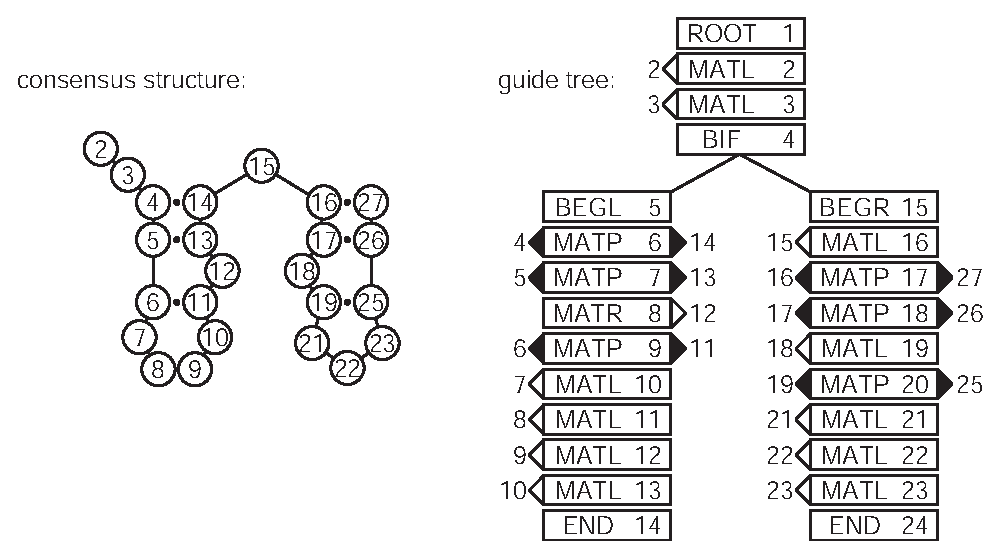
\includegraphics[width=5in]{Figures/cm_nodetree}
\end{center}
\caption{\small\textbf{The structural alignment is converted to a guide
tree.} Left: the consensus secondary structure is derived from the
annotated alignment in Figure~\ref{fig:input_alignment}. Numbers in
the circles indicate alignment column coordinates: e.g.  column 4 base
pairs with column 14, and so on. Right: the CM guide tree
corresponding to this consensus structure. The nodes of the tree are
numbered 1..24 in preorder traversal (see text). MATP, MATL, and MATR
nodes are associated with the columns they generate: e.g., node 6 is a
MATP (pair) node that is associated with the base-paired columns 4 and
14.}
\label{fig:cm_nodetree}
\end{figure}

Given the consensus structure, consensus base pairs are assigned to
MATP nodes and consensus unpaired columns are assigned to MATL or MATR
nodes. One ROOT node is used at the head of the tree.  Multifurcation
loops and/or multiple stems are dealt with by assigning one or more
BIF nodes that branch to subtrees starting with BEGL or BEGR head
nodes. (ROOT, BEGL, and BEGR start nodes are labeled differently
because they will be expanded to different groups of states; this has
to do with avoiding ambiguous parse trees for individual sequences, as
described below.) Alignment columns that are considered to be
insertions relative to the consensus structure are ignored at this
stage.

In general there will be more than one possible guide tree for any
given consensus structure. Almost all of this ambiguity is eliminated
by three conventions: (1) MATL nodes are always used instead of MATR
nodes where possible, for instance in hairpin loops; (2) in describing
interior loops, MATL nodes are used before MATR nodes; and (3) BIF
nodes are only invoked where necessary to explain branching secondary
structure stems (as opposed to unnecessarily bifurcating in single
stranded sequence). One source of ambiguity remains. In invoking a
bifurcation to explain alignment columns $i..j$ by two substructures
on columns $i..k$ and $k+1..j$, there will be more than one possible
choice of $k$ if $i..j$ is a multifurcation loop containing three or
more stems. The choice of $k$ impacts the performance of the divide
and conquer algorithm; for optimal time performance, we will want
bifurcations to split into roughly equal sized alignment problems, so
I choose the $k$ that makes $i..k$ and $k+1..j$ as close to the same
length as possible.

The result of this procedure is the guide tree. The nodes of the guide
tree are numbered in preorder traversal (e.g. a recursion of ``number
the current node, visit its left child, visit its right child'': thus
parent nodes always have lower indices than their children). The guide
tree corresponding to the input multiple alignment in
Figure~\ref{fig:input_alignment} is shown in
Figure~\ref{fig:cm_nodetree}.

\subsubsection{From guide tree to covariance model}

A CM must deal with insertions and deletions in individual sequences
relative to the consensus structure. For example, for a consensus base
pair, either partner may be deleted leaving a single unpaired residue,
or the pair may be entirely deleted; additionally, there may be
inserted nonconsensus residues between this pair and the next pair in
the stem. Accordingly, each node in the master tree is expanded into
one or more \emph{states} in the CM as follows:

\vspace{0.5em}
\begin{center}
\begin{tabular}{llccc}
       &                     & total \#& \# of split& \# of insert\\
Node   &  States             & states  & states     & states \\ \hline
MATP   & [MP ML MR D] IL IR  &   6     &   4        &  2   \\
MATL   & [ML D] IL           &   3     &   2    &  1   \\
MATR   & [MR D] IR           &   3     &   2    &  1   \\
BIF    & [B]                 &   1     &   1    &  0   \\
ROOT   & [S] IL IR           &   3     &   1    &  2   \\
BEGL   & [S]                 &   1     &   1    &  0   \\
BEGR   & [S] IL              &   2     &   1    &  1   \\
END    & [E]                 &   1     &   1    &  0   \\ \hline
\end{tabular}
\end{center}
\vspace{0.5em}

Here we distinguish between consensus (``M'', for ``match'') states
and insert (``I'') states. ML and IL, for example, are both L type
states with L type productions, but they will have slightly different
properties, as described below.

The states are grouped into a \emph{split set} of 1-4 states (shown in
brackets above) and an \emph{insert set} of 0-2 insert states. The
split set includes the main consensus state, which by convention is
first. One and only one of the states in the split set must be visited
in every parse tree (and this fact will be exploited by the divide and
conquer algorithm). The insert state(s) are not obligately visited,
and they have self-transitions, so they will be visited zero or more
times in any given parse tree.

State transitions are then assigned as follows. For bifurcation nodes,
the B state makes obligate transitions to the S states of the child
BEGL and BEGR nodes. For other nodes, each state in a split set has a
possible transition to every insert state in the \emph{same} node, and
to every state in the split set of the \emph{next} node. An IL state
makes a transition to itself, to the IR state in the same node (if
present), and to every state in the split set of the next node. An IR
state makes a transition to itself and to every state in the split set
of the next node.

There is one exception to this arrangement of transitions: insert
states that are immediately before an END node are effectively
\emph{detached} from the model by making transitions into them
impossible. This inelegant solution was imposed on the CM model
building procedure to fix a design flaw that allowed an ambiguity in
the determination of a parsetree given a structure. The detachment of
these special insert states removes this ambiguity.

This arrangement of transitions guarantees that (given the guide tree)
there is unambiguously one and only one parse tree for any given
individual structure. This is important. The algorithm will find a
maximum likelihood parse tree for a given sequence, and we wish to
interpret this result as a maximum likelihood structure, so there must
be a one to one relationship between parse trees and secondary
structures \citep{Giegerich00}.

The final CM is an array of $M$ states, connected as a directed graph
by transitions $t_v(y)$ (or probability 1 transitions $v \rightarrow
(y,z)$ for bifurcations) with the states numbered such that $(y,z)
\geq v$. There are no cycles in the directed graph other than cycles
of length one (e.g. the self-transitions of the insert states). We can
think of the CM as an array of states in which all transition
dependencies run in one direction; we can do an iterative dynamic
programming calculation through the model states starting with the
last numbered end state $M$ and ending in the root state $1$.  An
example CM, corresponding to the input alignment of
Figure~\ref{fig:input_alignment}, is shown in
Figure~\ref{fig:cm_graph}.

As a convenient side effect of the construction procedure, it is
guaranteed that the transitions from any state are to a
\emph{contiguous} set of child states, so the transitions for state
$v$ may be kept as an offset and a count. For example, in
Figure~\ref{fig:cm_graph}, state 12 (an MP) connects to states 16, 17,
18, 19, 20, and 21. We can store this as an offset of 4 to the first
connected state, and a total count of 6 connected states.  We know
that the offset is the distance to the next non-split state in the
current node; we also know that the count is equal to the number of
insert states in the current node, plus the number of split set states
in the next node. These properties make establishing the connectivity
of the CM trivial. Similarly, all the parents of any given state are
also contiguously numbered, and can be determined analogously. We are
also guaranteed that the states in a split set are numbered
contiguously.  This contiguity is exploited by the divide and conquer
implementation.

\begin{figure}[tp]
\begin{center}
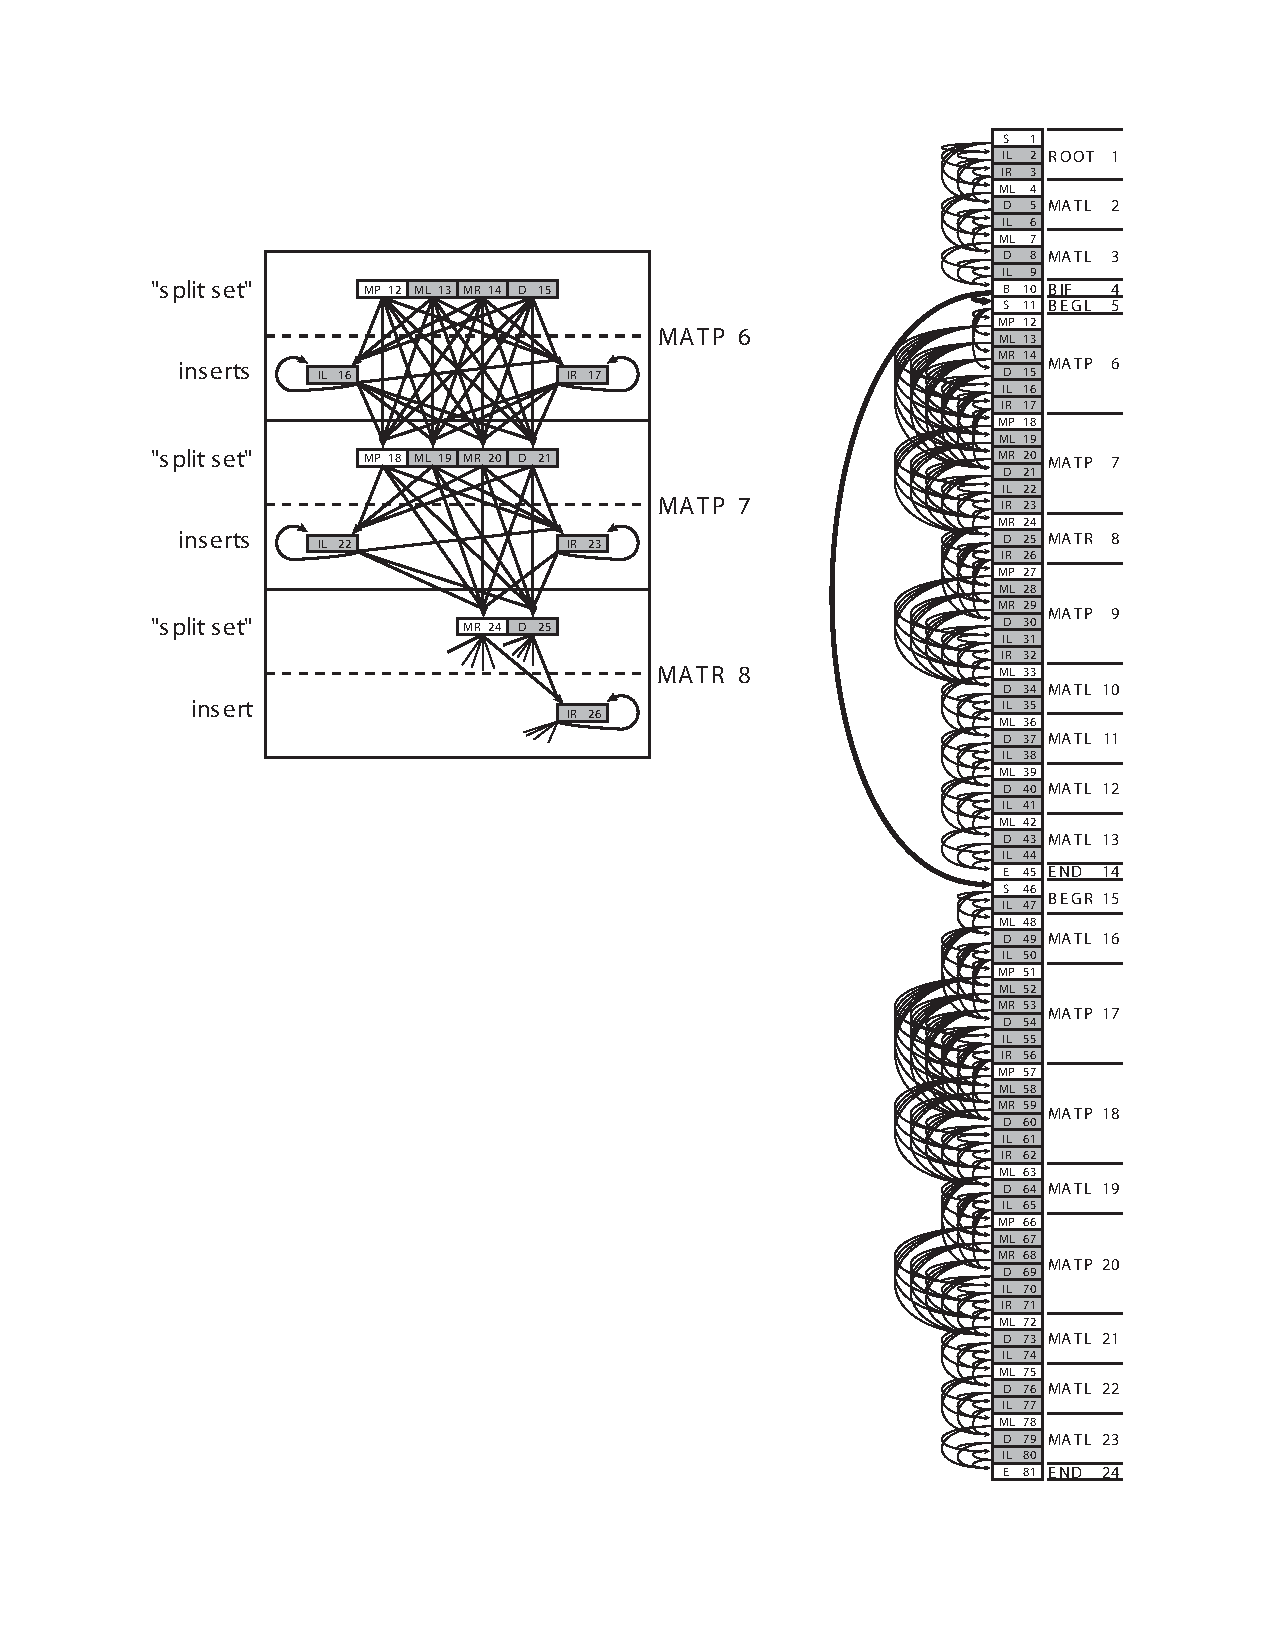
\includegraphics[width=5in]{Figures/cm_graph}
\end{center}
\caption{\small\textbf{A complete covariance model.} Right: the CM
corresponding to the alignment in Figure~\ref{fig:input_alignment}.
The model has 81 states (boxes, stacked in a vertical array). Each
state is associated with one of the 24 nodes of the guide tree (text
to the right of the state array). States corresponding to the
consensus are in white. States responsible for insertions and
deletions are gray. The transitions from bifurcation state B10 to
start states S11 and S46 are in bold because they are special: they
are an obligate (probability 1) bifurcation. All other transitions
(thin arrows) are associated with transition probabilities.  Emission
probability distributions are not represented in the figure. Left: the
states are also arranged according to the guide tree. A blow up of
part of the model corresponding to nodes 6, 7, and 8 shows
more clearly the logic of the connectivity of transition probabilities
(see main text), and also shows why any parse tree must transit through
one and only one state in each ``split set''.}
\label{fig:cm_graph}
\end{figure}

\subsubsection{Parameterization}

Using the guide tree and the final CM, each individual sequence in the
input multiple alignment can be converted unambiguously to a CM parse
tree, as shown in Figure~\ref{fig:parsetrees}. Weighted counts for
observed state transitions and singlet/pair emissions are then
collected from these parse trees. These counts are converted to
transition and emission probabilities, as maximum \emph{a posteriori}
estimates using mixture Dirichlet priors
\citep{Sjolander96,Durbin98,NawrockiEddy07}. 

\begin{figure}[t]
\begin{center}
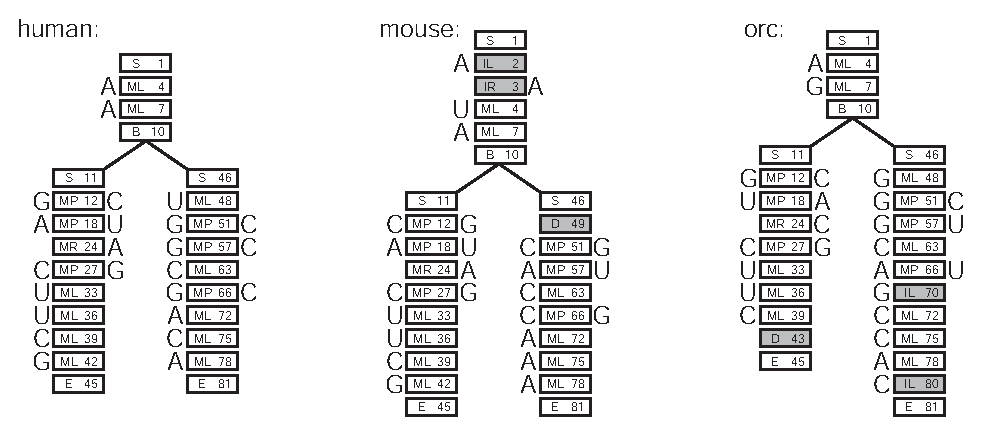
\includegraphics[width=5in]{Figures/parsetrees}
\end{center}
\caption{\small\textbf{Example parse trees.} Parse trees are shown for the
three sequences/structures from Figure~\ref{fig:input_alignment},
given the CM in Figure~\ref{fig:cm_graph}. For each sequence, each
residue must be associated with a state in the parse tree. (The
sequences can be read off its parse tree by starting at the upper left
and reading counterclockwise around the edge of parse tree.) Each
parse tree corresponds directly to a secondary structure -- base pairs
are pairs of residues aligned to MP states. A collection of parse
trees also corresponds to a multiple alignment, by aligning residues
that are associated with the same state -- for example, all three
trees have a residue aligned to state ML4, so these three residues
would be aligned together. Insertions and deletions relative to the
consensus use nonconsensus states, shown in gray.}
\label{fig:parsetrees}
\end{figure}

\subsubsection{Comparison to profile HMMs}

The relationship between an SCFG and a covariance model is analogous
to the relationship of hidden Markov models (HMMs) and profile HMMs
for modeling multiple sequence alignments
\citep{Krogh94,Durbin98,Eddy98}. A comparison may be instructive to
readers familiar with profile HMMs.  A profile HMM is a repetitive HMM
architecture that associates each consensus column of a multiple
alignment with a single type of model node -- a MATL node, in the
above notation. Each node contains a ``match'', ``delete'', and
``insert'' HMM state -- ML, IL, and D states, in the above notation.
The profile HMM also has special begin and end states. Profile HMMs
could therefore be thought of as a special case of CMs. An
unstructured RNA multiple alignment would be modeled by a guide tree
of all MATL nodes, and converted to an unbifurcated CM that would
essentially be identical to a profile HMM. (The only difference is
trivial; the CM root node includes a IR state, whereas the start node
of a profile HMM does not.) All the other node types (especially MATP,
MATR, and BIF) and state types (e.g. MP, MR, IR, and B) are SCFG
augmentations necessary to extend profile HMMs to deal with RNA
secondary structure.


\subsection{The \prog{cmbuild} program, step by step}
%\addtocontents{faq}{\textbf{Questions about using cmbuild:}}

The \prog{cmbuild} command line syntax is:

\user{cmbuild <options> [cmfile] [alifile]}

where \prog{[alifile]} is the name of the input alignment file, and
\prog{[cmfile]} is the name of the output CM file. What follows
describes the steps that \prog{cmbuild} goes through, and the most
important options that can be chosen to affect its behavior.

\subsubsection{Alignment input file}

The input alignment file must be in Stockholm format, and it must have
a consensus secondary structure annotation line (\otext{\#=GC SS\_cons}).

The program is actually capable of reading many common multiple
alignment formats (ClustalW, PHYLIP, GCG MSF, and others) but no other
format currently supports consensus RNA secondary structure
annotation. This may change in the future, either when other formats
allow structure annotation, or when \prog{cmbuild} is capable of
inferring consensus structure from the alignment by automated
comparative analysis, as the earlier COVE suite was capable
of \citep{Eddy94}. 

If the file does not exist, is not readable, or is not in a recognized
format, the program exits with a ``Alignment file doesn't exist or is
not readable'' error. If the file does not have consensus secondary
structure annotation, the program exits with a ``no consensus
structure annotation'' error. This includes all non-Stockholm
alignment files.

% EPN, Wed Apr  2 12:47:54 2008, the cat my.sto | cmbuild command
% in this faq no longer works.
\begin{srefaq}{Why does \prog{cmbuild} have a \prog{--informat} option, if it only
accepts Stockholm?} If you don't specify \prog{--informat}, the
software has to autodetect the file format. Autodetection of file
formats doesn't work in certain advanced/nonstandard cases, for
instance if you're reading the alignment from standard input instead
of from a file. The \prog{--informat} allows you to override
autodetection; e.g. \prog{cat my.sto | cmbuild --informat Stockholm
my.cm -} is an example of reading the alignment from piped standard
input.
\end{srefaq}

\subsubsection{Parsing secondary structure annotation}

The structure annotation line only needs to indicate which columns are
base paired to which. It does not have to be in full WUSS notation.
Even if it is, the details of the notation are largely ignored.
Nested pairs of \otext{<>}, \otext{()}, \otext{[]}, or \otext{{}} symbols
are interpreted as base paired columns. All other columns marked with
the symbols \otext{:,\_-.~} are interpreted as single stranded columns.

A simple minimal annotation is therefore to use \otext{<>} symbols to
mark base pairs and \otext{.} for single stranded columns.

If a secondary structure annotation line is in WUSS notation and it
contains valid pseudoknot annotation (e.g.\ additional non-nested
stems marked with AAA,aaa or BBB,bbb, etc.), this annotation is
ignored because Infernal cannot handle
pseudoknots. Internally, these columns are treated as if they were
marked with \otext{.} symbols.

\begin{srefaq}{How should I choose to annotate pseudoknots?} 
Infernal can only deal with nested base pairs. If there is
a pseudoknot, you have to make a choice of which stem to annotate as
normal nested structure (thus including it in the model) and which
stem to call additional ``pseudoknotted'' structure (thus ignoring it
in the model). For example, for a simple two-stem pseudoknot, should
you annotate it as \otext{AAAA.<<<<aaaa....>>>>}, or
\otext{<<<<.AAAA>>>>....aaaa}?  From an RNA structure viewpoint, which
stem I label as the pseudoknotted one is an arbitrary choice; but
since one of the stems in the pseudoknot will have to be modeled as a
single stranded region by Infernal, the choice makes a
slight difference in the performance of your model. You want your
model to capture as much information content as possible.  Thus, since
the information content of the model is a sum of the sequence
conservation plus the additional information contributed by pairwise
correlations in base-paired positions, you should tend to annotate the
shorter stem as the ``pseudoknot'' (modeling as many base pairs as
possible), and you should also annotate the stem with the more
conserved primary sequence as the ``pseudoknot'' (if one stem is more
conserved at the sequence level, you won't lose as much by modeling
that one as primary sequence consensus only).
\end{srefaq}

If (aside from any ignored pseudoknot annotation) the structure
annotation line contains characters other than \otext{<>()[]{}:\_-,.~}
then those characters are ignored (treated as \otext{.}) and a warning
is printed.

If, after this ``data cleaning'', the structure annotation is
inconsistent with a secondary structure (for example, if the number of
\otext{<} and \otext{>} characters isn't the same), then the program
exits with a ``failed to parse consensus structure annotation'' error.

\subsubsection{Sequence weighting}

By default, the input sequences are weighted in two ways to compensate
for biased sampling (phylogenetic correlations).  Relative sequence
weights are calculated by the Henikoff position-based method.
\citep{Henikoff94b}.  (The \prog{--wpb} option forces position-based
weights, but is redundant since that's the default.)  To turn relative
weighting off (e.g. set all weights to 1.0), use the \prog{--wnone}
option.

Some alignment file formats allow relative sequence weights to be
given in the file. This includes Stockholm format, which has
\otext{\#=GS WT} weight annotations. Normally \prog{cmbuild} ignores any
such input weights.  The \prog{--wgiven} option tells \prog{cmbuild}
to use them.  This lets you set the weights with any external
procedure you like; for example, the \prog{esl-weight} utility program in
Easel\footnote{This program will be in
  \ccode{infernal/easel/miniapps/} after building Infernal.} 
implements some common weighting algorithms,
including the Gerstein/Sonnhammer/Chothia weighting scheme
\citep{Gerstein94}.

Absolute weights (the ``effective sequence number'') is calculate by
``entropy weighting'' \citep{Karplus98}. This sets the balance between
the prior and the data, and affects the information content of the
model. Entropy weighting reduces the effective sequence number (the
total sum of the weights) and increases the entropy (degrading the
information content) of the model until a threshold is reached. The
default entropy is 1.41 bits per position (roughly 0.59 bits of
information, relative to uniform base composition). This threshold can
be changed with the \prog{--ere <x>} option. Entropy weighting may
be turned off entirely with the \prog{--enone} option.


\subsubsection{Architecture construction}

The CM architecture is now constructed from your input alignment and
your secondary structure annotation, as described in the previous
section. 

The program needs to determine which columns are consensus (match)
columns, and which are insert columns. (Remember that although WUSS
notation allows insertions to be annotated in the secondary structure
line, \prog{cmbuild} is only paying attention to annotated base
pairs.) By default, it does this by a simple rule based on the
frequency of residues (non-gaps) in a column. If the frequency of
residues is lower than a threshold, the column is considered to be
an insertion. Importantly though this frequency is determined using
the relative weights from the sequence weighting step, instead of
absolute gaps (e.g. a residue in a sequence with weight $0.8$ will count
 as $0.8$ residues).

The threshold defaults to 0.5. It can be changed to another number
\otext{<x>} (from 0 to 1.0) by the \prog{--symfrac <x>} option.  The
lower the number, the more columns are included in the model.  At
\prog{--symfrac 0.0}, all the columns are considered to be part of
the consensus. At \prog{--symfrac 1.0}, only columns with no gaps are.

You can also manually specify which columns are consensus versus
insert by including reference coordinate annotation (e.g. a
\otext{\#=GC RF} line, in Stockholm format) and using the
\prog{--hand} option. There's an example of this in the tutorial. Any
columns marked by non-gap symbols become consensus columns. (The
simplest thing to do is mark consensus columns with x's, and insert
columns with \otext{.}'s. Remember that spaces aren't allowed in
alignments in Stockholm format.) If you set the \prog{--hand} option but
your file doesn't have reference coordinate annotation, the program
exits with an error.

\subsubsection{Parameterization}

Weighted observed emission and transition counts are then collected
from the alignment data. These count vectors $c$ are then converted to
estimated probabilities $p$ using mixture Dirichlet priors
\citep{Sjolander96, Durbin98, NawrockiEddy07}. You can provide your
own prior as a file, using the \prog{--prior <f>} option.

As an exception, insert state emission probabilities are not learned
from the counts from implicit parse trees of sequences in the input
alignment, instead they are all set to 0.25 for each of the four RNA
nucleotides.  Another exception is made for transition counts in
ROOT\_IL and ROOT\_IR states from the implicit parsetrees. Any
transition counts in these states are \emph{ignored} by the
construction procedure -- they are set to zero before the transition
probability parameters for these states are determined.

\subsubsection{Naming the model}

Each CM gets a name. Stockholm format allows the alignment to have a
name, provided in the \otext{\#=GF ID} tag. If this name is provided,
it is used as the CM name.

Stockholm format allows more than one alignment per file, and
\prog{cmbuild} supports this: CM files can contain more than one
model, and if you say e.g.\ \prog{cmbuild Rfam.cm Rfam.sto} where
\otext{Rfam.sto} contains a whole database of alignments,
\prog{cmbuild} will create a database of CMs in the \prog{Rfam.cm} file,
one per alignment. 

If a name is not provided in the Stockholm \otext{\#=GF ID}
annotation, the name given to each CM is the input filename. This will
not work if the alignment file has more than one alignment. In that
case, you must include names for each alignment.

If the alignment file only has 1 alignment in it, you can override the
automatic naming conventions and provide your own name with the \prog{-n <s>}
option, where \prog{<s>} is any string. 

\subsubsection{Saving the model}

The model is now saved to a file, according to the filename specified
on the command line. By default, a new file is created, and the model
is saved in a portable ASCII text format. This format is described in
section~\ref{section:formats} of this guide.

If the cmfile already exists, the program exits with an error. The
\prog{-F} option causes the new model to overwrite an existing
cmfile. 




\newpage
\section{Tabular output formats}
\label{section:tabular}
\setcounter{footnote}{0}

\subsection{Target hits tables}

The \ccode{--tblout} output option in \prog{cmsearch} and
\prog{cmscan} produces \emph{target hits tables}. There are two
different formats of target hits table, which are both described
below. By default, both \prog{cmsearch} and \prog{cmscan} produce the
target hits table in \emph{format 1}. Format 1 is the only format that
was used by Infernal versions 1.1rc1 through 1.1.1. As of version 1.1.2,
with \prog{cmscan}, the \ccode{--fmt 2} option can be used in
combination with \ccode{--tblout} to produce a target hits table in
the alternative \emph{format 2}.  Both formats 1 and 2 target hits
table consist of one line for each different query/target comparison
that met the reporting thresholds, ranked by decreasing statistical
significance (increasing E-value).

\subsubsection{Target hits table format 1}

In the format 1 table, each line
consists of \textbf{18 space-delimited fields} followed by a free text
target sequence description, as follows:\footnote{The \ccode{tblout}
  format is deliberately space-delimited (rather than tab-delimited)
  and justified into aligned columns, so these files are suitable both
  for automated parsing and for human examination. Tab-delimited data
  files are difficult for humans to examine and spot check. For this
  reason, we think tab-delimited files are a minor evil in the
  world. Although we occasionally receive shrieks of outrage about
  this, we stubbornly feel that space-delimited files are just as
  trivial to parse as tab-delimited files.}

\begin{description}
\item[\emprog{(1) target name:}]
  The name of the target sequence or profile. 

\item[\emprog{(2) accession:}]
  The accession of the target sequence or profile, or '-' if none.

\item[\emprog{(3) query name:}] 
  The name of the query sequence or profile.

\item[\emprog{(4) accession:}]
  The accession of the query sequence or profile, or '-' if none.

\item[\emprog{(5) mdl (model):}] Which type of model was used to
  compute the final score. Either 'cm' or 'hmm'. A CM is
  used to compute the final hit scores unless the model has zero
  basepairs or the \ccode{--hmmonly} option is used, in which case a
  HMM will be used. 

\item[\emprog{(6) mdl from (model coord):}]
  The start of the alignment of this hit with respect to the
  profile (CM or HMM), numbered 1..N for a profile of N consensus positions.

\item[\emprog{(7) mdl to (model coord):}]
  The end of the alignment of this hit with respect to the
  profile (CM or HMM), numbered 1..N for a profile of N consensus positions.

\item[\emprog{(8) seq from (ali coord):}]
  The start of the alignment of this hit with respect to the
  sequence, numbered 1..L for a sequence of L residues.
 
\item[\emprog{(9) seq to (ali coord):}]
  The end of the alignment of this hit with respect to the
  sequence, numbered 1..L for a sequence of L residues.

\item[\emprog{(10) strand:}]
  The strand on which the hit occurs on the sequence. '+' if the hit is on
  the top (Watson) strand, '-' if the hit is on the bottom (Crick) strand.
  If on the top strand, the ``seq from'' value will be less than or
  equal to the ``seq to'' value, else it will be greater than or equal
  to it. 

\item[\emprog{(11) trunc:}] 
  Indicates if this is predicted to be a truncated CM hit or not. This will be
  ``no'' if it is a CM hit that is not predicted to be truncated by the end of the
  sequence, ``5'\,'' or ``3'\,'' if the hit is predicted to have one or more
  5' or 3' residues missing  due to a artificial truncation of the
  sequence, or ``5'\&3''' if the hit is predicted to have one or more
  5' residues missing and one or more 3' residues missing.
  If the hit is an HMM hit, this will always be '-'. 

\item[\emprog{(12) pass:}] 
  Indicates what ``pass'' of the pipeline the hit was detected
  on. This is probably only useful for testing and
  debugging. Non-truncated hits are found on the first pass, truncated
  hits are found on successive passes.

\item[\emprog{(13) gc:}] 
  Fraction of G and C nucleotides in the hit. 

\item[\emprog{(14) bias:}] The biased-composition correction: the bit
  score difference contributed by the null3 model for CM hits, or the
  null2 model for HMM hits. High bias scores may be a red flag for a
  false positive. It is difficult to correct for all possible ways in
  which a nonrandom but nonhomologous biological sequences can appear
  to be similar, such as short-period tandem repeats, so there are
  cases where the bias correction is not strong enough (creating false
  positives).

\item[\emprog{(15) score:}]
  The score (in bits) for this target/query comparison. It includes
  the biased-composition correction (the ``null3'' model for CM hits,
  or the ``null2'' model for HMM hits). 

\item[\emprog{(16) E-value:}] The expectation value (statistical
  significance) of the target.  This is a \emph{per query} E-value;
  i.e.\ calculated as the expected number of false positives achieving
  this comparison's score for a \emph{single} query against the search
  space $Z$. For \prog{cmsearch} $Z$ is defined as the total number of
  nucleotides in the target dataset multiplied by 2 because both strands
  are searched. For \prog{cmscan} $Z$ is the total number of
  nucleotides in the query sequence multiplied by 2 because both
  strands are searched and multiplied by the number of models in the target
  database. If you search with multiple queries and if you want to
  control the \emph{overall} false positive rate of that search rather
  than the false positive rate per query, you will want to multiply
  this per-query E-value by how many queries you're doing.

\item[\emprog{(17) inc:}] 
  Indicates whether or not this hit achieves the inclusion threshold:
  '!' if it does, '?' if it does not (and rather only achieves the
  reporting threshold). By default, the inclusion threshold is an
  E-value of 0.01 and the reporting threshold is an E-value of 10.0,
  but these can be changed with command line options as described in
  the manual pages.

\item[\emprog{(18) description of target:}] 
  The remainder of the line is the target's description line, as free text.
\end{description}

\subsubsection{Target hits table format 2}
\label{tabular-format2}

Format 2 includes all 18 of the fields from format 1 in the same order, plus 9
additional fields that are interspersed between some of the 18 from
format 1, as follows:

\begin{description}

\item[\emprog{(Before field 1 of format 1) idx:}] 
  The index of the hit in the list. The first hit has index '1', the
  second has index '2', the Nth hit has index 'N'.

\item[\emprog{(Before field 5 of format 1) clan name:}] 
  The name of the clan the model for this hit belongs to, or \ccode{-} if
  the model does not belong to a clan. A clan is a group of related
  models. For example, Rfam groups three LSU rRNA models
  (LSU\_rRNA\_archaea, LSU\_rRNA\_bacteria, and LSU\_rRNA\_eukarya)
  into the same clan. The value in this field will always be \ccode{-}
  unless the \ccode{--clanin <f>} option was used with
  \ccode{cmscan} to specify clan/model relationships in the input file
  \ccode{<f>}. See section~\ref{section:formats} for a description of
  the format of the input file used with \ccode{--clanin}.

\end{description}

The following seven fields all occur in format 2 between fields 17
('inc:') and 18 ('description of target') from format 1. 

\begin{description}

\item[\emprog{olp:}] A single character indicating the overlap status
  of this hit. Here, two hits are deemed to \emph{overlap} if they
  share at least one nucleotide on the same strand of the same
  sequence. There are three possible values in this field: \ccode{*},
  \ccode{\^} and \ccode{=}.  \ccode{*} indicates this hit does not
  overlap with any other reported hits. \ccode{\^} indicates that this
  hit does overlap with at least one other hit, but none of the hits
  that overlap with it have a higher score (occur above it in the hit
  list). \ccode{=} indicates that this hit does overlap with at least
  one other hit that has a higher score (occurs above it in the hit
  list). If the \ccode{--oclan} option was enabled, the definition of
  \emph{overlap} for the designations of the three characters
  \ccode{*}, \ccode{\^} and \ccode{=} described above changes to: two
  hits are deemed to \emph{overlap} if they share at least one
  nucleotide on the same strand of the same sequence and they are to
  models that are in the same clan. That is, only overlaps between
  hits to models that are in the same clan are counted, all other
  overlaps are ignored and not annotated.  Infernal will never report
  two overlapping hits to the same model.

\item[\emprog{anyidx:}]
For hits that have \ccode{=} in the ``olp'' field, this is the
index of the best scoring hit that overlaps with this hit.
For hits with either \ccode{*} or \ccode{\^} in the "olp" field,
this field will always be \ccode{-}.

\item[\emprog{anyfrct1:}]
For hits that have \ccode{=} in the "olp" field, this is the
fraction of the length of this hit that overlaps with the best scoring
overlapping hit (the hit index given in the "anyidx" field), to
4 significant digits. 
For hits with \ccode{-} in the "anyidx"
field, this field will always be \ccode{-}.  

\item[\emprog{anyfrct2:}]
For hits that have \ccode{=} in the "olp" field, this is the
fraction of the length of the best scoring overlapping hit (the hit
index given in the "anyidx" field) that overlaps with this hit,
to 4 significant digits. 
For hits with \ccode{-} in the "anyidx"
field, this field will always be \ccode{-}.  

\item[\emprog{winidx:}] 
For hits that have \ccode{=} in the "olp" field, this is either
\ccode{"} or the index of the best scoring hit that overlaps with this
hit that is marked as \ccode{\^} in the "olp" field. If the value
is \ccode{"} it means that the best scoring hit that overlaps with
this hit that is marked as \ccode{\^} in the "olp" field is
already listed in the "anyidx" field, which is usually the case.
For hits with either \ccode{*} or \ccode{\^} in the "olp" field,
this field will always be \ccode{-}.

\item[\emprog{winfrct1:}]
For hits that have neither \ccode{-} nor \ccode{"} in the
"winidx" field, this is the fraction of the length of this hit
that overlaps with the best scoring overlapping hit marked with
\ccode{\^} in the "olp" field (the hit index given in the
"winidx" field), to 4 significant digits.  For hits with either
\ccode{*} or \ccode{\^} in the "olp" field, this field will
always be \ccode{-}.  For hits with \ccode{-} in the "winidx"
field, this field will always be \ccode{-}.  
For hits with \ccode{"} in the "winidx"
field, this field will always be \ccode{"}.  

\item[\emprog{winfrct2:}]
For hits that have neither \ccode{-} nor \ccode{"} in the
"winidx" field, this is the
fraction of the length of the best scoring overlapping hit marked with
\ccode{\^} in the "olp" field (the hit
index given in the "winidx" field) that overlaps with this hit,
to 4 significant digits. 
  For hits with either
\ccode{*} or \ccode{\^} in the "olp" field, this field will
always be \ccode{-}.  For hits with \ccode{-} in the "winidx"
field, this field will always be \ccode{-}.  
For hits with \ccode{"} in the "winidx"
field, this field will always be \ccode{"}.  

\end{description}

The tables are columnated neatly for human readability, but do not
write parsers that rely on this columnation; rely on space-delimited
fields. The pretty columnation assumes fixed maximum widths for each
field. If a field exceeds its allotted width, it will still be fully
represented and space-delimited, but the columnation will be disrupted
on the rest of the row.

Note the use of target and query columns. A program like
\prog{cmsearch} searches a query profile against a target sequence
database. In an \prog{cmsearch} tblout file, the sequence (target)
name is first, and the profile (query) name is second. A program like
\prog{cmscan}, on the other hand, searches a query sequence against a
target profile database. In a \prog{cmscan} tblout file, the profile
name is first, and the sequence name is second. You might say, hey,
wouldn't it be more consistent to put the profile name first and the
sequence name second (or vice versa), so \prog{cmsearch} and
\prog{cmscan} tblout files were identical? Well, they
still wouldn't be identical, because the target database size used for
E-value calculations is different (total number of target nucleotides
for \prog{cmsearch}, number of target profiles times target sequence
length for \prog{cmscan}), and it's good not to forget this.

If some of the descriptions of these fields don't make sense to you,
it may help to go through the tutorial in
section~\ref{section:tutorial} and read section~\ref{section:pipeline}
of the manual. 



% Changes in options between 1.0 and 1.1 are omitted from the 1.1.2 user guide.
%\newpage
%\section{Changes in command-line options from version 1.0}
\label{section:options}
\setcounter{footnote}{0}

The following tables list options from Infernal version 1.0 programs
that have either been removed, renamed or significantly changed in
version 1.1. Many options in cmsearch and cmcalibrate have changed or
been removed, mainly because the new search pipeline (see
section~\ref{section:pipeline}) is so different from the version 1.0
pipeline. For example the version 1.0 pipeline set HMM filter
thresholds for a search in a model-dependent manner, whereas those
thresholds are model-independent in version 1.1. Also, cmalign and
cmstat in version 1.1 are significantly simpler than they were in
version 1.0 and have many fewer options. The motivation for renaming
options whose behavior did not change was for consistency with
HMMER3, so that analogous options in Infernal and HMMER have the same
name. For more information on the version 1.1 options, see the manual
pages in this guide.

\subsection{cmalign options from Infernal version 1.0.x that have changed in version 1.1.} 

\begin{tabular}{|lll|}
\hline
%\multicolumn{3}{|l|}{\prog{cmalign} options in Infernal version 1.0 that have changed in version 1.1.} \\ \hline
                       & corresponding            &                                     \\
v1.0 option            & v1.1 option              & explanation                         \\ \hline
\otext{-1}             & \otext{--outformat pfam} & renamed only; no change in behavior \\
\otext{--banddump <n>} & none                     & no longer supported \\
\otext{--beta}         & none                     & QDB alignment is no longer supported \\
\otext{--checkfb}      & none                     & no longer supported \\
\otext{--checkpost}    & none                     & no longer supported \\
\otext{--devhelp}      & none                     & no longer necessary \\
\otext{--dlev}         & none                     & no longer supported \\
\otext{--dna}          & \otext{--dnaout}         & renamed only; no change in behavior \\
\otext{--fins}         & none                     & no longer supported \\
\otext{--gapthresh}    & none                     & no longer necessary \\
\otext{--hsafe}        & none                     & no longer supported \\
\otext{--inside}       & none                     & no longer supported \\
\otext{-l}             & none                     & true by default, local alignment is now the default behavior \\
none                   & \otext{-g}               & for global alignment, use \otext{-g} \\
\otext{--merge}        & none                     & no longer supported \\
\otext{--no-null3}     & none                     & no longer supported \\
\otext{--onepost}      & none                     & no longer supported \\
\otext{-p}             & none                     & true by default \\
none                   & \otext{--noprob}         & disable posterior probability annotation with \otext{--noprob} \\
\otext{-q}             & none                     & true by default, output scores with \otext{-o} or \otext{--sfile} \\
\otext{--qdb}          & none                     & QDB alignment is no longer supported \\
\otext{--pbegin <x>}   & none                     & no longer supported; settable for a CM in \otext{cmbuild} \\
\otext{--pebegin}      & none                     & no longer supported; settable for a CM in \otext{cmbuild} \\
\otext{--pend <x>}     & none                     & no longer supported; settable for a CM in \otext{cmbuild} \\
\otext{--pfend <x>}    & none                     & no longer supported; settable for a CM in \otext{cmbuild} \\
\otext{--resonly}      & none                     & no longer supported \\
\otext{--rf}           & none                     & no longer necessary \\
\otext{--rna}          & none                     & RNA output is true by default \\
\otext{-s}             & \otext{--seed}           & renamed only; no change in behavior \\
\otext{--sums}         & none                     & no longer supported \\
\otext{--viterbi}      & none                     & no longer supported \\
\otext{--withali <f>}  & \otext{--mapali <f>}     & \otext{<f>} must now be same alignment used to build CM \\
\otext{--withpknots}   & \otext{--withstr}        & renamed only; no change in behavior \\
\hline
\end{tabular}

\subsection{cmbuild options from Infernal version 1.0.x that have changed in version 1.1.} 

\begin{tabular}{|lll|}
\hline
%\multicolumn{3}{|l|}{\prog{cmalign} options in Infernal version 1.0 that have changed in version 1.1.} \\ \hline
                       & corresponding            &                                     \\
v1.0 option            & v1.1 option              & explanation                         \\ \hline
\otext{-a}             & \otext{--indi}           & renamed only; no change in behavior \\
\otext{-A}             & none                     & no longer supported \\
\otext{--eX}           & none                     & no longer supported \\
\otext{--gapthresh <x>}& \otext{--symfrac <y>}    & renamed; IMPORTANT: use \otext{<y>} equal to \otext{1.0-<x>} \\
                       &                          & where \otext{<x>} is from \otext{--gapthresh <x>} in v1.0 \\
\otext{--ignorant}     & \otext{--noss}           & renamed             \\
\otext{--pbswitch}     & none                     & no longer supported \\
\otext{-s}             & \otext{--seed}           & renamed only; no change in behavior \\
\otext{--rf}           & \otext{--hand}           & renamed only; no change in behavior \\
\otext{--regress}      & none                     & no longer supported \\
\otext{-v}             & \otext{--verbose}        & renamed             \\
\otext{--Wbeta <f>}    & \otext{--betaW}          & renamed only; no change in behavior \\
\hline
\end{tabular}


\subsection{cmcalibrate options from Infernal version 1.0.x that have changed in version 1.1.} 

\begin{tabular}{|lll|}
\hline
%\multicolumn{3}{|l|}{\prog{cmalign} options in Infernal version 1.0 that have changed in version 1.1.} \\ \hline
                             & corresponding            &                                     \\
v1.0 option                  & v1.1 option              & explanation                         \\ \hline
\otext{--devhelp}            & none                     & no longer necessary \\
\otext{--exp-beta <x>}       & \otext{--beta <x>}       & renamed only; no change in behavior \\
\otext{--exp-cmL-glc <x>}    & \otext{-L <x>}           & renamed \\
\otext{--exp-cmL-loc <x>}    & \otext{-L <x>}           & renamed \\
\otext{--exp-ffile <f>}      & \otext{--ffile <f>}      & renamed only; no change in behavior \\
\otext{--exp-fract}          & none                     & no longer relevant; HMMs are not calibrated \\
\otext{--exp-gc <f>}         & \otext{--gc}             & renamed only; no change in behavior \\
\otext{--exp-hfile <f>}      & \otext{--hfile <f>}      & renamed only; no change in behavior \\
\otext{--exp-hmmLn-glc <x>}  & none                     & no longer necessary; HMMs are not calibrated \\
\otext{--exp-hmmLn-loc <x>}  & none                     & no longer necessary; HMMs are not calibrated \\
\otext{--exp-hmmLx <x>}      & none                     & no longer necessary; HMMs are not calibrated \\
\otext{--exp-no-qdb}         & \otext{--noqdb}          & renamed only; no change in behavior \\
\otext{--exp-pfile <f>}      & none                     & no longer supported \\
\otext{--exp-qqfile <f>}     & \otext{--qqfile <f>}     & renamed only; no change in behavior \\
\otext{--exp-random}         & \otext{--random}         & renamed only; no change in behavior \\
\otext{--exp-sfile <f>}      & \otext{--sfile <f>}      & renamed only; no change in behavior \\
\otext{--exp-tailn-cglc}     & \otext{--gtailn}         & renamed \\
\otext{--exp-tailn-cloc}     & \otext{--ltailn}         & renamed \\
\otext{--exp-tailn-hglc <x>} & none                     & no longer necessary; HMMs are not calibrated \\
\otext{--exp-tailn-hloc <x>} & none                     & no longer necessary; HMMs are not calibrated \\
\otext{--exp-tailp}          & \otext{--tailp}          & renamed \\
\otext{--exp-tailxn}         & none                     & no longer supported \\
\otext{--exp-T <x>}          & none                     & no longer supported \\
\otext{--fil-aln2bands}      & none                     & no longer necessary; HMM filter thresholds no longer used \\
\otext{--fil-dfile}          & none                     & no longer necessary; HMM filter thresholds no longer used \\
\otext{--fil-gemit}          & none                     & no longer necessary; HMM filter thresholds no longer used \\
\otext{--fil-F <x>}          & none                     & no longer necessary; HMM filter thresholds no longer used \\
\otext{--fil-N <n>}          & none                     & no longer necessary; HMM filter thresholds no longer used \\
\otext{--fil-nonbanded}      & none                     & no longer necessary; HMM filter thresholds no longer used \\
\otext{--fil-Smax-hmm <x>}   & none                     & no longer necessary; HMM filter thresholds no longer used \\
\otext{--fil-Smin-hmm <x>}   & none                     & no longer necessary; HMM filter thresholds no longer used \\
\otext{--fil-Starg-hmm <x>}  & none                     & no longer necessary; HMM filter thresholds no longer used \\
\otext{--fil-tau <x>}        & none                     & no longer necessary; HMM filter thresholds no longer used \\
\otext{--fil-Xmin-hmm <x>}   & none                     & no longer necessary; HMM filter thresholds no longer used \\
\otext{--fil-Xtarg-hmm <x>}  & none                     & no longer necessary; HMM filter thresholds no longer used \\
\otext{--forecast <n>}       & \otext{--forecast}       & no longer takes \# of processors \otext{<n>}; use in combination\\
                             &                          & with \otext{--nforecast <n>} to reproduce v1.0 behavior \\
\otext{--mxsize}             & none                     & no longer supported \\
\otext{--no-null3}           & \otext{--nonull3}        & renamed only; no change in behavior \\
\otext{--pbegin <x>}         & none                     & no longer supported; settable for a CM in \otext{cmbuild} \\
\otext{--pebegin}            & none                     & no longer supported; settable for a CM in \otext{cmbuild} \\
\otext{--pend <x>}           & none                     & no longer supported; settable for a CM in \otext{cmbuild} \\
\otext{--pfend <x>}          & none                     & no longer supported; settable for a CM in \otext{cmbuild} \\
\otext{-s}                   & \otext{--seed}           & renamed only; no change in behavior \\
\otext{-v}                   & none                     & no longer supported \\
\hline
\end{tabular}


\subsection{cmemit options from Infernal version 1.0.x that have changed in version 1.1.} 

\begin{tabular}{|lll|}
\hline
%\multicolumn{3}{|l|}{\prog{cmalign} options in Infernal version 1.0 that have changed in version 1.1.} \\ \hline
                       & corresponding            &                                     \\
v1.0 option            & v1.1 option              & explanation                         \\ \hline
\otext{-n}             & \otext{-N}               & renamed only; no change in behavior \\
\otext{-s}             & \otext{--seed}           & renamed only; no change in behavior \\
\otext{--begin <n>}    & \otext{--a5p <n>}        & renamed only; no change in behavior \\
\otext{--end <n>}      & \otext{--a3p <n>}        & renamed only; no change in behavior \\
\otext{--shmm}         & none                     & no longer supported \\
\otext{--ahmm}         & none                     & no longer supported \\
\otext{--pbegin <x>}   & none                     & no longer supported; settable for a CM in \otext{cmbuild} \\
\otext{--pebegin}      & none                     & no longer supported; settable for a CM in \otext{cmbuild} \\
\otext{--pend <x>}     & none                     & no longer supported; settable for a CM in \otext{cmbuild} \\
\otext{--pfend <x>}    & none                     & no longer supported; settable for a CM in \otext{cmbuild} \\
\hline
\end{tabular}


\subsection{cmsearch options from Infernal version 1.0.x that have changed in version 1.1.} 

\begin{tabular}{|lll|}
\hline
%\multicolumn{3}{|l|}{\prog{cmalign} options in Infernal version 1.0 that have changed in version 1.1.} \\ \hline
                           & corresponding            &                                     \\
v1.0 option                & v1.1 option              & explanation                         \\ \hline
\otext{--aln2hbands}       & none                     & no longer supported \\
\otext{--aln-hbanded}      & none                     & true by default \\
\otext{--aln-optacc}       & none                     & true by default \\
\otext{--dna}              & none                     & no longer supported \\
\otext{--fil-no-hmm}       & \otext{--nohmm}          & renamed \\
\otext{--fil-no-qdb}       & \otext{--max}            & \otext{--max} turns off all filters \\
\otext{--fil-beta <x>}     & \otext{--fbeta <x>}      & renamed \\
\otext{--fil-A-hmm <x>}    & none                     & no longer supported \\
\otext{--fil-finE-hmm <x>} & none                     & no longer supported \\
\otext{--fil-finE-qdb <x>} & none                     & no longer supported \\
\otext{--fil-finT-hmm <x>} & none                     & no longer supported \\
\otext{--fil-finT-qdb <x>} & none                     & no longer supported \\
\otext{--fil-E-hmm <x>}    & none                     & no longer supported \\
\otext{--fil-E-qdb <x>}    & none                     & no longer supported \\
\otext{--fil-S-hmm <x>}    & none                     & no longer supported \\
\otext{--fil-Smax-hmm <x>} & none                     & no longer supported \\
\otext{--fil-Smin-hmm <x>} & none                     & no longer supported \\
\otext{--fil-T-hmm <x>}    & none                     & no longer supported \\
\otext{--fil-T-qdb <x>}    & none                     & no longer supported \\
\otext{--fil-Xmin-hmm <x>} & none                     & no longer supported \\
\otext{--forecast <n>}     & none                     & no longer supported \\
\otext{--forward}          & \otext{--hmmonly}        & renamed \\
\otext{--ga}               & \otext{--cut\_ga}        & renamed only; no change in behavior \\
\otext{--gcfile <f>}       & none                     & no longer supported \\
\otext{--hbanded}          & none                     & true by default \\
\otext{--hmm-W <n>}        & none                     & no longer supported \\
\otext{--hmm-cW <x>}       & \otext{--wcx <x>}        & renamed \\
\otext{--informat <s>}     & \otext{--tformat <s>}    & renamed only; no change in behavior \\
\otext{--inside}           & none                     & true by default \\
\otext{--lambda <x>}       & none                     & no longer supported \\
\otext{--nc}               & \otext{--cut\_nc}        & renamed only; no change in behavior \\
\otext{--noalign}          & \otext{--noali}          & renamed \\
\otext{--no-qdb}           & \otext{--nonbanded}      & renamed only; no change in behavior \\
\otext{--tabfile <f>}      & \otext{--tblout <f>}     & renamed, and format of \otext{<f>} changed \\
\otext{--tc}               & \otext{--cut\_tc}        & renamed only; no change in behavior \\
\otext{--no-null3}         & \otext{--nonull3}        & renamed only; no change in behavior \\
\otext{--null2}            & none                     & no longer supported \\
\otext{-p}                 & none                     & true by default \\
\otext{--pbegin <x>}       & none                     & no longer supported; settable for a CM in \otext{cmbuild} \\
\otext{--pebegin}          & none                     & no longer supported; settable for a CM in \otext{cmbuild} \\
\otext{--pend <x>}         & none                     & no longer supported; settable for a CM in \otext{cmbuild} \\
\otext{--pfend <x>}        & none                     & no longer supported; settable for a CM in \otext{cmbuild} \\
\otext{--rna}              & none                     & true by default \\
\otext{--rtrans}           & none                     & no longer supported \\
\otext{-v}                 & none                     & no longer supported \\
\otext{--viterbi}          & none                     & no longer supported \\
\otext{-x}                 & none                     & no longer supported \\
\hline
\end{tabular}


\subsection{cmstat options from Infernal version 1.0.x that have changed in version 1.1.} 

\begin{tabular}{|lll|}
\hline
%\multicolumn{3}{|l|}{\prog{cmalign} options in Infernal version 1.0 that have changed in version 1.1.} \\ \hline
                           & corresponding            &                                     \\
v1.0 option                & v1.1 option              & explanation                         \\ \hline
\otext{-g}                 & none                     & no longer relevant\\
\otext{-m}                 & none                     & true by default \\
\otext{--le}               & none                     & no longer supported \\
\otext{--ge}               & none                     & no longer supported \\
\otext{--beta <x>}         & none                     & no longer relevant \\
\otext{--qdbfile <x>}      & none                     & no longer supported \\
\otext{--lfi}              & none                     & no longer relevant \\
\otext{--gfi}              & none                     & no longer relevant \\
\otext{--lfc}              & none                     & no longer relevant \\
\otext{--gfc}              & none                     & no longer relevant \\
\otext{-E <x>}             & none                     & \otext{-E <x>} behaves differently now \\
\otext{-T <x>}             & none                     & \otext{-T <x>} behaves differently now \\
\otext{--nc}               & none                     & no longer relevant \\
\otext{--ga}               & none                     & no longer relevant \\
\otext{--tc}               & none                     & no longer relevant \\
\otext{--seqfile <f>}      & none                     & no longer supported \\
\otext{--toponly}          & none                     & no longer supported \\
\otext{--search}           & none                     & no longer supported \\
\otext{--cmL}              & none                     & no longer supported \\
\otext{--hmmL}             & none                     & no longer supported \\
\otext{--efile <f>}        & none                     & no longer relevant \\
\otext{--bfile <f>}        & none                     & no longer relevant \\
\otext{--sfile <f>}        & none                     & no longer relevant \\
\otext{--xfile <f>}        & none                     & no longer relevant \\
\otext{--afile <f>}        & none                     & no longer relevant \\
\otext{--bits}             & none                     & no longer relevant \\
\hline
\end{tabular}


\newpage

\section{Some other topics}
\label{section:more}
\setcounter{footnote}{0}

\subsection{How do I cite HMMER?}

The appropriate citation is to the web site, \url{hmmer.org}. You
should also cite what version of the software you used. We archive all
old versions, so anyone should be able to obtain the version you used,
when exact reproducibility of an analysis is an issue. 

The version number is in the header of most output files. To see it
quickly, do something like \prog{hmmscan -h} to get a help page, and
the header will say:

\begin{sreoutput}
# hmmscan :: search sequence(s) against a profile database
# HMMER 3.1 (February 2013); http://hmmer.org/
# Copyright (C) 2011 Howard Hughes Medical Institute.
# Freely distributed under the GNU General Public License (GPLv3).
# - - - - - - - - - - - - - - - - - - - - - - - - - - - - - - - - - - - -
\end{sreoutput}

So (from the second line there) this is from HMMER 3.1.

There is not yet any appropriate citable published paper that
describes the HMMER3 software suite.



\subsection{How do I report a bug?}

Email us, at \url{hmmer@janelia.hhmi.org}.

Before we can see what needs fixing, we almost always need to
reproduce a bug on one of our machines. This means we want to have a
small, reproducible test case that shows us the failure you're seeing.
So if you're reporting a bug, please send us:

\begin{itemize}
 \item A brief description of what went wrong.
 \item The command line(s) that reproduce the problem.
 \item Copies of any files we need to run those command lines.
 \item Information about what kind of hardware you're on, what
   operating system, and (if you compiled the software yourself rather
   than running precompiled binaries), what compiler and version you
   used, with what configuration arguments.
\end{itemize}

Depending on how glaring the bug is, we may not need all this
information, but any work you can put into giving us a clean
reproducible test case doesn't hurt and often helps.

The information about hardware, operating system, and compiler is
important. Bugs are frequently specific to particular configurations
of hardware/OS/compiler.  We have a wide variety of systems available
for trying to reproduce bugs, and we'll try to match your system as
closely as we can.

If you first see a problem on some huge compute (like running a
zillion query sequence over a huge profile database), it will really,
really help us if you spend a bit of time yourself trying to isolate
whether the problem really only manifests itself on that huge compute,
or if you can isolate a smaller test case for us. The ideal bug report
(for us) gives us everything we need to reproduce your problem in one
email with at most some small attachments. 

Remember, we're not a company with dedicated support staff -- we're a
small lab of busy researchers like you. Somebody here is going to drop
what they're doing to try to help you out. Try to save us some time,
and we're more likely to stay in our usual good mood.

If we're in our usual good mood, we'll reply quickly.  We'll probably
tell you we fixed the bug in our development code, and that the fix
will appear in the next HMMER release. This of course doesn't help you
much, since nobody knows when the next HMMER release is going to be.
So if possible, we'll usually try to describe a workaround for the
bug.

If the code fix is small, we might also tell you how to patch and
recompile the code yourself. You may or may not want to do this.


There are currently not enough open bugs to justify having a formal
on-line bug tracking system. We have a bugtracking system, but it's
internal.


\subsection{Input files}

\subsubsection{Reading from a stdin pipe using - (dash) as a filename argument}

Generally, HMMER programs read their sequence and/or profile input
from files. Unix power users often find it convenient to string an
incantation of commands together with pipes (indeed, such wizardly
incantations are a point of pride). For example, you might extract a
subset of query sequences from a larger file using a one-liner
combination of scripting commands (perl, awk, whatever). To facilitate
the use of HMMER programs in such incantations, you can almost always
use an argument of '-' (dash) in place of a filename, and the program
will take its input from a standard input pipe instead of opening a
file.

For example, the following three commands are entirely equivalent, and
give essentially identical output:

\user{hmmsearch globins4.hmm uniprot\_sprot.fasta} 

\user{cat globins4.hmm | hmmsearch - uniprot\_sprot.fasta}

\user{cat uniprot\_sprot.fasta | hmmsearch globins4.hmm - }

Most Easel ``miniapp'' programs share the same ability of pipe-reading.

Because the programs for profile HMM fetching (\prog{hmmfetch}) and
sequence fetching (\prog{esl-sfetch}) can fetch any number of profiles
or sequences by names/accessions given in a list, \emph{and} these
programs can also read these lists from a stdin pipe, you can craft
incantations that generate subsets of queries or targets on the
fly. For example:

\user{esl-sfetch --index uniprot\_sprot.fasta}

\user{cat mytargs.list | esl-sfetch -f uniprot\_sprot.fasta - | hmmsearch globins4.hmm -}

This takes a list of sequence names/accessions in
\prog{mytargets.list}, fetches them one by one from UniProt (note that
we index the UniProt file first, for fast retrieval; and note that
\prog{esl-sfetch} is reading its \prog{<namefile>} list of
names/accessions through a pipe using the '-' argument), and pipes
them to an \prog{hmmsearch}. It should be obvious from this that we
can replace the \prog{cat mytargets.list} with \emph{any} incantation
that generates a list of sequence names/accessions (including SQL
database queries).

Ditto for piping subsets of profiles. Supposing you have a copy of Pfam in Pfam-A.hmm:

\user{hmmfetch --index Pfam-A.hmm}

\user{cat myqueries.list | hmmfetch -f Pfam.hmm - | hmmsearch - uniprot\_sprot.fasta}

This takes a list of query profile names/accessions in
\prog{myqueries.list}, fetches them one by one from Pfam, and does an
hmmsearch with each of them against UniProt. As above, the \prog{cat
  myqueries.list} part can be replaced by any suitable incantation
that generates a list of profile names/accessions.

There are three kinds of cases where using '-' is restricted or
doesn't work. A fairly obvious restriction is that you can only use
one '-' per command; you can't do a \prog{hmmsearch - -} that tries to
read both profile queries and sequence targets through the same stdin
pipe. Second, another case is when an input file must be obligately
associated with additional, separately generated auxiliary files, so
reading data from a single stream using '-' doesn't work because the
auxiliary files aren't present (in this case, using '-' will be
prohibited by the program). An example is \prog{hmmscan}, which needs
its \prog{<hmmfile>} argument to be associated with four auxiliary
files named \prog{<hmmfile>.h3\{mifp\}} that \prog{hmmpress} creates,
so \prog{hmmscan} does not permit a '-' for its \prog{<hmmfile>}
argument. Finally, when a command would require multiple passes over
an input file, the command will generally abort after the first pass
if you are trying to read that file through a standard input pipe
(pipes are nonrewindable in general; a few HMMER or Easel programs
will buffer input streams to make multiple passes possible, but this
is not usually the case). An example would be trying to search a file
containing multiple profile queries against a streamed target
database:

\user{cat myqueries.list | hmmfetch -f Pfam.hmm > many.hmms}

\user{cat mytargets.list | esl-sfetch -f uniprot\_sprot.fasta - | hmmsearch many.hmms -}

This will fail. Unfortunately the above business about how it will
``generally abort after the first pass'' means it fails weirdly. The
first query profile search will succeed, and its output will appear;
then an error message will be generated when \prog{hmmsearch} sees the
\emph{second} profile query and oops, it realizes it is unable to
rewind the target sequence database stream. This is inherent in how it
reads the profile HMM query file sequentially as a stream (which is
what's allowing it to read input from stdin pipes in the first place),
one model at a time: it doesn't see there's more than one query model
in the file until it gets to the second model.

This case isn't too restricting because the same end goal can be
achieved by reordering the commands. In cases where you want to do
multiple queries against multiple targets, you always want to be
reading the \emph{queries} from a stdin pipe, not the targets:

\user{cat mytargets.list | esl-sfetch -f uniprot\_sprot.fasta > mytarget.seqs}

\user{cat myqueries.list | hmmfetch -f Pfam.hmm - |  hmmsearch - mytarget.seqs}

So in this multiple queries/multiple targets case of using stdin
pipes, you just have to know, for any given program, which file it
considers to be queries and which it considers to be targets. (That
is, the logic in searching many queries against many targets is ``For
each query: search the target database; then rewind the target
database to the beginning.'') For \prog{hmmsearch}, the profiles are
queries and sequences are targets. For \prog{hmmscan}, the reverse.

In general, HMMER and Easel programs document in their man page
whether (and which) command line arguments can be replaced by '-'.
You can always check by trial and error, too. The worst that can
happen is a ``Failed to open file -'' error message, if the program
can't read from pipes.




\newpage
\input{manpages}

\newpage
\section{File formats}
\label{section:formats}
\setcounter{footnote}{0}

\subsection{HMMER profile HMM files}
\label{section:savefiles}

The file \prog{tutorial/fn3.hmm} gives an example of a HMMER3 ASCII
save file. An abridged version is shown here, where (\ldots) mark
deletions made for clarity and space:

\begin{tinysreoutput}
HMMER3/f [3.1 | February 2013]
NAME  fn3
ACC   PF00041.13
DESC  Fibronectin type III domain
LENG  86
ALPH  amino
RF    no
MM    no
CONS  yes
CS    yes
MAP   yes
DATE  Fri Feb 15 06:04:13 2013
NSEQ  106
EFFN  11.415833
CKSUM 3564431818
GA    8.00 7.20
TC    8.00 7.20
NC    7.90 7.90
STATS LOCAL MSV       -9.4043  0.71847
STATS LOCAL VITERBI   -9.7737  0.71847
STATS LOCAL FORWARD   -3.8341  0.71847
HMM          A        C        D        E        F        G        H        I    (...)    Y   
            m->m     m->i     m->d     i->m     i->i     d->m     d->d
  COMPO   2.70330  4.91262  3.03272  2.64079  3.60307  2.84344  3.74204  3.07942 (...) 3.21526
          2.68618  4.42225  2.77519  2.73123  3.46354  2.40513  3.72494  3.29354 (...) 3.61503
          0.00338  6.08833  6.81068  0.61958  0.77255  0.00000        *
      1   3.16986  5.21447  4.52134  3.29953  4.34285  4.18764  4.30886  3.35801 (...) 3.93889      1 p - - -
          2.68629  4.42236  2.77530  2.73088  3.46365  2.40512  3.72505  3.29365 (...) 3.61514
          0.09796  2.38361  6.81068  0.10064  2.34607  0.48576  0.95510
      2   2.70230  5.97353  2.24744  2.62947  5.31433  2.60356  4.43584  4.79731 (...) 4.25623      3 s - - -
          2.68618  4.42225  2.77519  2.73123  3.46354  2.40513  3.72494  3.29354 (...) 3.61503
          0.00338  6.08833  6.81068  0.61958  0.77255  0.48576  0.95510
(...)
     85   2.48488  5.72055  3.87501  1.97538  3.04853  3.48010  4.51877  3.51898 (...) 3.43366    120 e - - B
     
          2.68618  4.42225  2.77519  2.73123  3.46354  2.40513  3.72494  3.29354 (...) 3.61503
          0.00338  6.08833  6.81068  0.61958  0.77255  0.48576  0.95510
     86   3.03720  5.94099  3.75455  2.96917  5.26587  2.91682  3.66571  4.11840 (...) 4.99111    121 s - - E
     
          2.68618  4.42225  2.77519  2.73123  3.46354  2.40513  3.72494  3.29354 (...) 3.61503
          0.00227  6.08723        *  0.61958  0.77255  0.00000        *
//
\end{tinysreoutput}

An HMM file consists of one or more HMMs.  Each HMM starts with a
format version identifier (here, \prog{HMMER3/f}) and ends with
\prog{//} on a line by itself.  The format version identifier allows
backward compatibility as the HMMER software evolves: it tells the
parser this file is from HMMER3's save file format version
f.\footnote{HMMER 3.0 used 3/b format. HMMER 3.1 uses 3/f format.
  Some alpha test versions of 3.0 used 3/a format. Internal
  development versions of 3.1 used 3/c, 3/d, and 3/e formats.}  The closing
\prog{//} allows multiple HMMs to be concatenated.

The format is divided into two regions. The first region contains
textual information and miscalleneous parameters in a roughly
tag-value scheme.  This section ends with a line beginning with the
keyword \prog{HMM}. The second region is a tabular, whitespace-limited
format for the main model parameters.

All probability parameters are all stored as negative natural log
probabilities with five digits of precision to the right of the
decimal point, rounded. For example, a probability of $0.25$ is stored
as $-\log 0.25 = 1.38629$. The special case of a zero probability is
stored as '*'.

Spacing is arranged for human readability, but the parser only cares
that fields are separated by at least one space character.

A more detailed description of the format follows.

\subsubsection{header section}

The header section is parsed line by line in a tag/value format. Each
line type is either \textbf{mandatory} or \textbf{optional} as
indicated. 

\begin{sreitems}{\emprog{header}}

\item [\emprog{HMMER3/f}] Unique identifier for the save file format
  version; the \prog{/f} means that this is HMMER3 HMM file format
  version f. When HMMER3 changes its save file format, the revision
  code advances. This way, parsers may easily remain backwards
  compatible. The remainder of the line after the \prog{HMMER3/f} tag
  is free text that is ignored by the parser. HMMER currently writes
  its version number and release date in brackets here,
  e.g. \prog{[3.1b2 | December 2013]} in this
  example. \textbf{Mandatory.}

\item [\emprog{NAME <s>}] Model name; \prog{<s>} is a single word
containing no spaces or tabs. The name is normally picked up from the
\verb+#=GF ID+ line from a Stockholm alignment file.  If this is not
present, the name is created from the name of the alignment file by
removing any file type suffix. For example, an otherwise nameless HMM
built from the alignment file \prog{rrm.slx} would be named
\prog{rrm}.  \textbf{Mandatory.}

\item [\emprog{ACC <s>}] Accession number; \prog{<s>} is a one-word
accession number. This is picked up from the \verb+#=GF AC+ line in a
Stockholm format alignment. \textbf{Optional.}

\item [\emprog{DESC <s>}] Description line; \prog{<s>} is a one-line
free text description. This is picked up from the \verb+#=GF DE+ line
in a Stockholm alignment file. \textbf{Optional.}

\item [\emprog{LENG <d>}] Model length; \prog{<d>}, a positive nonzero
integer, is the number of match states in the model.
\textbf{Mandatory.}

\item [\emprog{MAXL <d>}] Max instance length; \prog{<d>}, a positive
nonzero integer, is the upper bound on the length at which and instance
of the model is expected to be found. Used only by nhmmer and nhmmscan.
\textbf{Optional.}

\item [\emprog{ALPH <s>}] Symbol alphabet type. For biosequence
analysis models, \prog{<s>} is \prog{amino}, \prog{DNA}, or \prog{RNA}
(case insensitive). There are also other accepted alphabets for
purposes beyond biosequence analysis, including \prog{coins},
\prog{dice}, and \prog{custom}. This determines the symbol alphabet
and the size of the symbol emission probability distributions.  If
\prog{amino}, the alphabet size $K$ is set to 20 and the symbol
alphabet to ``ACDEFGHIKLMNPQRSTVWY'' (alphabetic order); if
\prog{DNA}, the alphabet size $K$ is set to 4 and the symbol alphabet
to ``ACGT''; if \prog{RNA}, the alphabet size $K$ is set to 4 and the
symbol alphabet to ``ACGU''. \textbf{Mandatory.}

\item [\emprog{RF <s>}] Reference annotation flag; \prog{<s>} is
either \prog{no} or \prog{yes} (case insensitive). If \prog{yes}, the
reference annotation character field for each match state in the main
model (see below) is valid; if \prog{no}, these characters are
ignored.  Reference column annotation is picked up from a Stockholm
alignment file's \verb+#=GC RF+ line. It is propagated to alignment
outputs, and also may optionally be used to define consensus match
columns in profile HMM construction. \textbf{Optional}; assumed to be
no if not present.

\item [\emprog{MM <s>}] Model masked flag; \prog{<s>} is
either \prog{no} or \prog{yes} (case insensitive). If \prog{yes}, the
model mask annotation character field for each match state in the main
model (see below) is valid; if \prog{no}, these characters are
ignored. Indicates that the profile model was created such that
emission probabilities at masked positions are set to match the 
background frequency, rather than being set based on observed frequencies 
in the alignment. Position-specific insertion and deletion rates are not 
altered, even in masked regions. \textbf{Optional}; assumed to be
no if not present.

\item [\emprog{CONS <s>}] Consensus residue annotation flag;
  \prog{<s>} is either \prog{no} or \prog{yes} (case insensitive).  If
  \prog{yes}, the consensus residue field for each match state in the
  main model (see below) is valid. If \prog{no}, these characters are
  ignored. Consensus residue annotation is determined when models are
  built. For models of single sequences, the consensus is the same as
  the query sequence. For models of multiple alignments, the consensus
  is the maximum likelihood residue at each position. Upper case
  indicates that the model's emission probability for the consensus
  residue is $\geq$ an arbitrary threshold (0.5 for protein models,
  0.9 for DNA/RNA models).

\item [\emprog{CS <s>}] Consensus structure annotation flag;
\prog{<s>} is either \prog{no} or \prog{yes} (case insensitive). If
\prog{yes}, the consensus structure character field for each match
state in the main model (see below) is valid; if \prog{no} these
characters are ignored. Consensus structure annotation is picked up
from a Stockholm file's \verb+#=GC SS_cons+ line, and propagated to
alignment displays.  \textbf{Optional}; assumed to be no if not
present.

\item [\emprog{MAP <s>}] Map annotation flag; \prog{<s>} is either
\prog{no} or \prog{yes} (case insensitive).  If set to \prog{yes}, the
map annotation field in the main model (see below) is valid; if
\prog{no}, that field will be ignored.  The HMM/alignment map
annotates each match state with the index of the alignment column from
which it came. It can be used for quickly mapping any subsequent
HMM alignment back to the original multiple alignment, via the model.
\textbf{Optional}; assumed to be no if not present.

\item [\emprog{DATE <s>}] Date the model was constructed; \prog{<s>}
is a free text date string.  This field is only used for logging
purposes.\footnote{HMMER does not use dates for any purpose other than
human-readable annotation, so it is no more prone than you are to Y2K,
Y2038, or any other date-related eschatology.} \textbf{Optional.}

\item [\emprog{COM [<n>] <s>}] Command line log; \prog{<n>} counts
command line numbers, and \prog{<s>} is a one-line command. There may
be more than one \prog{COM} line per save file, each numbered starting
from $n=1$. These lines record every HMMER command that modified the
save file. This helps us reproducibly and automatically log how Pfam
models have been constructed, for example. \textbf{Optional.}

\item [\emprog{NSEQ  <d>}] Sequence number; \prog{<d>} is a nonzero
positive integer, the number of sequences that the HMM was trained on.
This field is only used for logging purposes.
\textbf{Optional.}

\item [\emprog{EFFN <f>}] Effective sequence number; \prog{<f>} is a
nonzero positive real, the effective total number of sequences
determined by \prog{hmmbuild} during sequence weighting, for combining
observed counts with Dirichlet prior information in parameterizing the
model. This field is only used for logging purposes.
\textbf{Optional.}

\item [\emprog{CKSUM <d>}] Training alignment checksum; \prog{<d>} is
  a nonnegative unsigned 32-bit integer. This number is calculated
  from the training sequence data, and used in conjunction with the
  alignment map information to verify that a given alignment is indeed
  the alignment that the map is for. \textbf{Optional.}

\item [\emprog{GA    <f> <f>}] Pfam gathering thresholds GA1 and GA2.
See Pfam documentation of GA lines. \textbf{Optional.}

\item [\emprog{TC <f> <f>}] Pfam trusted cutoffs TC1 and TC2.  See
Pfam documentation of TC lines. \textbf{Optional.}

\item [\emprog{NC <f> <f>}] Pfam noise cutoffs NC1 and NC2.  See Pfam
documentation of NC lines. \textbf{Optional.}

\item [\emprog{STATS <s1> <s2> <f1> <f2>}] Statistical parameters
  needed for E-value calculations. \prog{<s1>} is the model's
  alignment mode configuration: currently only \prog{LOCAL} is
  recognized. \prog{<s2>} is the name of the score distribution:
  currently \prog{MSV}, \prog{VITERBI}, and \prog{FORWARD} are
  recognized.  \prog{<f1>} and \prog{<f2>} are two real-valued
  parameters controlling location and slope of each distribution,
  respectively; $\mu$ and $\lambda$ for Gumbel distributions for MSV
  and Viterbi scores, and $\tau$ and $\lambda$ for exponential tails
  for Forward scores.  $\lambda$ values must be positive.  All three
  lines or none of them must be present: when all three are present,
  the model is considered to be calibrated for E-value
  statistics. \textbf{Optional.}

\item [\emprog{HMM }] Flags the start of the main model
section. Solely for human readability of the tabular model data, the
symbol alphabet is shown on the \prog{HMM} line, aligned to the fields
of the match and insert symbol emission distributions in the main
model below. The next line is also for human readability, providing
column headers for the state transition probability fields in the main
model section that follows. Though unparsed after the \prog{HMM} tag,
the presence of two header lines is \textbf{mandatory:} the parser
always skips the line after the \prog{HMM} tag line.

\item [\emprog{COMPO <f>*K}] The first line in the main model section
may be an optional line starting with \emprog{COMPO}: these are the
model's overall average match state emission probabilities, which are
used as a background residue composition in the ``filter null''
model. The $K$ fields on this line are log probabilities for each
residue in the appropriate biosequence alphabet's
order. \textbf{Optional.}

\end{sreitems}

\subsubsection{main model section}

All the remaining fields are \textbf{mandatory}.

The first two lines in the main model section are
atypical.\footnote{That is, the first two lines after the optional
  COMPO line. Don't be confused by the presence of an optional COMPO
  line here. The COMPO line is placed in the model section, below the
  residue column headers, because it's an array of numbers much like
  residue scores, but it's not really part of the model.}  They
contain information for the core model's BEGIN node. This is stored as
model node 0, and match state 0 is treated as the BEGIN state.  The
begin state is mute, so there are no match emission probabilities. The
first line is the insert 0 emissions. The second line contains the
transitions from the begin state and insert state 0.  These seven
numbers are: $B \rightarrow M_1$, $B \rightarrow I_0$, $B \rightarrow
D_1$; $I_0 \rightarrow M_1$, $I_0 \rightarrow I_0$; then a 0.0 and a
'*', because by convention, nonexistent transitions from the
nonexistent delete state 0 are set to $\log 1 = 0$ and $\log 0 =
-\infty = $ `*'.

The remainder of the model has three lines per node, for $M$ nodes
(where $M$ is the number of match states, as given by the \prog{LENG}
line). These three lines are ($K$ is the alphabet size in residues):

\begin{sreitems}{\textbf{State transition line}}

\item [\textbf{Match emission line}] The first field is the node
number ($1 \ldots M$).  The parser verifies this number as a
consistency check (it expects the nodes to come in order). The next
$K$ numbers for match emissions, one per symbol, in alphabetic order.

The next field is the \prog{MAP} annotation for this node.  If
\prog{MAP} was \prog{yes} in the header, then this is an integer,
representing the alignment column index for this match state
(1..alen); otherwise, this field is `-'.

The next field is the \prog{CONS} consensus residue for this node.  If
\prog{CONS} was \prog{yes} in the header, then this is a single
character, representing the consensus residue annotation for this
match state; otherwise, this field is `-'.

The next field is the \prog{RF} annotation for this node.  If
\prog{RF} was \prog{yes} in the header, then this is a single
character, representing the reference annotation for this match state;
otherwise, this field is `-'.

The next field is the \prog{MM} mask value for this node.  If
\prog{MM} was \prog{yes} in the header, then this is a single 'm'
character, indicating that the position was identified as a masked 
position during model construction; otherwise, this field is `-'.

The next field is the \prog{CS} annotation for this node.  If
\prog{CS} was \prog{yes}, then this is a single character,
representing the consensus structure at this match state; otherwise
this field is `-'.

\item [\textbf{Insert emission line}] The $K$ fields on this line are
the insert emission scores, one per symbol, in alphabetic order.

\item [\textbf{State transition line}] The seven fields on this line
are the transitions for node $k$, in the order shown by the transition
header line: $M_k \rightarrow M_{k+1}, I_{k}, D_{k+1}$; $ I_k
\rightarrow M_{k+1}, I_k$; $D_{k} \rightarrow M_{k+1}, D_{k+1}$.

For transitions from the final node $M$, match state $M+1$ is
interpreted as the END state $E$, and there is no delete state $M+1$;
therefore the final $M_k \rightarrow D_{k+1}$ and $D_k \rightarrow
D_{k+1}$ transitions are always * (zero probability), and the final
$D_k \rightarrow M_{k+1}$ transition is always 0.0 (probability 1.0).
\end{sreitems}

Finally, the last line of the format is the ``//'' record separator.

\subsection{Stockholm, the recommended multiple sequence alignment format}
\label{section:stockholm}

The Pfam and Rfam Consortiums have developed a multiple sequence
alignment format called ``Stockholm format'' that allows rich and
extensible annotation. 

Most popular multiple alignment file formats can be changed into a
minimal Stockholm format file just by adding a Stockholm header line
and a trailing \prog{//} terminator:

\begin{sreoutput}
# STOCKHOLM 1.0

seq1  ACDEF...GHIKL
seq2  ACDEF...GHIKL
seq3  ...EFMNRGHIKL

seq1  MNPQTVWY
seq2  MNPQTVWY
seq3  MNPQT...
//
\end{sreoutput}

The first line in the file must be \verb+# STOCKHOLM 1.x+, where
\verb+x+ is a minor version number for the format specification
(and which currently has no effect on my parsers). This line allows a
parser to instantly identify the file format.

In the alignment, each line contains a name, followed by the aligned
sequence. A dash, period, underscore, or tilde (but not whitespace)
denotes a gap. If the alignment is too long to fit on one line, the
alignment may be split into multiple blocks, with blocks separated by
blank lines. The number of sequences, their order, and their names
must be the same in every block. Within a given block, each
(sub)sequence (and any associated \verb+#=GR+ and \verb+#=GC+ markup,
see below) is of equal length, called the \textit{block length}. Block
lengths may differ from block to block. The block length must be at
least one residue, and there is no maximum.

Other blank lines are ignored. You can add comments anywhere to the
file (even within a block) on lines starting with a \verb+#+.

All other annotation is added using a tag/value comment style. The
tag/value format is inherently extensible, and readily made
backwards-compatible; unrecognized tags will simply be ignored. Extra
annotation includes consensus and individual RNA or protein secondary
structure, sequence weights, a reference coordinate system for the
columns, and database source information including name, accession
number, and coordinates (for subsequences extracted from a longer
source sequence) See below for details.

\subsubsection{syntax of Stockholm markup}

There are four types of Stockholm markup annotation, for per-file,
per-sequence, per-column, and per-residue annotation:

\begin{sreitems}{\emprog{\#=GR <seqname> <tag> <..s..>}}
\item [\emprog{\#=GF <tag> <s>}]
        Per-file annotation. \prog{<s>} is a free format text line
        of annotation type \prog{<tag>}. For example, \prog{\#=GF DATE
        April 1, 2000}. Can occur anywhere in the file, but usually
        all the \prog{\#=GF} markups occur in a header.

\item [\emprog{\#=GS <seqname> <tag> <s>}]
        Per-sequence annotation. \prog{<s>} is a free format text line
        of annotation type \prog{tag} associated with the sequence
        named \prog{<seqname>}. For example, \prog{\#=GS seq1
        SPECIES\_SOURCE Caenorhabditis elegans}. Can occur anywhere
        in the file, but in single-block formats (e.g. the Pfam
        distribution) will typically follow on the line after the
        sequence itself, and in multi-block formats (e.g. HMMER
        output), will typically occur in the header preceding the
        alignment but following the \prog{\#=GF} annotation.

\item [\emprog{\#=GC <tag> <..s..>}]
        Per-column annotation. \prog{<..s..>} is an aligned text line
        of annotation type \prog{<tag>}.
        \verb+#=GC+ lines are
        associated with a sequence alignment block; \prog{<..s..>}
        is aligned to the residues in the alignment block, and has
        the same length as the rest of the block.
        Typically \verb+#=GC+ lines are placed at the end of each block.

\item [\emprog{\#=GR <seqname> <tag> <..s..>}]
        Per-residue annotation. \prog{<..s..>} is an aligned text line
        of annotation type \prog{<tag>}, associated with the sequence
        named \prog{<seqname>}. 
        \verb+#=GR+ lines are 
        associated with one sequence in a sequence alignment block; 
        \prog{<..s..>}
        is aligned to the residues in that sequence, and has
        the same length as the rest of the block.
        Typically
        \verb+#=GR+ lines are placed immediately following the
        aligned sequence they annotate.
\end{sreitems}

\subsubsection{semantics of Stockholm markup}

Any Stockholm parser will accept syntactically correct files, but is
not obligated to do anything with the markup lines. It is up to the
application whether it will attempt to interpret the meaning (the
semantics) of the markup in a useful way. At the two extremes are the
Belvu alignment viewer and the HMMER profile hidden Markov model
software package.

Belvu simply reads Stockholm markup and displays it, without trying to
interpret it at all. The tag types (\prog{\#=GF}, etc.) are sufficient
to tell Belvu how to display the markup: whether it is attached to the
whole file, sequences, columns, or residues.

HMMER uses Stockholm markup to pick up a variety of information from
the Pfam multiple alignment database. The Pfam consortium therefore
agrees on additional syntax for certain tag types, so HMMER can parse
some markups for useful information. This additional syntax is imposed
by Pfam, HMMER, and other software of mine, not by Stockholm format
per se. You can think of Stockholm as akin to XML, and what my
software reads as akin to an XML DTD, if you're into that sort of
structured data format lingo.

The Stockholm markup tags that are parsed semantically by my software
are as follows:

\subsubsection{recognized \#=GF annotations}
\begin{sreitems}{\emprog{TC  <f> <f>}}
\item [\emprog{ID  <s>}] 
        Identifier. \emprog{<s>} is a name for the alignment;
        e.g. ``rrm''. One word. Unique in file.

\item [\emprog{AC  <s>}]
        Accession. \emprog{<s>} is a unique accession number for the
        alignment; e.g. 
        ``PF00001''. Used by the Pfam database, for instance. 
        Often a alphabetical prefix indicating the database
        (e.g. ``PF'') followed by a unique numerical accession.
        One word. Unique in file. 
        
\item [\emprog{DE  <s>}]
        Description. \emprog{<s>} is a free format line giving
        a description of the alignment; e.g.
        ``RNA recognition motif proteins''. One line. Unique in file.

\item [\emprog{AU  <s>}]
        Author. \emprog{<s>} is a free format line listing the 
        authors responsible for an alignment; e.g. 
        ``Bateman A''. One line. Unique in file.

\item [\emprog{GA  <f> <f>}]
        Gathering thresholds. Two real numbers giving HMMER bit score
        per-sequence and per-domain cutoffs used in gathering the
        members of Pfam full alignments. 
        
\item [\emprog{NC  <f> <f>}]
        Noise cutoffs. Two real numbers giving HMMER bit score
        per-sequence and per-domain cutoffs, set according to the
        highest scores seen for unrelated sequences when gathering
        members of Pfam full alignments.

\item [\emprog{TC  <f> <f>}]
        Trusted cutoffs. Two real numbers giving HMMER bit score
        per-sequence and per-domain cutoffs, set according to the
        lowest scores seen for true homologous sequences that
        were above the GA gathering thresholds, when gathering
        members of Pfam full alignments. 
\end{sreitems}

\subsubsection{recognized \#=GS annotations}

\begin{sreitems}{\emprog{WT  <f>}}
\item [\emprog{WT  <f>}]
        Weight. \emprog{<f>} is a positive real number giving the
        relative weight for a sequence, usually used to compensate
        for biased representation by downweighting similar sequences.   
        Usually the weights average 1.0 (e.g. the weights sum to
        the number of sequences in the alignment) but this is not
        required. Either every sequence must have a weight annotated, 
        or none of them can.  

\item [\emprog{AC  <s>}]
        Accession. \emprog{<s>} is a database accession number for 
        this sequence. (Compare the \prog{\#=GF AC} markup, which gives
        an accession for the whole alignment.) One word. 
        
\item [\emprog{DE  <s>}]
        Description. \emprog{<s>} is one line giving a description for
        this sequence. (Compare the \prog{\#=GF DE} markup, which gives
        a description for the whole alignment.)
\end{sreitems}


\subsubsection{recognized \#=GC annotations}

\begin{sreitems}{\emprog{SA\_cons}}

\item [\emprog{RF}]
        Reference line. Any character is accepted as a markup for a
        column. The intent is to allow labeling the columns with some
        sort of mark.
        
\item [\emprog{MM}]
        Model mask line. An 'm' indicates that the column lies within a 
        masked range, so that \prog{hmmbuild} should produce emissions matching
        the background for a match state corresponding to that alignment column.
        Otherwise, a '.' is used.
                
\item [\emprog{SS\_cons}]
        Secondary structure consensus. For protein alignments,
        DSSP codes or gaps are accepted as markup: [HGIEBTSCX.-\_], where
        H is alpha helix, G is 3/10-helix, I is p-helix, E is extended
        strand, B is a residue in an isolated b-bridge, T is a turn, 
        S is a bend, C is a random coil or loop, and X is unknown
        (for instance, a residue that was not resolved in a crystal
        structure). 

\item [\emprog{SA\_cons}]
        Surface accessibility consensus. 0-9, gap symbols, or X are
        accepted as markup. 0 means $<$10\% accessible residue surface
        area, 1 means $<$20\%, 9 means $<$100\%, etc. X means unknown
        structure.
\end{sreitems}

\subsubsection{recognized \#=GR annotations}
\begin{sreitems}{\emprog{SA}}
\item [\emprog{SS}]
        Secondary structure consensus. See \prog{\#=GC SS\_cons} above.
\item [\emprog{SA}]
        Surface accessibility consensus. See \prog{\#=GC SA\_cons} above.
\item [\emprog{PP}] Posterior probability for an aligned residue. This
  represents the probability that this residue is assigned to the HMM
  state corresponding to this alignment column, as opposed to some
  other state. (Note that a residue can be confidently
  \emph{unaligned}: a residue in an insert state or flanking N or C
  state may have high posterior probability.) The posterior
  probability is encoded as 11 possible characters \verb+0-9*+: $0.0
  \leq p < 0.05$ is coded as 0, $0.05 \leq p < 0.15$ is coded as 1,
  (... and so on ...), $0.85 \leq p < 0.95$ is coded as 9, and $0.95
  \leq p \leq 1.0$ is coded as '*'. Gap characters appear in the PP
  line where no residue has been assigned.
\end{sreitems}


% Adapted from Easel documentation's format_a2m.tex by:
%  - including format_a2m.tex
%  - add an extra level of \sub: \subsection -> \subsubsection
%  - add the subsection header below
%  - revise first pp to be about HMMER.

\subsection{A2M multiple alignment format}

HMMER's Easel library routines are capable of writing alignments in UC
Santa Cruz ``A2M'' (alignment to model) format, the native input
format for the UCSC SAM profile HMM software package. 

To select A2M format, use the format code \ccode{a2m}: for example, 
to reformat a Stockholm alignment to A2M:

\user{esl-reformat a2m myali.sto}.

Easel currently does not read A2M format, and it currently only writes
in what UCSC calls ``dotless'' A2M format.

The most official documentation for A2M format appears to be at
\url{http://compbio.soe.ucsc.edu/a2m-desc.html}. You may refer to that
document if anything in the brief description below is unclear.

\subsection{An example A2M file}

This alignment:

\begin{cchunk}
seq1  ACDEF...GHIKLMNPQTVWY
seq2  ACDEF...GHIKLMNPQTVWY
seq3  ---EFmnrGHIKLMNPQT---
\end{cchunk}

\noindent 
is encoded in A2M format as:

\begin{cchunk}
>seq1  Sequence 1 description
ACDEFGHIKLMNPQTVWY
>seq2  Sequence 2 description
ACDEFGHIKLMNPQTVWY
>seq3  Sequence 3 description
---EFmnrGHIKLMNPQT---
\end{cchunk}

A2M format looks a lot like aligned FASTA format. A crucial difference
is that the aligned sequences in a ``dotless'' A2M file do not
necessarily all have the same number of characters. The format
distinguishes between ``consensus columns'' (where residues are in
upper case and gaps are a dash, `-') and ``insert columns'' (where
residues are in lower case and gaps are dots, `.', that aren't
explicitly shown in the format -- hence ``dotless'' A2M). The position
and number of gaps in insert columns (dots) is implicit in this
representation.  An advantage of this format is its compactness.

This representation only works if all insertions relative to consensus
are considered to be unaligned characters. That is how insertions are
handled by profile HMM implementations like SAM and HMMER, and profile
SCFG implementations like Infernal.

Thus every sequence must have the same number of consensus columns
(upper case letters plus `-' characters), and may have additional lower
case letters for insertions.

\subsubsection{Legal characters}

A2M (and SAM) do not support some special characters such as the `*'
(not-a-residue) or `\verb+~+' (missing data) characters. Easel outputs these
characters as gaps: either `-' in a consensus column, or nothing in an
insert column.

The SAM software parses only a subset of legal ambiguity codes for
amino acids and nucleotides. For amino acids, it only reads \{BXZ\} in
addition to the 20 standard one-letter codes. For nucleotides, it only
reads \{NRY\} in addition to \{ACGTU\}. With one crucial exception, it
treats all other letters as X or N. 

The crucial exception is `O'. SAM reads an `O' as the position of a
``free insertion module'' (FIM), a concept specific to SAM-style
profile HMMs. This has no impact on nucleic acid sequences, where `O'
is not a legal character. But in amino acid sequences, `O' means
pyrrolysine, one of the unusual genetically-encoded amino acids.  This
means that A2M format alignments must not contain pyrrolysine
residues, lest they be read as FIMs. For this reason, Easel converts
`O' residues to `X' when it writes an amino acid alignment in A2M
format.

\subsubsection{Determining consensus columns}

Writing A2M format requires knowing which alignment columns are
supposed to be considered consensus and which are considered
inserts. If the alignment was produced by HMMER or Infernal, then the
alignment has so-called ``reference annotation'' (what appears as a
\verb+#=GC RF+ line in Stockholm format) marking the consensus
columns. 

Often, an alignment has no reference annotation; for example, if it
has been read from an alignment format that has no reference
annotation line (only Stockholm and SELEX formats support reference
annotation). In this case, Easel internally generates a ``reasonable''
guess at consensus columns, using essentially the same procedure that
HMMER's \prog{hmmbuild} program uses by default: sequence fragments
(sequences $<$50\% of the mean sequence length in the alignment
overall) are ignored, and for the remaining sequences, any column
containing $\geq$ 50\% residues is considered to be a consensus
column.





\subsection{hmmpgmd sequence database format}

The hmmpgmd sequence database format closely resembles the 
FASTA format, with slight modification to support use within HMMER's
\prog{hmmpgmd} daemon. 


The \prog{hmmpgmd} program enables search of one or more sequence 
databases (e.g. NR, SwissProt, UniProt) within a single instance,
having loaded a single sequence file into memory. Because the set of 
sequences found within the various databases may overlap, the hmmpgmd 
format allows each sequence to be stored once, and includes a small piece of
metadata that indicates, for each sequence, the list of source databases in
which the sequence is found. When a search is performed in \prog{hmmpgmd}, a
single target database is specified, and search is restricted to sequences
belonging to that database.

Furthermore, because a single sequence might be found multiple times
within a single sequence database, \prog{hmmpgmd} is designed to compute
E-values not just on the total number of non-redundant sequences
within a database, but on the total number of sequences in the original
(possibly redundant) database, provided those redundant counts are
given in the hmmpgmd-formatted file.

The \prog{hmmpgmd} file begins with a single line containing various counts
describing the contents of the file, of the form

\emprog{\#res\_cnt seq\_cnt db\_cnt cnt\_1 fullcnt\_1 cnt\_2 fullcnt\_2 $\ldots$ date\_stamp}

\subsubsection{Fields in header line}

\begin{sreitems}{\emprog{header}}

\item [\emprog{res\_cnt}] Number of residues in the sequence file.

\item [\emprog{seq\_cnt}] Number of sequences in the sequence file. 

\item [\emprog{db\_cnt}] Number of databases in the sequence file. 

\item [\emprog{cnt\_i}] Of the sequnces in the file, the number that belong to
database \prog{i}. Note that if the file contains only a single
database, this will match \prog{seq\_cnt}.
 
\item [\emprog{fullcnt\_i}] For database \prog{i}, the number of sequences
that should be used in computing E-values. If redundant 
sequences were collapsed out of the original database, this may be 
larger than \prog{cnt\_i}.  

\end{sreitems}


\subsubsection{FASTA-like sequence format}

In the main body of the sequence file, database sequences are stored
sequentially, with each entry consisting of a one-line FASTA-like
header followed by one or more lines containing the amino acid sequence, 
like

\begin{cchunk}
>1 100
ACDEFGHIKLMNPQTVWY
>2 010
ACDKLMNPQTVWYEFGHI
>3 111
EFMNRGHIKLMNPQT
\end{cchunk}

Note that the per-entry header line is made up of two parts. The first part 
is a numeric, incrementing sequence identifier (the i'th entry has the
identifier \prog{i}). The second part is a bit string indicating database
membership. In this example, sequence 1 is found in database 1, sequence 2 is
found in database 2, and sequence 3 found in databases 1, 2, and 3. The number 
of bits in each bit string should match \prog{db\_cnt}.

Because \prog{hmmpgmd} accepts only numeric sequence identifiers, it is
necessary to keep track of the mapping between each numeric sequence identifier
and the corresponding meta data (e.g. name, accession, description) external to
the hmmpgmd-format file, and post-process \prog{hmmpgmd} seach results to 
apply those fields to the target sequence information.
Depending on the size of the map list, this might be easily acheived with a
simple perl array, or might require a more heavy-duty mapping backend such as
mongodb (\url{http://www.mongodb.org}).
  

\subsubsection{Creating a file in hmmpgmd format}

The HMMER-Easel tool \prog{esl-reformat} is able to convert a file in unaligned
fasta format into an hmmpgmd format file, such as

\user{esl-reformat --id\_map mydb.hmmpgmd.map hmmpgmd mydb.fasta > mydb.hmmpgmd}.

The optional \prog{--id\_map} flag captures sequence name and description
information into a simple tabular file, to be used for mapping those values 
back to \prog{hmmpgmd} query hits.




\subsection{Dirichlet prior files}
% Documentation of Infernal's Dirichlet prior file format
%
% Uses no sectioning commands, so it may be included as a subsection of
% a section, or a section in a chapter of file formats.
% The .tex file that includes this one provides the \section{} header.
%  
% SRE, Wed Apr  6 13:46:43 2005
% SVN $Id$

A prior file is parsed into a number of whitespace-delimited,
non-comment fields. These fields are then interpreted in order.  The
order and number of the fields is important. This is not a robust,
tag-value save file format.

All whitespace is ignored, including newlines. The number of fields
per line is unimportant.

Comments begin with a \verb+#+ character. The remainder of any line
following a \verb+#+ is ignored.

The Infernal source distribution includes an example prior file,
\prog{default.pri}. This prior is identical to the hardcoded default
prior used by Infernal. The following text may only make sense if
you're looking at that example while you read.

The order of the fields in the prior file is as follows:

\begin{description}
\item[\textbf{Strategy.}] The first field is the keyword
  \emprog{Dirichlet}. Currently Dirichlet priors (mixture or not)
  are the only prior strategy used by Infernal.

\item[\textbf{Transition prior section.}] The next field is the number
  \emprog{74}, the number of different types of transition
  distributions. (See Figure~\ref{fig:magic74} for an explanation of
  where the number 74 comes from.) Then, for each of these 74
  distributions:

  \begin{description}
  \item{\emprog{<from-uniqstate> <to-node>}:} Two fields give the
  transition type: from a unique state identifier, to a node
  identifier. Example: \emprog{MATP\_MP MATP}. 

  \item{\emprog{<n>}:} One field gives the number of transition
  probabilities for this transition type; that is, the number of
  Dirichlet parameter vector $\alpha^q_1..\alpha^q_n$ for each mixture
  component $q$.

  \item{\emprog{<nq>}:} One field gives the number of mixture
  Dirichlet components for this transition type's prior. Then,
  for each of these \emprog{nq} Dirichlet components:

     \begin{description}
     \item{\emprog{p(q)}:} One field gives the mixture coefficient $p(q)$,
     the prior probability of this component $q$. For a single-component
     ``mixture'', this is always 1.0.

     \item{$\mathbf{\alpha^q_1..\alpha^q_n}$:} The next $n$ fields give the
     Dirichlet parameter vector for this mixture component $q$.
     \end{description}
  \end{description}

\item[\textbf{Base pair emission prior section.}] This next section is
  the prior for MATP\_MP emissions. One field gives \emprog{<K>}, the
  ``alphabet size'' -- the number of base pair emission probabilities
  -- which is always 16 (4x4), for RNA. The next field gives \emprog{<nq>}, the
  number of mixture components. Then, for each of these \emprog{nq}
  Dirichlet components:
     \begin{description}
     \item{\emprog{p(q)}:} One field gives the mixture coefficient $p(q)$,
     the prior probability of this component $q$. For a single-component
     ``mixture'', this is always 1.0.

     \item{$\mathbf{\alpha^q_{AA}..\alpha^q_{UU}}$:} The next 16 fields give the
     Dirichlet parameter vector for this mixture component, in alphabetical
     order (AA, AC, AG, AU, CA \ldots GU, UA, UC, UG, UU). 
     \end{description}

\item[\textbf{Consensus singlet base emission prior section.}] This
  next section is the prior for MATL\_ML and MATR\_MR emissions.  One
  field gives \emprog{<K>}, the ``alphabet size'' -- the number of
  singlet emission probabilities -- which is always 4, for RNA.  The
  next field gives \emprog{<nq>}, the number of mixture components. Then,
  for each of these \emprog{nq} Dirichlet components:
     \begin{description}
     \item{\emprog{p(q)}:} One field gives the mixture coefficient $p(q)$,
     the prior probability of this component $q$. For a single-component
     ``mixture'', this is always 1.0.

     \item{$\mathbf{\alpha^q_A..\alpha^q_U}$:} The next 4 fields give the
     Dirichlet parameter vector for this mixture component, in alphabetical
     order (A, C, G, U).
     \end{description}
  
\item[\textbf{Nonconsensus singlet base emission prior section.}] This
  next section is the prior for insertions (MATP\_IL, MATP\_IR,
  MATL\_IL, MATR\_IR, ROOT\_IL, ROOT\_IR, BEGR\_IL) as well as
  nonconsensus singlets (MATP\_ML, MATP\_MR). 
  One field gives \emprog{<K>}, the ``alphabet size'' -- the number of
  singlet emission probabilities -- which is always 4, for RNA. 
  The next field gives \emprog{<nq>}, the
  number of mixture components. Then, for each of these \emprog{nq}
  Dirichlet components:
     \begin{description}
     \item{\emprog{p(q)}:} One field gives the mixture coefficient $p(q)$,
     the prior probability of this component $q$. For a single-component
     ``mixture'', this is always 1.0.

     \item{$\mathbf{\alpha^q_A..\alpha^q_U}$:} The next 4 fields give the
     Dirichlet parameter vector for this mixture component, in alphabetical
     order (A, C, G, U).
     \end{description}
\end{description}


\begin{figure}[htp]
\begin{center}
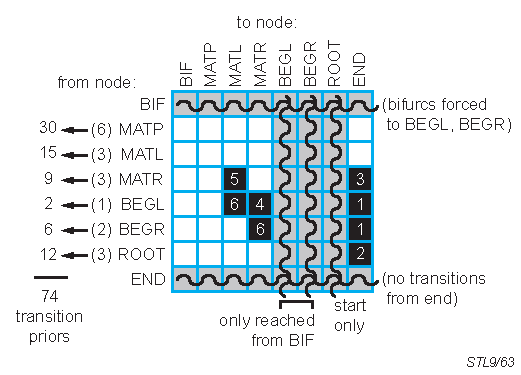
\includegraphics{Figures/stl9-63}
\end{center}
\caption{\small\textbf{Where does the magic number of 74 transition
distribution types come from?} The transition distributions are
indexed in a 2D array, from a unique statetype (20 possible) to a
downstream node (8 possible), so the total conceivable number of
different distributions is $20 \times 8 = 160$. The grid represents
these possibilities by showing the $8 \times 8$ array of all node
types to all node types; each starting node contains 1 or more unique
states (number in parentheses to the left).
Two rows are impossible (gray): bifurcations automatically transit to
determined BEGL, BEGR states with probability 1, and end nodes have no
transitions.  Three columns are impossible (gray): BEGL and BEGR can
only be reached by probability 1 transitions from a bifurcation, and
the ROOT node is special and can only start a model. 
Eight individual cells of the grid are unused (black) because of the
way \prog{cmbuild} (almost) unambiguously constructs a guide tree from
a consensus structure.  These cases are numbered as follows. (1) BEGL
and BEGR never transit to END; this would imply an empty
substructure. A bifurcation is only used if both sides of the split
contain at least one consensus pair (MATP). (2) ROOT never transits to
END; this would imply an alignment with zero consensus
columns. Infernal models assume $\geq 1$ consensus columns. (3) MATR
never transits to END. Infernal always uses MATL for unpaired columns
whenever possible. MATR is only used for internal loops,
multifurcation loops, and 3' bulges, so MATR must always be followed
by a BIF, MATP, or another MATR. (4) BEGL never transits to MATR. The
single stranded region between two bifurcated stems is unambiguously
assigned to MATL nodes on the right side of the split, not to MATR
nodes on the left. (5) MATR never transits to MATL. The only place
where this could arise (given that we already specified that MATL is
used whenever possible) is in an interior loop; there, by unambiguous
convention, MATL nodes precede MATR nodes. (6) BEGL nodes never
transit to MATL, and BEGR nodes never transit to MATR. By convention,
at any bifurcated subsequence $i,j$, $i$ and $j$ are paired but not to
each other. That is, the smallest possible subsequence is bifurcated,
so that any single stranded stretches to the left and right are
assigned to MATL and MATR nodes above the bifurcation, instead of MATL
nodes below the BEGL and MATR nodes below the BEGR.
Thus, the total number 74 comes from multiplying, for each row, the
number of unique states in each starting node by the number of
possible downstream nodes (white), and summing these up, as shown to
the left of the grid.}
\label{fig:magic74}
\end{figure}

\newpage
\section{Acknowledgements}

Infernal relies heavily on HMMER and Easel, originally created by Sean
Eddy. Several others have helped develop these two packages as well,
including Steve Johnson, Alex Coventry, Dawn Brooks, Sergi Castellano,
Michael Farrar, Travis Wheeler, and Elena Rivas.  In particular, the
improved speed of Infernal 1.1 is enabled by research and development
for the HMMER3 project, mainly from Sean, Travis and Michael. Further,
many of the changes made for Infernal 1.1 mirror features in HMMER3,
and were implemented frequently by stealing and slightly modifying
code. Even this guide is based heavily on HMMER3's guide, and some
analogous sections are identical or near identical.  Additionally, the
RSEARCH program \citep{KleinEddy03} from Robbie Klein has also had an
important impact on Infernal, which still includes some of its code.

Sean created and was the lone developer of Infernal up through the
version 0.55 release in 2003. Two graduate students, Diana Kolbe and
Eric Nawrocki, focused on improvements to Infernal for their graduate
work, beginning in 2004. Their efforts combined with Sean's led to
versions 0.56 through 1.0.2. Diana has moved onto a postdoc, but
included a snapshot of the codebase in between the 1.0.2 and 1.1
releases as supplementary material with her thesis. Eric continues to
develop Infernal and is responsible for most of the changes in the 1.1
release.

The concept of HMM banded SCFG alignment implemented in Infernal
derives from Michael Brown's RNACAD software, developed while he was
working with David Haussler at UC Santa Cruz \citep{Brown00}. HMM
filtering for CMs was pioneered by Zasha Weinberg and Larry Ruzzo at
the University of Washington
\citep{WeinbergRuzzo04,WeinbergRuzzo04b,WeinbergRuzzo06}. The CP9 HMMs
in Infernal are a reimplementation of a profile HMM architecture
introduced by Weinberg.

Infernal testing requires \emph{a lot} of compute power, and we are
extremely fortunate to have access to a highly reliable and
state-of-the-art computing cluster, thanks to Jesse Becker, Ron
Patterson and others at NCBI.

Infernal is primarily developed on GNU/Linux and Apple Macintosh
machines, but is tested on a variety of hardware. Over the years,
Compaq, IBM, Intel, Sun Microsystems, Silicon Graphics,
Hewlett-Packard, Paracel, and nVidia have provided generous hardware
support that makes this possible. We owe a large debt to the free
software community for the development tools we use: an incomplete
list includes GNU gcc, gdb, emacs, and autoconf; the amazing valgrind;
the indispensable Subversion; the ineffable perl; LaTeX and TeX;
PolyglotMan; and the UNIX and Linux operating systems.

\label{manualend}


\newpage
\bibliography{master,lab,books,local}
\end{document}
